\documentclass[12pt,oneside,italian]{book}

%\usepackage{breqn}         % automatic equation breaking
\usepackage{microtype}     % microtypography, reduces hyphenation
\usepackage{babel}
\usepackage{amsmath}
\usepackage{hyperref}
\usepackage{graphicx}      % graphics support

% \usepackage{endnotes}
% \let\footnote=\endnote
% 
% \renewcommand{\notesname}{Note}

\usepackage[utf8]{inputenc}

\title{Riassunto di studio \\ per Reti di Calcolatori M}
\author{Daniele Tiles \and Davide Bellettini (revisione)}
\date{2007 - 2014}

\begin{document}
\maketitle
\newpage

\chapter{Introduzione}
L'obiettivo del corso è introdurre modelli e tecnologie per poter superare il 
modello Client/Server (C/S), in modo
da poter:
\begin{itemize}
 \item Migliorare la gestione
 \item Introdurre un supporto alla \textit{qualità del servizio, QoS}: questo è fondamentale, perché solo se un sistema
 presenta QoS, allora si può pensare ad un sistema di retribuzione (Internet, mail e gli altri servizi
lavorano \textit{best-effort}): vi sono sistemi ``più standard'', importanti per i sistemi molto carichi.
\item Sviluppare sistemi in grado di far fronte anche ad alta mobilità, l'integrazione di sistemi legacy.
\end{itemize}
Si tratta quindi di un corso per poter descrivere le tecnologie di sviluppo possibili per poter creare un
\textit{sistema distribuito}: cosa conviene scegliere, quando usare una tecnologia invece che un'altra? Ha senso cercare
di realizzare una nuova tecnologia, un middleware\footnote{Un middleware è un qualcosa che si interpone fra
l'applicazione e i livelli più bassi: fornisce servizi di aiuto per lo sviluppatore, mette a disposizione meccanismi per
poter implementare \textit{diverse politiche}} proprio? Per fare qualche esempio, non ha senso usare CORBA se il sistema
necessita di un unico nodo, dove si deve interagire con componenti Java, oppure si devono usare \textit{agenti mobili}
dove è necessaria la mobilità! Vi è un particolare interesse per il progetto e testing (soprattutto per l'esecuzione e
il deployment).
\chapter{Modelli di computazione}
Per poter sviluppare un sistema distribuito, è utile definire diversi modelli per l'esecuzione, in modo da poter
classificarli (modelli diversi possono avere vantaggi/svantaggi a seconda del sistema che si deve andare a realizzare).
La maggior parte dei modelli purtroppo sono troppo astratti per poter essere realmente utili da un punto di vista
ingegneristico, cioè non riescono a comprendere in toto la \textit{complessità} reale.

Le prime distinzioni che si possono fare sono su come si possono prendere le decisioni:
\begin{itemize}
 \item modelli \textit{statici}: le decisioni vengono prese prima dell'esecuzione. Risulta quindi essere meno
flessibile, e non si può variare nel corso dell'esecuzione, fornendo quindi poca qualità di servizio.
\item modelli \textit{dinamici}: in questo modello le decisioni risultano essere maggiormente costose, proprio perché
si prendono mentre il modello è in esecuzione.
\end{itemize}
Per fare un esempio, il collegamento fra un client e un Name Server come deve essere stabilito? In maniera statica o
dinamica? E fra il client e server? Si tratta di problematiche da risolvere in fase di progettazione, tenendo conto
dei costi. Un middleware introduce questi costi, fornendo possibilità statiche/dinamiche (non esiste un sistema
totalmente dinamico, realmente totalmente aperto).
Una seconda distinzione riguarda la reazione in caso di errori o concorrenza:
\begin{itemize}
 \item modelli \textit{preventivi}: si fornisce un \textit{comportamento garantito}, oppure si previene/evitano
determinati errori. E quindi un sistema rigido, che presenta dei \textit{costi fissi}.
\item modelli \textit{reattivi}: il modello reagisce in maniera dinamica alle situazioni che si presentano: non è
prevista quindi una \textit{politica di default}, non si stabiliscono risorse a priori come nel caso precedente,
fornendo un comportamento più flessibile. I costi risultano essere variabili, a seconda della complessità del sistema
(al crescere degli attori, aumenta il numero necessario di lock/semafori da utilizzare, per esempio). Il costo può
quindi essere limitato a seconda delle esigenze.
\end{itemize}
\textbf{Esempio:} una serie di clienti vogliono accedere in maniera univoca ad
una risorsa unica: si tratta quindi di un problema
di sincronizzazione e mutua esclusione. Si potrebbe risolvere fornendo dei quanti di tempo decisi a priori per ogni
singolo cliente, oppure si fornisce un token, per cui chi lo possiede è l'unico a poter accedere alla risorsa.

È da osservare che un sistema distribuito in generale offre un insieme di \textit{politiche diverse}, che si possono
mescolare a seconda delle esigenze: un sistema moderno infatti deve essere in grado di seguire l'evoluzione dei servizi
per poter sopravvivere (es CORBA: in versioni successive aggiunge supporto al Web).

Un ulteriore modello semplice da descrivere riguarda in che modo le risorse
sono associate alle applicazioni:
\begin{itemize}
 \item Siamo in \textit{monoutenza} se le risorse sono tutte dedicate all'applicazione descritta
 \item Altrimenti si parla di \textit{multiutenza}: più complessa, ma decisamente più diffusa. Infatti, un numero
superiore di applicazioni può portare ad un uso più efficiente delle risorse.
\end{itemize}
A seguito, si può ragionare quindi come sono disponibili le risorse:
\begin{itemize}
 \item Modello \textit{workstation}: le risorse sono concentrate su un unico nodo.
 \item Modello \textit{processor pool}: le risorse sono distribuite, e vengono associate in maniera trasparente al
servizio.
\end{itemize}

\section{Processi o oggetti?}
Un'ulteriore distinzione riguarda su cosa basarsi per descrivere effettivamente come avviene l'esecuzione.
Un primo modello si basa sull'idea del \textit{processo}, che incarna la capacità di esecuzione della macchina. Si
specificano quindi delle operazioni, e si tratta di modelli che tengono conto della macchina su cui si lavora, e
funzionano molto
bene con risorse locali e stato locali. Vi sono più modelli:
\begin{itemize}
 \item \textit{Processi alla Unix}: si tratta di processi pesanti, ognuno dotato
di un proprio stato locale. In questo modello
interessa solo in che modo i processi possono comunicare, essendo lo stato non
condivisibile.
 \item \textit{Processi alla Java}: i processi son leggeri, hanno uno stato
condiviso che può essere usato anche per comunicare.
Risulta essere più facile fare anche dei cambi di contesto, ma si possono
presentare delle interferenze.
\end{itemize}

I thread di una JVM, proprio perché dotati di uno stato condiviso, si possono rapportare con un'altra JVM. I thread
leggeri utilizzano lo stato comune per comunicare.

Un'altra idea riguarda la modellazione basata sul paradigma ad oggetti. È importante ricordarsi che questi son sempre
delle astrazioni, e quindi necessitano di una concretizzazione successiva. Anche qui si possono supporre due diversi
modelli:
\begin{itemize}
 \item \textit{Oggetti passivi}: i classici oggetti alla Java. Rappresentazione l'astrazione di dati su cui delle entità
esterne possono lavorare. Non sono quindi dotati di capacità propria d'esecuzione. Si può quindi avere concorrenza
fra diversi processi che vogliono accedere allo stesso oggetto, non si ha un buon confinamento e si ha scarsa
protezione.
  \item \textit{Oggetti attivi}: sono oggetti dotati di propria
capacitàd'esecuzione. I processi quindi non entrano nell'oggetto, perché vi è
già all'interno dell'oggetto una propria logica di gestione (si ha quindi un
modello a request/response: un processo richiede di poter usare l'oggetto
mediante i ``metodi'' forniti da questo, e questo in base alla sua schedulazione
risponde alla richiesta. È sempre da osservare che un oggetto attivo ha comunque
un proprio stato interno, descritto da una parte sequenziale, ma a cui non vi si
accede con dei metodi, proprio grazie a questa logica interna: i metodi veri e
propri sono utilizzati solo internamente!). Un oggetto attivo è quindi dotato di
una coda delle richieste che si sono presentate, e una sua politica di
scheduling. Si supera in questo modo il problema degli oggetti passivi,
proteggendo del tutto l'oggetto e determinandolo completamente. Un oggetto
attivo quindi, massimizzando la parte sequenziale, si può spostare più
facilmente. Rappresenta lo stesso modello dei servitori paralleli, e, per
esempio, degli agenti mobili. Un oggetto attivo quindi si preoccupa di tutta la
gestione dell'esecuzione internamente (richieste, attività, errori, processi
interni...): si forniscono meccanismi, mediante il quale si possono specificare
delle politiche diverse!
\end{itemize}

Come mai in Java tale modello non è stato implementato? Si tratta di un
\textit{modello molto costoso}, che non presenta delle scorciatoie utili se si
lavorasse solo in ambito locale!
Nei sistemi moderni, in realtà si parla di classi che contengono le definizioni
degli oggetti, e definiscono lo stato interno e i metodi con cui accedere. In
particolare, in generale si parla di semantica per riferimento, che però è in
grado di funzionare solo in un ambito locale. Per riferire in remoto, serve un
supporto esterno. Per esempio, si parla di utilizzare socket, protocolli
standard de facto come TCP/IP...
Tuttavia, è proprio questo il motivo per cui si vengono a definire dei middleware, ovvero delle strutture in grado di
fornire un supporto completo alla comunicazione in remoto. Per esempio, Java Remote Method Invocation è un sistema in
grado di estendere la semantica per riferimento locale, al remoto, cercando di fornire un sistema omogeneo per poter
accedere sia ad oggetti locali che remoti. Nel caso specifico di RMI, per esempio, si utilizza un classico pattern dei
middleware, il \textit{proxy come delegato per la comunicazione}. Si realizzano
infatti uno stub lato cliente e uno skeleton lato
server, che riescono a garantire un qualcosa di simile alla normale comunicazione locale. Si cerca di presentare
un sistema trasparente per l'utente!

Perché quindi non realizzare tutti i riferimenti come riferimenti remoti? È sempre una questione di costo, sarebbe
inaccettabile. Basta pensare a cosa succede ad un oggetto passato via RMI: deve essere serializzabile, e così tutti
i suoi componenti, in maniera che si possa fare marshalling e unmarshalling.
Ciò non è sempre possibile in Java RMI (si pensi ad un oggetto che riferisce un oggetto di tipo File, una risorsa
strettamente locale). Vi sono poi altri problemi da considerare:

\begin{itemize}
 \item Un oggetto remoto viene registrato in un apposito registry, ma se
 viene deattivato? Come viene gestita quindi la persistenza? E lo stato remoto?
 \item Due stub diversi possono riferire lo stesso oggetto remoto? Se sì come si
 gestisce la concorrenza?
 \item Come risolvere i nomi? Si può usare un riferimento fisso, ma l'oggetto
 può essere diverso (ma non è il caso di Java).
 \item Si deve anche passare l'indicatore della classe, perché si possa realmente utilizzare l'oggetto: cosa succede
 se la classe è già presente? Java per esempio controlla mediante l'hash se la classe è effettivamente quella corretta.
\end{itemize}

\section{Deployment dell'applicazione}
Un'applicazione distribuita spesso necessita che sia suddivisa in diversi componenti, anche allocati su nodi diversi!
Un componente è un'entità con una granularità superiore all'oggetto, ovvero introduce comportamento e interazione,
estendendo l'idea dell'oggetto.
Se si hanno quindi diversi componenti, che devono dialogare fra di loro, non è detto che il deployment su una singola
macchina sia la soluzione ideale: infatti, su un solo processore si ha una sequenzializzazione delle operazioni, e
quindi dell'applicazione stessa.
Spesso e volentieri, un middleware non si occupa del deployment, ma deve essere realizzato da chi gestisce l'interazione
fra i componenti. L'allocazione può essere statica, cioè decisa prima dell'esecuzione, oppure dinamica, quindi
durante; quest'ultimo modello permette di poter spostare le risorse a seconda delle esigenze durante l'esecuzione.
Spesso e volentieri, l'allocazione viene realizzata utilizzando dei semplici file batch, rendendola semi-manuale (certe
configurazioni devono poi essere sistemate a seconda dei casi dall'operatore).
L'approccio misto è quello più usato, essendo una via di mezzo fra l'allocazione esplicita (tutta a carico dell'utente)
e quella implicita (decisa in toto dal sistema).

\section{Altri modelli oltre il C/S}
Esistono diversi altri modelli oltre il classico C/S:
\begin{itemize}
 \item \textit{Push}: il servitore fornisce il servizio al cliente
 \item \textit{Pull}: il cliente recupera il servizio che necessita in maniera diretta.
 \item \textit{Modello a delega}: il cliente delega un altro agente per attendere il risultato, e poi lo recupera da
 questo.
 \item \textit{Modello a notifica}: simile al precedente, solo che il delegato notifica al cliente la disponibilità
 del risultato.
 \item \textit{Modello ad eventi}: il tipico modello consumer/provider, in cui chi è interessato si registra a chi
 produce gli eventi.
 \item \textit{Modello a provisioning}: oltre agli end-point, vi sono intermediari interessati al risultato.
\end{itemize}
Di particolare interesse è la classificazione dei modelli a scambio di messaggi:
\begin{itemize}
 \item In fase di progettazione, si parla di sistemi sincroni se si è interessati al risultati, altrimenti asincroni.
 \item In fase implementativa, si parla di comunicazione bloccante se il richiedente si blocca in attesa del risultato,
 altrimenti non bloccante
\end{itemize}
Oltre alla classicazioni principali, altre caratteristiche con cui si possono classificare i modelli a scambio di
messaggi:
\begin{itemize}
 \item In fase di progettazione si parla di:
 \begin{itemize}
  \item un \textit{sistema simmetrico} se mittente e ricevente si conoscono
  (rarissimo) oppure \textit{asimmetrico} (caso tipico :C/S).
  \item un sistema diretto (cioè se avviene una comunicazione diretta fra i
  processi), oppure indiretto (se si utilizzano strutture tipo le socket)
 \end{itemize}
 \item In fase di implemtazione si parla di:
 \begin{itemize}
  \item un \textit{sistema bufferizzato} se la comunicazione richiede un certo
  numero di messaggi prima di poter trasmettere
  \item \textit{sistemi reliable} se possono fornire QoS, senza perdere
  messaggi.
 \end{itemize}
\end{itemize}
Nel caso si introduca un terzo oggetto che faccia da mediatore, si può quindi lavorare in maniera sincrona ma non
bloccante: è il mediatore che resta in attesa, sganciando il ricevente. Si possono avere due diverse modalità:
\begin{enumerate}
 \item \textit{Oggetti poll}: è un contenitore per la risposta alla richiesta, che viene periodicamente interrogato
 dal ricevente con un sistema a polling. Si ha così una comunicazione a 3 entità. In questo modello, il ricevente
 deve sapere dove si trova l'oggetto poll, e vi deve essere un oggetto per ogni risultato. E conveniente se si hanno
 operazioni corte, e attese brevi.
 \item \textit{Oggetti callback}: è sempre un oggetto che conterrà il risultato, ma dotato di una sua vita
 indipendente, e dotato di codice particolare da eseguire quando giunge il risultato. E lui quindi a dover fornire il
 risultato al richiedente, svincolandolo del tutto da questo! Conveniente in caso di operazioni lunghe, indipendenti
 dal chiamante.
\end{enumerate}
Spesso e volentieri, questi intermediari vengono realizzati da proxy, che sono in grado di ridurre la complessità
logica della soluzione, integrando diverse funzionalità.
In un modello basato sugli eventi, si ha un fortissimo disaccoppiamento (non vuol dire che non si conoscono, ma che
non è necessario che siano attivi contemporaneamente per poter fare la comunicazione; è una caratteristica
fondamentale per i middleware) fra le entità interessate al risultato, e quelle che forniscono i servizi. In questo
modello si ha quindi un'interazione molti a molti, per cui si può facilmente mappare il multicast. In generale gli
eventi non sono persistenti, tuttavia non è l'unico modello possibile.
\section{Spazi di tuple}
Un modello che deriva dall'astrazione della memoria condivisa e della comunicazione, e che garantisce il
disaccoppiamento fra le varie entità è lo spazio di tuple. È un meccanismo generale per la comunicazione e la
sincronizzazione, in cui si specifica uno spazio di informazioni fortemente tipato. (Una tipica informazione può essere
\texttt{<mittente, destinatario, data>}, per cui tutti i dati devono essere
diversi perché possa essere inserita).
Si hanno quindi due operazioni principali: la \textit{out} consiste nell'inserire nello spazio delle tuple un nuovo
messaggio, mentre la \textit{in} (bloccante) estrae la prima tupla che fa match
con il criterio indicato (in caso di più tuple che facciano match, è una scelta
non deterministica). Ovviamente, si avrà sempre un numero inferiore di in
rispetto alle out. Se la in è \textit{completamente specificata}
\footnote{specifichiamo l'esatto contenuto della tupla che stiamo cercando}, si
parla di sincronizzazione e non di comunicazione. Uno spazio di tuple permette
anche l'introduzione di QoS, grazie alla persistenza della tupla nello spazio.
Gerlenter, con Linda, presenta due diversi modelli:
\begin{itemize}
 \item \textit{A ring}: si partiziona lo spazio delle tuple, per cui ogni nodo conosce precedente e successivo: si ha
 una conoscenza locale, quindi limitata. Un produttore può fare una out su un qualsiasi nodo, e il messaggio fa un
 ciclo per verificare che non sia già presente su un qualche nodo. Lo stesso discorso vale per la in, che fa un giro
 fino a trovare un messaggio che fa match. In Linda sono state considerate ovviamente delle problematiche di
 replicazione (il messaggio deve essere ripetuto? Ma quindi lo si deve togliere da tutti i nodi che lo contengono),
 sfruttando gli hash dei messaggi
 \item \textit{A matrice}: le out vengono eseguite sulle righe, mentre le in si fanno sulle colonne.
\end{itemize}
\section{Modelli a contenimento}
Si tratta di supporti presenti in ogni middleware: sono funzionalità che aggregano diverse attività utili, che si
possono replicare. In questo modo, uno sviluppatore si concentra soltanto sullo sviluppo della business logic vera e
propria, utilizzando le politiche di default fornite dal middleware per quanto riguarda il supporto al tempo di vita,
il gestore della concorrenza, fornire la QoS, sistemi di nomi... Fondamentalmente, un container è un delegato che si
comporta come supervisore di certe attività.
\section{Il problema della trasparenza}
Esistono diversi signicati per la trasparenza: per esempio, si intende per l'allocazione l'indipendenza dalla località
delle risorse. In generale, per trasparenza si intende un sistema in grado di fornire all'utente finale un comportamento
omogeneo, anche se ai livelli sottostanti sta lavorando con oggetti/servizi diversi (remoti/locali, server
principale/copia...).
Non è sempre un elemento positivo, perché in molti casi i sistemi son così complessi, che non si possono gestire in
maniera totalmente trasparente: si richiede l'intervento dell'utente. Un esempio è nella trasparenza dell'allocazione:
se non sappiamo dove si trova l'utente, come facciamo a dargli il servizio desiderato? La trasparenza non è corretta
a livello di infrastruttura in questo caso; l'utente infatti è sempre più coinvolto.
Per esempio, TINA-C\footnote{Si tratta di un consorzio di aziende per le telecomunicazioni, con l'obiettivo di andare
oltre OSI: l'idea è quella di immaginare anche i possibili servizi, fornendo un modello più coordinato, e
un'infrastruttura con molti provider: si definisce un accordo/negoziazione fra i fornitori dei servizi e i clienti,
per poter per esempio stabilire la QoS, e quindi si fornisce il servizio con i parametri indicati} prevede sia un
sistema trasparente, che un sistema non trasparente in cui si possano definire le risorse inizialmente, e quindi
introdurre la trasparenza.
\section{Le macchine astratte}
Sono stati sviluppati diversi modelli per l'esecuzione, ma alla base vi è la
\textit{Random Access Machine}: è una macchina special purpose, con codice
inalterabile, in grado di eseguire istruzioni in sequenza (tutte le istruzioni
hanno la stessa durata), memoria composta da una sequenza di parole capaci di
contenere un intero e un sistema di input e uno di output.
Un primo modello per la comunicazione è la \textit{Parallel RAM} (PRAM), in cui
si immagina diversi programmi da eseguire contemporaneamente. Una PRAM è
costituita quindi da P macchine RAM, ognuna delle quali esegue un programma, e
ad ogni clock vengono eseguite P istruzioni. Alla base vi è una memoria
condivisa, per tutte le macchine, dove scrivere e leggere i risultati (anche i
dispositivi di I/O sono unici per tutte le macchine). Si tratta di un modello
MIMD (Multiple Instruction Multiple Data) sincrono, per cui quando tutti i
programmi finiscono, anche la macchina termina. Essendo dotata di un'unica
memoria, come devono essere strutturate le operazioni? La concorrenza è un
requisito difficile da realizzare, in confronto al mettere le operazioni in
sequenza. Le diverse PRAM si possono quindi categorizzare a seconda della
tipologia delle operazioni (in generale si hanno letture concorrenti e scritture
sequenziali (CREW - Concurrent Read Exclusive Write); la concorrenza è invece
utilizzata per il sistema di I/O, per limitarne il collo di bottiglia). Un PRAM
è difficile da realizzare perché non è scalabile.
Un secondo modello è il \textit{Message Passing RAM}, che è sempre una
collezione di RAM, ma ognuna con la sua memoria dedicata (i sistemi di I/O son
sempre condivisi). Si ha quindi che le diverse macchine comunicano mediante dei
canali prestabiliti (vi devono essere almeno P-1 connessioni). Si hanno
istruzioni ad hoc, cioè delle send e receive con rendez-vous, una semantica
sincrona: questo vuol dire che un'operazione sblocca la sua duale. Una MP-RAM è
più facilmente realizzabile, e rappresenta meglio un modello locale. Se per
esempio si volesse eseguire un broadcast,
servirebbero almeno P-1 istruzioni, mentre una PRAM, per quanto più difficile
da realizzare, richiederebbe una sola operazione: è un modello con maggiore
capacità espressiva. Restano comunque entrambi dei modelli troppo astratti per
poter essere implementati realmente. Aggiungendo vincoli e limitandoci quindi ad un'ipotesi di località, il progetto
risulta più facilmente realizzabile.
\section{Indicatori dell'efficienza}
In generale, ci si limita alla complessità temporale, $T_P(N)$, dove $P$ è il numero di processori considerati: se è
pari ad 1, siamo in un ambiente sequenziale.
Un primo indicatore è lo speed-up, che indica l'incremento di prestazioni se si introducessero P processori:
\begin{equation}
S_P(N) = \frac{T_1(N)}{T_P(N)} > 1
\end{equation}
Tuttavia, bisogna sempre tener presente che non tutti i programmi si possono
parallelizzare: ciò dipende se vi sono troppe dipendenze fra le sotto parti.
Un altro indicatore è l'efficienza nell'uso delle risorse:
\begin{equation}
 E_P(N) = \frac{S_P(N)}{P}
\end{equation}
Ma quindi, ciò corrisponde a dire:
\begin{equation}
 E_P(N) = \frac{T_1(N)}{T_P(N)} \cdot \frac{1}{P}
\end{equation}
Possiamo quindi definire lo speed-up massimo:
\begin{equation}
 max(S_P(N)) = P
\end{equation}
E l'efficienza massima:
\begin{equation}
 max(E_P(N)) = 1
\end{equation}
Sotto queste condizioni si avrebbe che tutti i processori lavorano al massimo, ovvero non abbiamo processori idle che
possono risultare inutili. Questi sono coefficienti statistici, validi per tutto l'algoritmo. Quello che si può
osservare è che la situazione ideale la si avrebbe se lo speed-up dipendesse in maniera lineare dal numero dei
processori. Una soluzione ideale non interessante sarebbe se si distribuisse i compiti ai processi in maniera uguale (un
programma totalmente parallelo!), raccogliendo solo alla fine il risultato. In realtà, i casi più interessanti sono
quelli dove si presentano delle dipendenze, per cui necessariamente vi deve essere una parte sequenziale: questo caso
presenta quindi una comunicazione intrinseca, indipendente dal deployment che si viene a realizzare.
Si possono quindi studiare diversi casi basandosi sui fattori di interesse $N$ e $P$. In particolare, si può definire
come fattore di carico, o loading factor:
\begin{equation}
 L = \frac{N}{P}
\end{equation}
che definisce la complessità come viene suddivisa su ogni nodo. Vi possono essere diversi casi:
\begin{itemize}
 \item \textit{N uguale a P}: su ogni processore viene posta una parte molto semplice del problema. Si dice ipotesi
 di identità.
 \item Dipendenza di N da P
 \item Indipendenza, interessante al crescere di N
\end{itemize}
La legge di Grosh stabilisce che la soluzione migliore risulta essere quella
di lavorare sempre nel concentrato... ma ciò non è sempre possibile! Se per
esempio vi sono risorse limitate? Oppure, oltre un certo valore di N, non si
riesce più a lavorare nel concentrato, e la legge è sicuramente inutile nel caso
di vincoli, tipo la presenza di risorse distribuite.
\begin{figure}[htbp]
 \centering
 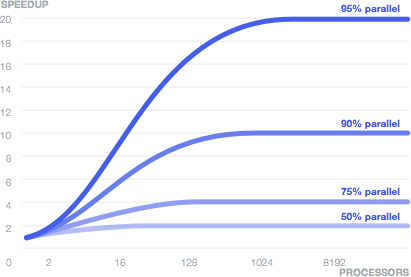
\includegraphics[width=0.8\textwidth]{Images/amdahl.png}
 \caption{Legge di Amdahl [reactivemanifesto.org]}
 \label{fig:amdahl}
\end{figure}
La legge di Amdhal (figura \ref{fig:amdahl}) stabilisce che vi è un limite alla
possibile parallelizzazione, dato che ogni programma è
costituito da una parte parallela e una parte sequenziale, e quest'ultima limita lo speed-up: si ha quindi che non
cresce linearmente, ma tende a un valore asintotico! Nella situazione migliore immaginabile, con le risorse
correttamente allocate, si ha quindi che si avrà uno speedup fisso, mentre sarà l'efficienza a variare a seconda
dell'architettura del sistema!
Come calcolare quindi lo speed-up massimo? Si vuole avere il numero di processori tali che si abbia la minore
complessità del problema, realizzando un sistema fortemente caricato: si definite quindi l'heavily loaded limit:
\begin{equation}
 T_{HL} = \liminf_P{T_P(N)}
\end{equation}
Infatti, si lavora bene caricando molto ogni processore, i quali quindi lavorano per tutto il tempo necessario:
abbiamo quindi in questo modo un buon uso delle risorse.
Tuttavia, per la legge di Amdhal, dobbiamo ricordare che vi è anche una parte sequenziale in ogni programma... che è
proprio la parte di comunicazione fra i diversi processori! Al crescere del numero dei processori, si ha quindi
che lo speed-up diminuisce, allontanandosi dal valore massimo; questo degrado delle prestazioni è dovuto proprio al
peso crescente della comunicazione fra i processori, che diventa fondamentale\footnote{per esempio se la parte
sequenziale è $\frac{1}{5}$ del totale lo speedup massimo sarà il reciproco, ovvero 5}.
\section{Caso di studio: somma di N numeri}
Una possibile soluzione, imponendo la condizione d'identità, è quella di utilizzare un albero binario per fare la
sommma: le radici sommano i numeri, che passano il risultato al padre, e così via. Supponendo quindi un albero con
profondità H, possiamo osservare che $N = 2{H+1}$ e $P = 2^{H+1} - 1$, per cui P è simile a N . Si ha che quindi:
\begin{align}
T_P(N) &= O \left(H \right)              \nonumber \\
       &= O \left(\log_2(N)\right)      \nonumber \\
       &= 2 \cdot \log_2 \left(N\right)
\end{align}
Perché 2? Perché abbiamo 2 comunicazioni in ogni nodo. Possiamo quindi valutare l'efficienza di questa architettura:
\begin{equation}
 E_P \left( N \right) = O \left( \frac{1}{log_2\left(N\right)} \right)
\end{equation}
Ma quindi, al crescere di N, l'efficienza tende a 0! Per quanto riguarda lo speedup, si ha che non lavorano tutti i
nodi, ovvero più si risale l'albero e meno i processori lavorano (il processore radice deve attendere, ovvero tempo
di idle, che tutti gli altri abbiano finito!). Se invece avessimo un flusso di dati, i processori risulterebbero
tutti sempre impegnati (potremmo risolvere un insieme di problemi).
Come si possono quindi mantenere sempre impegnati i processori? Si deve incrementare il lavoro sul singolo processore,
per cui:
\begin{equation}
 L = \frac{N}{P} \gg 1
\end{equation}
e quindi la complessità deve essere superiore al numero dei processori: su ogni nodo si ha quindi un certo numero di
valori da sommare. Ciò si può ottenere per esempio con un albero fisso, ovvero un numero di processori fissi. Infatti:
\begin{equation}
 T_P\left(N\right) = O \left(L + \log_2 \left(P\right)\right)
\end{equation}
I due componenti rappresentano rispettivamente il tempo di computazione e quello di comunicazione.
\begin{align}
 S_P(N) &= \frac{T_1(N)}{T_P(N)} \nonumber \\
        &= O \left( \frac{N}{\frac{N}{P} + \log_2(P)} \right) \nonumber \\
        &= O \left( \frac{P}{1} + \frac{P}{N \cdot \log_2(P)} \right)
\end{align}
Per cui, lo speed-up tende effettivamente a P
\begin{align}
 E_P(N) &= \frac{S_P(N)}{P} \nonumber \\
        &= O \left(\frac{1}{1} + \frac{1}{N \cdot \log_2(P)}\right)
\end{align}
E l'efficienza tende ad 1. Quindi, caricando al massimo i processori ed usandoli correttamente, si ottiene speed-up
ed efficienza massimi.
\section{Considerare l'I/O}
In questi indicatori si è tuttavia lasciato da parte il problema dell'I/O, che spesso è il vero collo di bottiglia in
diverse architetture. Inoltre, vi son diversi fattori che possono influenzare l'efficienza e lo speed-up
dell'architettura, come il deployment reale. Si possono quindi estendere gli indicatori considerando l'effetto
generale dell'\textit{overhead}, $T_0(N)$, che rappresenta le risorse e il tempo
realmente utilizzato per la comunicazione
(caso ideale di deployment):
\begin{equation}
T_0(N) = \left|T_1(N) - P \cdot T_P(N)\right|
\end{equation}
Ma quindi, si ha che:
\begin{equation}
 T_P(N) = \frac{T_0(N) + T_1(N)}{P}
\end{equation}
E si ha che che lo speed-up risulta essere:
\begin{equation}
 S_P(N) = \frac{P \cdot T_1(N)}{T_0(N) + T_1(N)}
\end{equation}
E che l'efficienza risulta essere:
\begin{equation}
E_P(N) = \frac{1}{1 + \frac{T_0(N)}{T_1(N)}}
\end{equation}
Per cui l'efficienza non sembra dipendere dal numero dei processori... in realtà,
è proprio $T_0(N)$ a dipendere dal numero dei processori: l'overhead dipende dal numero di processori impegnati.
Supponiamo quindi di avere come obiettivo per l'architettura di mantenere costante l'efficienza:
\begin{align}
                            E_P(N) &= \frac{1}{1 + \frac{T_0(N)}{T_1(N)}} \nonumber \\
 E + E \cdot \frac{T_0(N)}{T_1(N)} &= 1                                   \nonumber \\
             \frac{T_0(N)}{T_1(N)} &= \frac{1 - E}{E}                     \nonumber \\
                            T_0(N) &= \frac{1 - E}{E} \cdot T_1(N)        \nonumber \\
                            T_0(N) &= K \cdot T_1(N)
\end{align}
Se K fosse veramente una costante, saremmo in isoefficienza. Un sistema isoefficiente indica che, se manteniamo
costante la complessità e aumentiamo il numero dei processori, l'efficienza non varia. Il valore di K quindi determina
se il sistema ha un buon comportamento. In particolare:
\begin{itemize}
 \item \textit{K piccolo}: il sistema è altamente scalabile. Al crescere di K quindi la scalabilità del sistema decresce
 \item Se non è costante ma funzione dei processori, allora il sistema non è scalabile.
\end{itemize}
I sistemi reali sono scarsamente scalabili.
\section{Conclusioni}
Un progetto deve essere valutato attentamente, per cercare di dimensionarlo in maniera corretta: nel caso di una
macchina singola l'heavily loaded limit è un ragionamento corretto, ma bisogna ricordarsi che si deve sempre cercare di
parallelizzare (non utilizzare la legge di Grosh). Per esempio, qual è il numero ideale di processi da realizzare? Si
può ben pensare che avere meno processi di processori risulti in processori che non lavorano, e quindi in un sistema
non efficiente: il limite superiore quindi è che il numero dei processi sia lo stesso del numero dei processori. Un
processore è idle quando comunica, quindi si dovrebbe limitare la comunicazione, e quindi troppi processi comunicano
troppo.
In realtà, statisticamente si ha che un processore che lavora con 20 processi presenta ancora lo stato di idle: un
centinaio di processi per processore è un numero adeguato.

\chapter{Modelli per la replicazione}
Un obiettivo per poter fornire della qualità di servizio è ovviamente quello di
poter offrire un servizio continuativo,
stabile: se il servizio non viene erogato, non si è remunerati (anzi, in
determinati ambiti si ha proprio un danno economico perché si possono
presentare anche delle richieste di risarcimento; in certi ambiti si parla anche
di rischi umani).
L'obiettivo è quindi quello di realizzare un sistema \textit{fault tolerant},
resistente ai guasti. Sono invarianti che devono essere comunque garantiti.
\section{Definire i comportamenti errati del sistema: cause ed effetti}
I possibili guasti si possono catalogare in maniera logica:
\begin{itemize}
 \item Si parla di \textit{failure} quando il sistema presenta un comportamento
diverso dagli invarianti di sistema
previsti: ciò è dovuto a un sistema progettato male. Il failure è l'effetto
visibile, riscontrabile dall'utente.
 \item Un \textit{errore} è invece il difetto che genera un failure del sistema,
 la causa concreta che ha portato il sistema in uno stato non corretto.
 \item Un \textit{fault} infine è proprio il comportamento che si è venuto a
verificare che ha portato il sistema a generare un
 failure: corrisponde quindi proprio alla causa a monte.
\end{itemize}
I fault si possono classificare a seconda di quanto si ripetono:
\begin{itemize}
 \item Sono \textit{permanenti} se si ripresenta in maniera periodica: sono
quindi facili da individuare, e facili da
 risolvere. Si parla di Bohrbug per errori che si ripetono facilmente,
riproducibili, che si possono quindi osservare
 e correggere facilmente.
 \item Se invece sono \textit{transienti}, sono più dicili da notare. Si parla
di errori di tipo Eisenbug, e sono molto
 dicili da eliminare.
\end{itemize}

\section{Ipotizzare il guasto}
Esistono diversi parametri per poter giudicare la disponibilità di un
servizio/sistema.
Un sistema è fault tolerant se garantisce la \textit{dependability}, ovvero si
ha confidenza per qualunque aspetto
progettuale. Ciò comporta che il sistema debba garantire:
\begin{itemize}
 \item \textit{Reliability}: deve essere affidabile, in ogni modo il sistema si
comporta correttamente rispetto agli
invarianti che sono stati imposti. È quindi un sistema corretto.
 \item \textit{Availability}: indica la disponibilità nel tempo del sistema. La
risposta da parte del sistema deve
arrivare entro una certa deadline prestabilita.
\end{itemize}
Per poter garantire la disponibilità del sistema a fronte di guasti, si devono
fare delle ipotesi sul guasto. In
generale, la procedura di ripristino consiste infatti prima
nell'identificazione del tipo di guasto, e in base a ciò si
cerca di riattivare con la corretta procedura il servizio (fase di recovery).
In generale, si utilizza l'ipotesi del \textit{fault singolo}, ovvero nel
sistema si può presentare un singolo guasto:
solo quando il sistema torna operativo, si ha che si potrebbe presentare un
ulteriore fault. Quest'ipotesi è necessaria
per poter semplicare il trattamento del recovery. Per poter definire ciò, è
necessario conoscere:
\begin{itemize}
 \item \textit{Il Time To Repair}, TTR, che è il tempo necessario per
accorgersi e per poter correggere il guasto
 \item \textit{Il Time Between Failure}, ovvero il tempo che intercorre fra due
failure (oppure la media, MTBF).
\end{itemize}

L'obiettivo è quindi che il TTR sia inferiore in maniera stretta al (M)TBF.
Mediante l'ipotesi del guasto singolo, si può osservare che se abbiamo più
copie in grado di fornire il servizio, si
può specificare il numero di fault tollerabili e identificabili. Se avessimo
solo due copie, non possiamo tollerare un
guasto, ma possiamo identificarne uno. Con già 3 copie, un guasto si può
tollerare,
perché comunque restano due macchine con cui identificare i guasti successivi:
si riescono così ad identificare 2 guasti. La generalizzazione è che se si
hanno $3t$ copie, si tollerano massimo $t$ guasti.\footnote{Non si fanno ipotesi
sul tipo di guasto, ma solo sul fatto che è singolo} Si possono quindi
ridefinire le proprietà precedenti in base a questi valori:
\begin{itemize}
 \item La \textit{reliability} è il valor medio sulla
 disponibilità/indisponibilità della risorsa considerata
 \item L'\textit{availability} si può esprimere come la percentuale utile di
lavoro che il sistema riesce ad offrire:
 \begin{equation}
  A = \frac{MTBF}{MTBF + MTTR}
 \end{equation}
\end{itemize}
In particolare, si possono distinguere i casi di lettura e scrittura: infatti,la
lettura non modifica lo stato, per cui si può fornire un servizio di lettura
anche se vi sono diverse copie non funzionanti. Viceversa, per garantire uno
stato coeso fra tutte le copie, la scrittura richiede che tutte siano
disponibili.
La reliability si può anche vedere come la probabilità che un servizio sia
disponibile per un certo intervallo di tempo (a 0 deve corrispondere con
l'availability).
Esistono altre proprietà fondamentali, come la correttezza e la vitalità: la
prima definisce che comunque sia, il risultato fornito dal sistema sarà
corretto, la seconda invece stabilisce che comunque si raggiungerà l'obiettivo.
L'ideale sarebbe disporre di entrambe le proprietà, così da poter mascherare i
fault: si può ottenere mediante oppurtune tecniche di replicazione spaziali e/o
temporali:
\begin{itemize}
 \item Se si hanno diverse macchine, che eseguono ognuna un algoritmo diverso ma
 forniscono lo stesso risultato, garantiamo la massima correttezza
 \item Se si hanno invece diverse macchine ognuna con un compito specifico, si
 ottimizza lo throughput del sistema
\end{itemize}
Una singola macchina non basta per \textit{identificare e correggere} un guasto!
La replicazione è fondamentale, almeno per fare monitoring (utilizzo di cluster
per fare il controllo di una risorsa): si potrebbero utilizzare delle specifiche
parti per controllare e correggere l'architettura, ma è necessario rispettare
sempre il principio della minima intrusione: il rischio sarebbe che troppe
risorse sono allocate solo per verificare che il sistema funzioni correttamente,
riducendone l'efficienza! La replicazione è un costo che si va ad aggiungere al
sistema: ma in generale si tratta di un costo fisso, a fronte di possibili costi
molto peggiori in caso di fallimento del sistema!
\section{Possibili guasti}
I guasti si possono anche classificare in base alla loro riconoscibilità da un
sistema (processore esterno):
\begin{itemize}
 \item \textit{Fail-stop}: un processore si ferma perché non rispetta un
 invariante, e questo viene identificato dagli  altri processori
 \item \textit{Fail-safe}: come il precedente, tranne che gli altri processori
 non se ne accorgono: in questo caso quindi non è identificato, ma potrebbe
essere tollerato (dipende dall'architettura stessa).
 \item \textit{Fallimento di tipo bizantino}: il processore termina presentando
però comportamenti assolutamente casuali.
\end{itemize}
Nelle reti di calcolatori si possono poi presentare ulteriori generi di guasti,
dovuti alla mancata totale ricezione/trasmissione di messaggi
(\textit{send/receive omissions}), oppure anche al fatto che un processore si
blocca. Le reti poi possono aggiungere problemi (se un router per esempio non
risponde più, si potrebbe avere che la
rete risulta partizionata in due sottoreti, incapaci di comunicare fra di loro).
\section{Architetture per garantire la fault-tolerance}
Nel corso del tempo sono state pensate e realizzate diverse tipologie di
architetture in grado di fornire questo genere
di servizio.

Una prima ipotesi operativa è quella di realizzare un sistema con vera e
propria replicazione hardware, per cui si
hanno due possibilità:
\begin{enumerate}
 \item o si realizza un'architettura in cui vi è \textit{una sola macchina a
 lavorare, mentre un'altra ne controlla il corretto  funzionamento}, per cui
 interviene solo in caso di guasto. Per esempio, per avere la correttezza si
 potrebbe  avere che a una determinata richiesta rispondano tutte le macchine,
 ma la risposta viene controllata prima di essere fornita.
 \item oppure si realizza un \textit{sistema con cluster}, dove si aggiunge una
 logica di controllo che è in grado di stabilire se una risorsa è disponibile o
 meno, e  quindi è in grado di escluderla dal sistema. Al crescere delle risorse
 aumenta la probabilità di guasti, quindi si devono utilizzare algoritmi
 efficienti per identificarli correttamente: si vuole un \textit{metalivello
 efficiente}!
\end{enumerate}

Un'ipotesi spesso comune è quella della memoria stabile\footnote{Si potrebbe
realizzare mediante la tecnologia RAID,
Redundant Array of Inexpensive Disks; è un sistema a basso costo, inizialmente
realizzato per poter velocizzare la
lettura e quindi per poter fornire un semplice supporto alla replicazione. Le
operazioni sui dischi son quindi
coordinate. In realtà, quando un disco si guastava, essendoci problemi nel
sistema di gestione non si aveva mai una
replicazione veramente buona}: si vuole realizzare un sistema per cui la
memoria persistente dell'architettura non
fallisca mai (sempre disponibile, sempre corretta). Una possibilità per
realizzare ciò consiste nell'utilizzare due
dischi, e fare in modo che ogni blocco sia replicato in maniera uguale su
entrambi, con probabilità d'errore congiunta
nulla (caso dell'errore singolo). Si ha che quindi i singoli blocchi possono
indicare la presenza di errori o meno
(omissions), con l'uso di appositi codici di controllo. Mediante questi
indicatori infatti si ha il controllo se le
copie sono uguali o meno:
\begin{enumerate}
 \item Sulla seconda copia potrei avere dei valori non corretti
 \item Sulla seconda copia potrei avere dei valori corretti ma diversi dalla
prima copia
\end{enumerate}
Il secondo caso in realtà è il peggiore, dovuto magari a problemi di
aggiornamento sulla seconda
copia\footnote{Osservazione: è sicuramente conveniente un'indicazione di tempo
per la scrittura, in maniera tale da
poter aggiornare tutte le copie al dato più recente effettivamente presente}:
clienti che accedono alla seconda copia
prima della fase di recovery non potrebbero accorgersi che il dato è stale.
Ogni operazione deve procedere su tutte le
copie quindi per poter garantire risultati corretti! Tale sistema è sicuramente
costoso e difficile da realizzare.
Un ulteriore aspetto riguarda un sistema software per fare il monitoraggio
delle risorse, necessario e conveniente da mettere in parallelo al sistema di
recovery hardware: si tratta quindi di progettare degli appositi protocolli e
sistemi in grado di permettere all'applicazione di ripartire con il minimo costo
e nel minimo tempo. Il problema di ciò è che un sistema software del genere
sfrutta le stesse risorse dell'applicazione (CPU, RAM...), riducendone
l'efficienza: si deve quindi progettare il tutto rispettando il
\textit{principio della minima intrusione}, limitando il più possibile quindi le
risorse allocate al metalivello di monitoring/supporto dell'applicazione. La
replicazione presenta dei costi elevati in termine di realizzazione, ma anche di
progettazione ed uso delle risorse, quindi deve essere attentamente studiata.
Ipotizzare guasti singoli semplifica la realizzazione dei protocolli, per
esempio.

Una possibile realizzazione è un sistema tandem, cioè in cui tutto è
raddoppiato: l'idea è quella di realizzare un
sistema fail-safe, per cui una CPU identifica l'errore. Ovviamente, un sistema
del genere è complesso e costoso.
\section{Copie calde e copie fredde}
Vi sono due possibili modelli per la replicazione, e dipendono dal
comportamento delle copie:
\begin{itemize}
 \item \textit{Copie fredde}: vi è un'unica copia attiva che funziona, più
diverse copie dormienti. Deve essere quindi
 presente anche un manager del sistema, in grado di attivare in caso di
necessità una delle copie dormienti (ovvero se
 la copia principale presenta un fault e smette di lavorare correttamente). Il
manager si preoccupa quindi di attivare
 una nuova istanza dell'oggetto solo quando la precedente non funziona. Questo
sistema presenta un alto tempo di
 configurazione, e ha il problema che lo stato non è direttamente salvato sugli
oggetti in standby (si dovrebbe
 recuperare in un qualche altro modo...).
 \item \textit{Copie calde}: in questo caso vi sono diversi oggetti, pronti a
sostituire una copia che non funziona:
 l'idea è che in questo caso vi sia invece un protocollo di ruolo, in grado di
indicare ad ogni copia che comportamento
 deve assumere (è la principale o meno): infatti, la copia principale è attiva,
ovvero in grado di salvare lo stato,
 mentre le altre son passive, che vengono sempre aggiornate ad ogni modifica
sulla copia attiva. Se fallissero anche
 tutte le copie calde, si può ripiegare su un sistema a copie fredde, in grado
di inizializzare una nuova copia.
\end{itemize}
\section{Gestione delle risorse}
La replicazione delle risorse è necessaria per un sistema distribuito, perché
introducendola si può garantire la
fruizione del servizio. In un progetto quindi si deve considerare come allocare
le risorse sui vari nodi, e con che
grado di replicazione: risorse replicate significa quindi che si hanno copie
multiple delle risorse su nodi diversi!
Maggiore è l'importanza della risorsa, maggiore deve essere il suo grado di
replicazione.
Si possono ipotizzare sempre due modelli base:
\begin{itemize}
 \item \textit{Modello passivo}: una sola risorsa lavora, e le altre sono in
attesa pronte a sostituirla in caso di
 failure. Il modello generale è quindi quello di un master con una serie di
slave, organizzati in maniera gerarchica.
 Se il numero di partecipanti è limitato non è costoso, ed è il modello più
facile da implementare (ha un protocollo
 chiaro e semplice). Il grado di replicazione è quindi indicato dal numero di
copie passive disponibili.
 \item \textit{Modello attivo}: tutte le copie eseguono assieme per ottenere il
risultato desiderato. Sono quindi tutte
 attive, ed è necessario predisporre una parte di controllo abbastanza
complessa, quindi la modellazione e
 l'implementazione sono più costose (tutte le copie devono avere l'input, e
tutti gli output devono essere confrontati).
\end{itemize}
In entrambi i modelli non si lavora in maniera sequenziale, ma parallela: le
copie possono comunque svolgere anche
altri compiti, eseguire più operazioni contemporaneamente!

Nel primo modello si deve pensare ad un sistema per tenere aggiornate le copie
fredde: si utilizzano quindi dei
checkpoint, per cui lo stato viene trasferito e replicato sulle copie fredde...
ma quando farlo?
\begin{itemize}
 \item Se lo si fa prima di fornire la risposta al cliente, si garantisce
un'alta efficienza a scapito della
 correttezza (se gli slave presentano un guasto, non saranno aggiornati
correttamente)
 \item Se invece si attende che tutte le copie garantiscano di aver ricevuto
l'aggiornamento prima di spedire la
 risposta, il sistema è corretto, ma la risposta avrà un tempo molto lungo.
\end{itemize}
L'aggiornamento può essere eseguito periodicamente (\textit{time-driven})
oppure ad ogni volta che si presenta un nuovo
evento (\textit{event driven}). Quest'ultima politica risulta essere
maggiormente dinamica e complessa da realizzare.
Per esempio, un evento potrebbe essere scatenato dall'inizio del servizio della
richiesta (estrazione dalla coda delle
richieste), e terminare alla fine per poter fare il checkpoint.

Le operazioni poi possono correlate o meno, e quindi anche il checkpoint
potrebbe essere correlato! In questo caso,
servono delle informazioni dall'utente su quando conviene fare il checkpoint
(tipicamente, si attende che si giunga ad
uno stato stabile e poi lo si esegue).

Serve quindi la trasparenza? Il cliente deve sapere chi contattare se il master
non è raggiungibile, quindi no! Deve
avere idea che non sta interagendo con la copia principale, per poter sfruttare
le risorse per potersi collegare alla
risorsa secondaria mediante un opportuno sistema di nomi. Inoltre, a seconda
della complessità del master, potrebbe
essere conveniente farlo ritornare direttamente come master, invece che come
slave. Si può comunque realizzare così una
sorta di \textit{fault-transparency}, per cui dall'esterno la risorsa sembra
reggere diversi fault e riesce a fornire
un servizio con continuità.

Infatti, sarebbe meglio che all'esterno non si sapesse il grado di replicazione
di una risorsa, perché altrimenti
sarebbe una decisione distribuita mediante il deployment: è in realtà il
middleware ad accorgersi e a fare da supporto,
contattando la nuova copia: per il client è tutto trasparente!

Nel caso di copie attive, il client come le deve conoscere? Se le conosce in
maniera esplicita, non abbiamo trasparenza
e fornisce visibilità alla replicazione: viene utilizzato solo in appositi
sistemi ad-hoc. In realtà, vi è sempre un
sistema implicito a garantire la comunicazione fra il client e le copie attive.
E quindi necessario pensare ad un
frontend che si preoccupi di smistare opportunatamente le richieste: potrebbe
essere statico (in grado quindi di
smistare qualunque richiesta) oppure dinamico (specializzato per una
determinata richiesta). Ma nel caso di oggetto
singolo, questo diventa un collo di bottiglia, perché se viene a mancare
l'architettura non si regge più in piedi!
Deve \textit{garantire un'alta affidabilità}.

Il secondo modello è realizzabile facendo in modo che ogni client diventi il
gestore di quel tipo di richiesta, ma
ciò necessita che le varie copie si mettano d'accordo: vi è un problema di
sincronismo. Si può risolvere in diversi
modi (sfruttando una politica ad anello, utilizzando un token univoco, in modo
da simulare così un gestore unico fra
tutte le copie attive), ma utilizzando delle approssimazioni per la sincronia,
si possono ottenere dei protocolli più
semplici da implementare (si possono presentare dei problemi dal punto di vista
semantico, ovvero come devono essere
ordinate le operazioni), risultando meno costose e più veloci. Infatti, in caso
di richieste indipendenti fra di loro,
la perfetta sincronia è soltanto un costo aggiuntivo! La sincronicità deve
quindi essere studiata a seconda del tipo di
operazioni che si devono svolgere (letture sincrone, scritture sequenziali).
Per altre operazioni, si deve tener conto
dell'architettura e del signicato dell'operazione: si potrebbero eseguire in
maniera indipendente, e procedere quindi
successivamente ad una riconciliazione fra le copie per avere uno stato univoco
coeso. E importante però nel caso di
copie attive che l'aggiornamento delle copie preceda la consegna del risultato
al cliente.

E quindi necessario pensare ad un gestore delle copie attive, in grado di
escludere correttamente le copie non
funzionanti (altrimenti si avrebbero tempi di attesa altissimi per avere
conferma degli aggiornamenti; se un'operazione
si guasta, deve esserci comunque un modo per poter fornire una risposta
all'esterno) e quindi di poter essere in grado
di coordinare le diverse copie attive. Per esempio, invece che utilizzare un
sistema per cui tutte le copie garantiscono
la conferma dell'azione, si potrebbe utilizzare una forma di voting: solo la
maggioranza delle copie in concordanza fra
di loro proseguono l'esecuzione, mentre le altre dovranno essere sospese e si
dovrà procedere con il recovery
(identificazione e recupero dal gestore o da chi altro: dovrà essere deciso in
fase progettuale).
Questo protocollo sgravia la risposta verso l'esterno, che può essere fornita
più velocemente! E evidente la necessità
di un gestore per il monitoraggio, controllo delle copie. In generale, in un
sistema reale, il numero di copie è
limitato: studiando opportunatamente il protocollo si riduce l'overhead al
minimo.
\section{Modelli per la replicazione, copie attive}
L'ipotesi è che vi è un insieme di copie che devono produrre un risultato per
un insieme di clienti. Si deve quindi
pensare a delle opportune fasi di coordinamento sia prima che dopo
l'esecuzione, per poter organizzare le copie e
fornire il risultato deciso. Si possono quindi pensare modelli in cui le copie
lavorano sì in maniera indipendente,
ma all'occorrenza sarebbero in grado di fare da supporto a copie non
funzionanti, ottenendo così un bilanciamento del
carico.

Nel caso delle copie attive, vi sono 5 passaggi che si devono fare in ordine:
\begin{enumerate}
 \item All'arrivo di una richiesta, come deve essere smistata? Vi sono due
possibilità: o arriva ad un'unica copia
 che poi deve fornirla anche alle altre, oppure viene mandata dal client
direttamente a tutti. Per avere maggiore
 trasparenza, è ovviamente preferibile il primo modello. La copia quindi può
avere un comportamento dinamico o statico.
 \item Vi è poi la fase di coordinamento fra le copie: dipende nuovamente
dall'architettura che si vuole realizzare. Si
 potrebbe avere un unico master gestore, oppure tutte le copie possono eseguire
o in maniera paritaria o sono pesate
 a seconda della loro importanza. Questa fase può servire per bilanciare
correttamente il carico fra le varie copie
 attive.
 \item Quindi vi è la vera esecuzione. In generale tutte le copie devono
eseguire, ma non devono farlo in contemporanea.
 Tutte hanno stato, e devono fornire un risultato. Per certi servizi vi
potrebbe essere una copia dedicata che può
 fornire subito la risposta.
 \item Seconda fase di coordinamento: il master (oppure le copie con un sistema
di voting) determina il risultato
 finale basandosi sulle risposte ottenute da tutte le copie. Questa è anche la
fase in cui si possono individuare i
 guasti. Questa fase può essere utile nel caso si fossero ricevute più
richieste correlate fra di loro, e quindi si
 potrebbe evidenziare un ordine non corretto d'esecuzione. Ciò però non è
sempre possibile, quindi bisogna pensare alla
 prima fase di coordinazione mediante l'uso di un'operazione atomica, così da
evitare un eventuale undo. In base quindi
 all'ordine delle richieste, le varie copie sanno come eseguire.
 \item Presentazione del risultato al cliente, che deve essere univoco.
 Il protocollo è molto più complesso di quello a master/server, tuttavia per
gradi di replicazione limitati, ovvero
 con poche copie e un protocollo definito in maniera efficiente si ha un tempo
di risposta piccolo.
 Un'architettura basata su master/slave (copie passive) riduce di molto i
costi, visto che vi è un'unica macchina a
 lavorare: produce il risultato e si preoccupa di fare l'operazione di
checkpoint su tutte le altre copie, e quindi lo
 fornisce al cliente. La gestione è maggiormente semplificata.
\end{enumerate}
\section{Politiche di aggiornamento}
Esistono diverse possibilità per effettuare l'aggiornamento delle copie. Vi
potrebbe essere una copia primaria che si
preoccupa di aggiornare le altre, oppure tutte le copie possono assumere questo
compito. Si deve poi decidere se
privilegiare la correttezza (situazione eager o pessimista, si prevede di
aggiornare tutte le copie prima di fornire
la risposta al cliente, quindi a scapito della prontezza della risposta),
oppure il tempo di risposta (situazione
lazy o ottimista, aggiorno prima il client e poi le altre copie).
\begin{itemize}
 \item \textit{Copia primaria eager}: una copia esegue, si preoccupa di
aggiornare tutte le altre copie, e quindi
 fornisce il risultato al cliente. Esegue quindi un'operazione alla volta
 \item \textit{Copia primaria lazy}: aggiorna prima il cliente poi le altre
copie. Può quindi eseguire più operazioni
 alla volta. È compito del gestore controllare gli aggiornamenti e verificare
che siano stati recepiti da tutte le copie
 in maniera corretta, coordinandole.
 \item \textit{Aggiornamento di tutte eager}: tutte le copie devono eseguire,
mettesi d'accordo (two-phase commit) e
 quindi fornire il risultato: è in questo caso che si potrebbero avere undo
 costosi.
 \item \textit{Atomic multicast} un'altra soluzione sarebbe che una copia,
 ricevuta la richiesta, la propaga a tutte utilizzando un'operazione di
 multicast atomico
\end{itemize}
Il problema del coordinamento è che è costoso: tuttavia, è anche lo strumento
che ci fornisce le maggiori garanzie di
correttezza. Vi possono essere dei rilassamenti, per esempio: si parla di copie
tiepide quando i checkpoint sono fatti
a determinati intervalli, per ridurre il costo dell'operazione.
\section{Clustering}
L'idea del cluster è quella di realizzare un insieme di risorse replicate
sempre disponibili (high availability),
cercando di snellire il tutto per non avere un tempo di risposta troppo alto.
L'idea quindi sarebbe avere un protocollo
semplice e le soluzioni sempre disponibili (ma spesso è solo un bello slogan).
Per realizzare ciò si utilizzano componenti \textit{off the shelf}, a basso
costo e facilmente reperibili e
sostituibili (alla Google). Si può cercare anche di bilanciare il carico:
all'arrivo di una richiesta, una sola copia
lavora, possibilmente quella più libera (esecuzione dinamica quindi). In
generale quindi:
\begin{enumerate}
 \item Si riceve la richiesta
 \item La si smista alla macchina meno carica
 \item Esecuzione
 \item Viene fornito il risultato al client.
\end{enumerate}
Per decidere quale copia debba eseguire, come si fa? È necessario un sistema di
monitoring (necessario per la QoS),
uno scheduler (in generale strutturato master/slave). Questo sistema deve anche
essere in grado di identificare
eventuali copie guaste, e quindi di escluderle per mantenere delle buone
prestazioni, possibilmente facendo migrare i
servizi sulle macchine al momento migliori. Per determinare se una copia è
attiva, si usano degli \textit{heartbeat},
ovvero si mandano dei messaggi per verificare se la copia è viva: se non
risponde, si suppone che ci siano problemi.
Questo sistema deve essere correttamente dimensionato (ogni quanto si manda
l'impulso? Qual è il tempo di
comunicazione? Il massimo ritardo accettabile? In generale vi è una macchina
apposita per questo compito).
Nel caso di fail-over, vi sono due diverse politiche da attuare:
\begin{itemize}
 \item \textit{Attiva-Passiva} si attiva una macchina che era passiva
 \item \textit{Attiva-Attiva} si sfrutta una macchina che era già attiva
 per un altro servizio, caricandola ulteriormente.
\end{itemize}
Nella politica attiva-passiva abbiamo tempi di fail-over più alti.
Se il timeout e la frequenza degli heartbeat non sono dimensionati
correttamente potrebbero causare fail-over!
Se si partizionano le risorse (abbiamo per esempio due sottoreti) cosa succede?
Può essere problematico, il cluster
dovrebbe lavorare comunque! Si deve ripristinare la rete globale. Il servizio
deve funzionare anche se vi sono problemi
di coordinamento, quindi in realtà si prosegue lo stesso, e si rinvia
l'aggiornamento ad un secondo momento. Le due
sotto-reti quindi si coordineranno più avanti!

\chapter{Sistemi per la comunicazione e la sincronizzazione}
La maniera con cui due processi possono comunicare è molto variabile: si possono classificare le comunicazioni in
diversi modi (sincrone/asincrone, dirette/indirette, bloccanti/non bloccanti...). Di particolare interesse è
ovviamente la \textit{comunicazione a molti destinatari}: un tale sistema può essere alle volte molto costoso da
gestire, ma spesso è necessario (gestione a copie attive, sottoscrizione di consumer ad eventi, e così via...).
Nel modello di Internet erano stati studiati due sistemi: il broadcast (realmente inaffrontabile dal costo) e
il multicast (realizzabile su indirizzi di classe D). Tuttavia, questi sistemi risultano essere efficienti finché si
lavora comunque con una località. Se invece si dovesse lavorare su più gruppi, è necessario utilizzare come protocollo
IGMP (utilizzo quindi di un protocollo non locale), che permette a una o più reti di trasmettere in multicast,
realizzando una sorta di\footnote{Obiettivo: raggiungere un qualunque indirizzo della classe specificata, che sia il più
vicino o il più comodo} broadcast locale (comunque abbastanza costoso)\footnote{L'alternativa è peggiore: fare un
flooding globale! Ma per mandare un messaggio a tutti, i router dovrebbero avere uno stato, e verificare che il messaggio
non l'abbiano già ricevuto... quanto deve durare lo stato?}. Oltre al costo, queste comunicazioni mancano prima di
tutto di QoS (IGMP non garantisce l'ordine dei messaggi!), ma hanno anche una debole capacità espressiva (non si riesce
per esempio a definire priorità nelle comunicazioni, oppure sincronismi...). Infatti, in Internet si ragiona utilizzando
il \textit{Time To Live} per poter dirigere e guidare una comunicazione multicast: se è progettato male, l'intero
sistema si ingolfa.
IGMP è un protocollo che permette ai nodi di una rete di lavorare in gruppo (si registrano tutti a uno stesso indirizzo
multicast). Richiede quindi l'utilizzo di un router di supporto, in maniera tale da poter controllare sia il traffico in
entrata che in uscita; sfrutta infatti dei particolari messaggi IGMP, come le query, per verificare chi si sia registrato
a quell'indirizzo multicast mediante un messaggio di tipo report. Si cerca quindi di lavorare in un ambiente locale tale
da garantire che le azioni di multicast siano valide per quella rete.
Nella versione iniziale del protocollo, vi erano degli altri problemi di gestione, dovuti al fatto che vi fosse un
singolo router a dover gestire tutta l'infrastruttura IGMP. Con la versione 2, un router può in realtà controllare più
reti, perché diventa possibile utilizzare anche più router. La versione 2 inoltre introduce un messaggio di leave dal
gruppo che mancava: prima era comunque tutto a carico del router, che doveva inviare i messaggi query periodicamente
e attendere le risposte dai clienti.
\section{Realizzare il routing multicast}
Non esistono soluzioni standard per realizzare il routing multicast. Lo scenario studiato è quello di più utenti ma un
unico trasmettitore. Si realizza quindi una struttura ad albero dinamico (si possono inserire/togliere utenti/nodi):
\begin{itemize}
 \item La radice è il trasmettitore
 \item I clienti sono le foglie
 \item I nodi padre sono i router che rendono possibile il cammino.
\end{itemize}
La struttura ad albero è efficiente: evita infatti la presenza di cicli e maglie.
Tuttavia, la struttura dell'albero può influenzare notevolmente l'efficienza dell'architettura.
Il primo passo è quello di realizzare uno spanning tree per cui si manda in flooding un messaggio per ogni destinatario,
così che la radice riesca ad individuare i cammini possibili, sfruttando i messaggi del protocollo unicast. Il
problema è che questo protocollo ha un costo che cresce tantissimo all'aumentare del numero dei partecipanti.
Il secondo passo riguarda quello della ricerca dei \textit{cammini condivisi}, per cui dei router possono essere
sfruttati per realizzare un cammino più efficiente (spanning tree minimo). Si viene così a realizzare una bone o
backbone multicast.
Infine, la radice raccoglie le informazioni ricevute per determinare lo \textit{spanning tree minimo}.
Una soluzione alternativa è il \textit{Reverse Path Broadcast}, ovvero ora l'iniziativa è a carico dei clienti. Durante
il normale routing, i clienti provano a mandare un broadcast verso la radice, che può, in base a nuove informazioni,
cercare di ottimizzare/aggregare ulteriormente l'albero. Tale sistema presenta tuttavia dei costi ulteriori che devono
essere valutati; le tecnologie utilizzate sono infatti le stesse per determinare un cammino minimo di Dijkstra, cioè o
si sfrutta il Distance Vector (si deve lavorare sfruttando anche le informazioni del prossimo vicino per evitare cammini
troppo lunghi) oppure Link State (tanti alberi quanti i cammini minimi, poi si devono risolvere i tie break). Tuttavia,
questo sistema permette di ridurre il numero di messaggi scambiati e permette di poter definire la banda necessaria.
In realtà la maggior parte dei sistemi sfrutta come protocollo il Reverse Path Multicast per cercare di limitare
(anche se di poco) il costo: resta comunque tutto a carico della radice su come realizzare l'albero di routing.
Non esiste uno standard per queste tecnologie, ma diverse proposte: si hanno dei problemi simili a quelli dell'invio
della QoS con i servizi integrati di frame.
Infatti si lavora spesso con stati non permanenti (soft state dalla durata limitata: gli intervalli sono un parametro
critico della progettazione), alberi dinamici in grado di fare riorganizzazioni locali. Le operazioni di base riguardano
la potatura (eliminazione di un router superfluo) e il reinserimento o graft dinamico (reinserimento di router). Si deve
quindi spesso ricalcolare l'albero in caso di variazioni! Le varie proposte sono:
\begin{itemize}
 \item \textit{Distance Vector Multicast Routing Protocol}: è basato su una multicast bone, si attraversano le reti
 utilizzando un sistema di tunneling. Il risultato è che così si sfruttano solo alcuni nodi.
 \item \textit{Multicast Open Shortest Path First}: questo sistema invece si basa sull'altra tecnologia, e cerca di
 ottimizzare l'albero già ottenuto determinato i cammini minimi.
 \item \textit{Protocol Indipendent Multicast}: Ragiona ad aree dense e aree in cui molte reti partecipano alla sottoscrizione (possiamo usare il flooding) e aree sparse in cui le reti interessate sono molto distanti.
 \item \textit{Core Based Trees}: si mantengono costanti dei nodi, venendo a definire quindi degli alberi sub-ottimi
 che non variano. In questo modo si limita il costo della variazione dell'albero.
\end{itemize}
Il problema però è tutti questi protocolli sono incompatibili fra di loro: non possono essere attivati
contemporaneamente, o se ne sceglie uno o l'altro!
\section{Semantica della comunicazione di gruppo}
Come realizzare la semantica della comunicazione di gruppo? Conviene fornire delle conferme positive (i riceventi
avvisano di aver ricevuto il messaggio) oppure quelle negative (chi non ha ricevuto avvisa)? Si ritrasmette a tutti o
solo a chi non ha ricevuto il messaggio?
In generale l'obiettivo che si prefissa è che una send multicast dovrebbe essere garantita come un'operazione atomica.
Per risolvere il problema, conviene suddividerlo in due sottoproblemi:
\begin{enumerate}
 \item Garantire la \textit{fault tolerance}: nessuno deve perdere dei messaggi! Le ritrasmissioni sono quindi un
 sistema da prevedere se si vuole affidabilità.
 Tuttavia, si potrebbe rimbalzare il problema a livello applicativo: per esempio Chorus effettua multicast mai
 ripetuti, quindi unreliable, ma specifica agli sviluppatori di realizzare il sistema di ritrasmissione.
 \item Fornire l'\textit{atomicità della trasmissione}: per atomicità si intende l'ordine con cui i messaggi giungono
 al gruppo. Si dovrebbe fare in modo infatti che tutti i membri del gruppo li ricevano nello stesso ordine? Non è
 detto (solo letture si potrebbero fare in ordine diverso)! Può essere infatti che a seconda dell'ordine dei messaggi
 si debbano attuare politiche diverse. L'atomicità è lo studio di questo problema.
\end{enumerate}
Questi due aspetti \textit{devono essere tenuti separati}: in questo caso quindi si ha che l'atomicità fa l'ipotesi
che in ogni modo i messaggi giungano sempre a destinazione. Nel progetto di una comunicazione di gruppo non è quindi
solo importante la singola operazione, ma l'ordine con cui giungono al gruppo.
L'affidabilità viene a mancare se si perde un messaggio, oppure un crash delle due parti. In particolare, per poter
garantire l'affidabilità si deve fare in modo che i gruppi siano \textit{dinamici}: se una copia cade, in maniera
trasparente si deve proseguire. Per tutti i fault l'infrastruttura dovrebbe essere in grado di reagire: è ovvio quindi
che serve un sistema di monitoring dell'infrastruttura, per poter effettuare le possibili azioni correttive:
\begin{itemize}
 \item Ritrasmissione di eventuali messaggi persi
 \item Aggiustamento del gruppo dinamico.
\end{itemize}
Ovviamente, si deve cercare di minimizzare i costi che si vanno ad aggiungere, tenendo conto del principio di minima
intrusione.
L'idea è quindi quella di realizzare dei meccanismi molto semplici, in maniera da poter garantire un
controllo\footnote{Da non sottovalutare: e se fallisce il controllore? Chi controlla il controllore?} per
poter effettuare la ritrasmissione. Si deve quindi studiare come richiedere o meno la ritrasmissione: per esempio, se
avessimo una conferma positiva per ogni frame (si usa così un meccanismo di hold back, trattenendo i messaggi finché
non arriva la conferma che il precedente è stato ricevuto), il costo per il monitoring sarebbe elevato. Si riduce
utilizzando le conferme negative, dove si può indicare cosa si è perso (si hanno dei messaggi ordinati...). Un altro
problema riguarda l'intervallo di tempo per aspettare, che deve essere opportunatamente dimensionato.
\section{Ordinamenti}
L'atomicità è l'aspetto in cui l'utente dovrebbe essere maggiormente coinvolto.

Infatti, non lavorando nel concentrato, certe ipotesi d'ordine che si potevano fare non sono più valide in maniera
gratuita! Come devono lavorare le copie?
Se potessero lavorare in maniera indipendente, per cui ogni copia può processare i messaggi nell'ordine in cui le
arrivano, senza preoccuparsi dell'ordine delle altre, si avrebbe un'infrastruttura a costo minimo... tuttavia ciò non
è sempre possibile.
L'ordinamento classico è quello FIFO: l'ipotesi generale è che si abbia sempr eun emettitore (si estende anche a casi
con più emettitori, ma l'ordinamento FIFO riferisce sempre i messaggi provenienti dallo stesso emettitore). Questo
ordinamento stabilisce che se vengono inviati i messaggi in ordine m1, m2, tutte le copie devono ricevere i messaggi
nello stesso ordine! Nel caso di più emettitori, infatti, l'importante è che i messaggi provenienti dallo stesso
emettitore siano sempre nello stesso ordine, ma fra emettitori diversi no; se un emettitore emette m1, m2 e un altro
m3, m4
\begin{itemize}
 \item m1, m2, m3, m4; m1, m3, m2, m4; m3, m1, m4, m2... \textbf{vanno bene}
 \item m2, m1, m3, m4 \textbf{no!}
\end{itemize}
Le copie devono quindi essere progettate in maniera tale da mantenere lo stato, ovvero da chi arriva la comunicazione?
Se vi sono omissioni, si può così attivare un procedimento di hold-back.
Tuttavia, l'ordinamento FIFO non è sempre quello desiderato, proprio perché non si possono imporre vincoli di
precedenza fra messaggi provenienti da emettitori diversi. Basti pensare ai newsgroup: spesso succede che arrivi
prima la risposta della domanda, perché non sono presenti degli orologi sincronizzati. Questo succede perché a livello
di supporto non si garantisce il rapporto di causa-effetto.
L'ordinamento causale tiene conto di questo problema, si basa proprio sulla presenza di emettitori diversi, che
possono inviare messaggi in relazione di causa-effetto fra di loro. Questo vuol dire che se un messaggo m1 è causa di
un messaggio m3 da parte di un altro emettitore, la comunicazione sarà valida se e solo se m1 precederà m3 sempre (per
altri messaggi non è stabilito l'ordine).
Il problema del causale è che è di difficile realizzazione: non vi sono supporti che lo realizzano. Nel caso di un
singolo mittente, il causale è praticamente un FIFO, ed è di semplice realizzazione. Ma se si hanno gruppi dinamici,
e quindi dipendenze dinamiche fra i messaggi, non è banale!
Inoltre, non tutto a questo mondo si può rappresentare con il rapporto di causa-effetto: per esempio, se si avessero
due multicast che sono rispettivamente un accredito e una valutazione degli interessi, l'ordine è fondamentale... ma
le due operazioni non dipendono l'una dall'altra! Resta che l'ordinamento su tutte le copie deve essere il medesimo,
altrimenti si avrebbero dei conti sballati!
Questo problema non si risolve neanche con il FIFO perché, come il causale, si tratta di un ordinamento parziale. Si
può pensare invece di risolverlo utilizzando un ordinamento atomico, che è globale. Questo perché è un ordinamento
deciso dal gruppo! Il gruppo può decidere una famiglia di ordinamenti che tutte le copie devono rispettare, fornendo
così anche implementazioni diverse. L'ordinamento atomico non è interessato infatti all'ordine specifico, ma al fatto
che tutti i componenti del gruppo ricevano i messaggi nello stesso ordine. L'ordinamento atomico può essere realizzato
in maniera da rispettare sia (o uno solo, o nessuno) l'ordinamento FIFO che quello causale.
Per poter realizzare l'ordinamento atomico, si deve pensare comunque alla presenza di un frontend, in grado di smistare
alle varie copie i messaggi che arrivano: ogni copia lavora in maniera indipendente, così che se manca un messaggio
ad una le altre non sono bloccate. Questo vuol dire che non sono sincrone fra di loro, ma l'obiettivo è solo il
raggiungimento di uno stato finale coeso. Il coordinamento quindi può non rispettare il FIFO, ed è tutto interno al
gruppo.
L'ordinamento è un costo aggiuntivo che si deve considerare, tuttavia i diversi ordinamenti hanno un costo diverso.
In particolare, il causale è l'ordinamento maggiormente costoso in generale, anche se non vi è una risposta univoca,
dipendendo da caso a caso. Tuttavia, l'atomico vista la sua variabilità può presentare dei costi molto diversi.
In tutte le architetture per il multicast basato su ordinamento atomico in generale si pensa ad un frontend che possa
smistare i messaggi secondo l'ordinamento imposto: tuttavia, per garantire affidabilità, si deve considerare anche il
caso che il frontend non sia disponibile. Si deve trovare un modo di aggiungere qualità (per esempio, replicazione dei
frontend, con token per chi è effettivamente attivo...). Esistono altre architetture meno centralizzate, ma risultano
essere maggiormente complesse.
Inoltre, l'ordinamento atomico basato su frontend può essere unfair: clienti più vicini al front end sono favoriti.
Altre soluzioni si sono preoccupate di superare questo problema, introducendo però ulteriori costi.
\section{Il problema della sincronizzazione}
Per poter coordinare un insieme di copie, è necessario quindi che queste siano sincronizzate. La sincronizzazione non
è nient'altro che la \textit{sequenzializzazione di operazioni parallele}\footnote{Esempio, realizzazione della mutua
esclusione}, mediante la quale si \textit{impongono degli invarianti che devono essere rispettati}: si ha quindi un
ordine.
Tuttavia, la sincronizzazione è diversa dalla comunicazione: questa infatti è interessata ad un contenuto da
trasmettere, mentre la sincronizzazione è solo l'ordine. Nelle classiche architetture C/S i due aspetti sono accoppiati,
ma ciò non vale in altri casi.
Per poter sincronizzare non è necessario stabilire un ordinamento prescritto: si può scegliere quello più adatto a
seconda delle esigenze, in maniera anche molto indeterministica. In questo modo si hanno spazi di implementazione
molto variabili. In generale, essendo la sincronizzazione nel distribuito molto più costosa, si cerca di fornire un
ordine solo per gli eventi necessari.
Nel distribuito, i clock non sono sincronizzati. Si potrebbe pensare di realizzare un unico clock per tutti, ma è
impensabile (si pensi a derive nella comunicazione del tempo). Esistono standard per stabilire un formato univoco per
il tempo (UTC, Universal Coordinated Time), ma che funzionano solo se il numero dei partecipanti è limitato. Per
coordinarsi infatti i diversi client chiedono e ricevono il clock mediante uno scambio di messaggi, e quindi si cerca
di ottenere una mediazione, aggiustando di volta in volta il clock locale. Ma per far ciò serve un gestore continuo
che faccia monitoring!
Esiste anche un protocollo, Network Time Protocol, definito per il distribuito, in grado di basarsi su UTC per fornire
un tempo comune a tutti i partecipanti.
Si realizza una gerarchia di server, che coinvolge tutti i partecipanti: più si è vicini alla radice, maggiormente il
tempo sarà preciso. Allontanandosi invece si hanno delle derive. Ma se si guasta un server?
Questi protocolli son troppo complessi e costosi per garantire un tempo univoco. Il rischio è sempre che un evento venga
etichettato male, per via di derive nel clock locale rispetto a quello globale. L'idea è quindi quella di lasciar
perdere il tempo fisico, il clock, ma di realizzare una sincronizzazione solo sugli eventi d'interesse. È una
prospettiva più ottimista e molto meno costosa (infatti si riduce la comunicazione solo agli eventi signicativi,
evitando di dover tenere aggiornati gli orologi fisici).
Vi sono diversi sistemi per poter ordinare in base agli eventi di interesse. Quello meno importante è quello basato su
delle priorità definite in maniera statica. Infatti così si viene a realizzare una politica molto rigida, con rischio
di starvation (andrebbe bene se l'architettura prevede dei processi che debbano eseguire a scapito di altri).
I metodi più interessanti sono invece:
\begin{itemize}
 \item basati sull'ordinamento di Lamport, utilizzato soprattutto in US. Si realizzano dei clock logici da usare al
 posto dei clock fisici.
 \item basati sull'uso del sistema di token passing, utilizzato soprattutto in UE. Si realizza una struttura ad anello,
 e chi ha il token è il coordinatore.
\end{itemize}
\section{Ordinamento di Lamport}
L'ordinamento di Lamport si basa di avere diversi processi in grado di mantenere una propria storia interna (gli
eventi su uno stesso processore sono già ordinati grazie alla storia), e in grado di comunicare fra di loro, in maniera
punto a punto con dei messaggi (non si usano multicast, non si possono mandare batch di messaggi !). L'idea è che il
numero degli eventi interessanti è sicuramente inferiore al clock fisico, e quindi si possono usare per ordinare.
L'ordinamento di Lamport si basa sulla relazione happened-before, per poter ordinare gli eventi, imponendo prima di
tutto un ordine locale. Si ha quindi che se l'evento a precede l'evento b sullo stesso processore, si ha che:
\begin{equation}
 a \rightarrow b
\end{equation}
Ovviamente questa relazione vale anche per la comunicazione fra più processi, nel senso: se a è l'evento di invio di
un messaggio, e b la sua ricezione da un altro processore, chiaramente sono in relazione di precedenza! Ovviamente,
questa relazione presenta anche la proprietà della transitività.
Tuttavia, questo ordinamento non è globale. Basta pensare a due processi che comunicano con gli eventi a e b, ed
entrambi presentano un evento che li precede localmente, k e q rispettivamente. Non esiste un ordinamento fra questi
due eventi, per cui si stabilisce un'altra relazione, ovvero quella sulla concorrenza; due eventi k e q sono
concorrenti se non si può imporre una relazione di happened before fra di loro:
\begin{equation}
 k \uparrow\uparrow q =!(k \rightarrow q)\land!(q \rightarrow k)
\end{equation}
In questo genere di relazione si può osservare che il ricevente ha sicuramente più vincoli rispetto al mittente,
trattandosi di una relazione fortemente orientata. In questo modo si hanno diversi orologi locali, ma non ancora un
unico orologio globale. In particolare, se si trattasse di un mondo asincrono, non si avrebbe nessuna ipotesi sulla
sincronicità fra i processi (i tempi di invio potrebbero essere molto lunghi, maggiori di qualunque tempo osservabile).
Si deve quindi trovare un modo per definire un orologio globale.

L'idea è che se $a \rightarrow b$, allora si ha che il tempo dell'evento a è minore del tempo dell'evento b:
\begin{equation}
a \rightarrow b \Rightarrow T S(a) < T S(b)
\end{equation}
Questa è la condizione di clock logico, il quale può solo crescere. Si tratta di realizzare quindi una sorta di
timestamp, per identificare in maniera univoca gli eventi nel sistema!
Nel caso di una trasmissione, per cui $a \in P_i$ e $b \in P_j$ , si definisce la relazione di clock logico:
\begin{equation}
a \rightarrow b \Rightarrow LC_i (a) < LC_i (b)
\end{equation}
Ogni processo incrementa il valore del clock logico fra due eventi, tuttavia l'aggiornamento del processo ricevente
deve tener conto anche del timestamp ricevuto insieme al messaggio per aggiornare correttamente l'orologio:
\begin{equation}
 LC_j = max(TS_{ricevuto} , LC_{i locale}) + 1
\end{equation}
Resta però il problema della relazione di concorrenza, per cui la relazione è ancora un ordine parziale! Per ovviare
a questo problema, si deve estendere la relazione di happend before:

Se $a \in P_i$ e $b \in P_j$ , si ha che $a \Rightarrow b$ se e solo se:
\begin{enumerate}
 \item $LC_i (a) < LC_j (b)$ oppure
 \item $LC_i (a) = LC_j (b)$ e $P_i < P_j$
\end{enumerate}
Ovvero, fondamentalmente si impone un ordine fra i processori stessi! Bisogna quindi considerare il problema dei
sistemi dinamici, in cui il numero dei processori può variare dinamicamente. Servono quindi degli appositi gestori
per gli indici.

La relazione di Lamport in genere tende ad aggiornare solo processi che \textit{ricevono messaggi da altri processi}:
chi li produce soltanto può avere anche dei timestamp molto bassi. Se tutti comunicano fra di loro (entrambe le
direzioni), allora tutti i processi saranno sincronizzati in maniera univoca. Esistono però dei casi in cui la relazione
di Lamport potrebbe avere dei problemi:
\begin{itemize}
 \item \textit{Problema del canale nascosto}: se ci fossero dei processi che usano dei canali preferenziali non noti,
 non si potrebbe sincronizzare correttamente (ma è un problema progettuale non reale!)
 \item \textit{Problema della causalità vera}: la relazione di Lamport è anche biettiva, cioè è valido anche la
 relazione opposta? In realtà no, due eventi che soddisfano la relazione di Lamport potrebbero non essere in rapporto
 di causa ed effetto!
\end{itemize}
Un sistema per realizzare l'architettura basata su Lamport è quella basata sui \textit{clock vettoriali}: ogni
processo tiene conto in realtà anche dei clock logici degli altri processori. In questo modo però si hanno strutture
dati e protocolli più complessi! Tale sistema infatti non è scalabile:
\begin{enumerate}
 \item L'emettitore di un messaggio invia il proprio vector clock, aggiornandolo.\footnote{Non si incrementa in realtà
sempre, per il rischio di giungere velocmente ad overflow}
 \item Il ricevitore ottiene il vector clock, lo confronta con il proprio clock locale e quindi aggiorna quest'ultimo.
\end{enumerate}
Il vector clock garantisce di poter propagare le informazioni e di fornire una garanzia sul fatto che siano state
propagate. Tuttavia, a differenza dei normali clock logici, non si ha una relazione d'ordine globale! Si potrebbe
complicare ulteriormente realizzando delle matrici di clock.
La relazione di Lamport si può usare per sincronizzare, per esempio, l'accesso ad una risorsa condivisa. Permette di
garantire delle caratteristiche fondamentali che sono:
\begin{itemize}
 \item Correttezza (un solo processo accede alla volta)
 \item Liveness (Vi è un tempo limitato per accedere alla risorsa)
 \item Fairness (Non vi possono essere processi che rischiano starvation).\footnote{Un sistema basato su priorità non
 garantisce liveness e fairness}
\end{itemize}
Si può realizzare un sistema per accesso alle risorse che rispetti questi invarianti creando un processo
gestore\footnote{Soliti problemi per la QoS: se cade il gestore? Essendo un processo, avrà dei processi che
favorisce o meno in base alla vicinaza relativa...}, in grado di lavorare FIFO, e sfruttando un protocollo di tipo
``request-reply-release''. L'idea è quella di soddisfare prima le richieste arrivate per prime. Il gestore concede
l'uso solo al processo con cui risponde con reply, il quale lo avviserà con il release una volta terminata
l'esecuzione. Il gestore potrà quindi fornire la risorsa al prossimo processo. Si ha un totale di 3 messaggi per ogni
accesso alla risorsa.
Per realizzare questo sistema invece con Lamport e senza uso di un gestore centrale, si deve supporre:
\begin{enumerate}
 \item Che tutti i processi siano in grado di comunicare l'uno con l'altro. Se quindi vi sono n processi, vi devono
 essere almeno
 \begin{equation}
  n \cdot (n - 1)
 \end{equation}
 canali per poter comunicare.
 \item Supposizione per la qualità: i canali sono FIFO, e non perdono messaggi.
 \item Ogni processo gestisce una propria coda per i messaggi. La sincronizzazione si basa propria sulla coda locale
 ad ogni processo.
 \item Il primo messaggio che ogni processo contiene è quello sull'indicazione locale del tempo, T0 : P0 , che
corrisponde ad un tempo sempre inferiore a quello che si potrà mai trasmettere.
\end{enumerate}
Il protocollo si basa sempre sull'idea di scambiare dei messaggi, e chi riceve tutti gli assensi può accedere alla
risorsa:
\begin{enumerate}
 \item Un processo che vuole accedre alla risorsa invia a tutti gli altri processi un messaggio con l'indicazione del
proprio tempo e di chi si tratta: Tm : Pi .
 \item Gli altri processi ricevono il messaggio, e devono mandare tutti un assenso: sono quindi $n - 1$ messaggi.
 \item Il processo richiedente può accedere alla risorsa solo se ha ricevuto tutti gli assensi, ma anche se nella sua
 coda non vi è una richiesta superiore alla propria (in base alla relazione di Lamport)!
 \item Una volta che un processo ha finito di lavorare sulla risorsa, elimina dalla propria coda il suo messaggio, e
 invia a tutti gli altri $n - 1$ avvisi, in modo che anche loro possano cancellare la richiesta completata.
\end{enumerate}
Si ha quindi che \underline{la coda deve essere mantenuta ordinata secondo timestamp}!
L'attesa che si ha per avere le risposte è proprio il sistema con cui si garantisce la fairness: i messaggi infatti
possono essere ritardati, ma comunque arrivano; se un altro processo aveva richiesto la risorsa prima ma il messaggio
è in ritardo su alcuni processi, verrà comunque servito prima.
Tale sistema però è molto costoso: richiede per ogni sincronizzazione $3(n-1)$ messaggi, e richiede garanzie
sull'affidabilità del sistema (se un nodo è guasto e non risponde mai?) e che il gruppo sia statico. Per ottimizzarlo,
ci dovrebbe pensare l'infrastruttura, magari sfruttando in maniera opportuna il broadcast/multicast per eseguire una
richiesta!
A differenza del protocollo centralizzato, se le copie sono studiate correttamente (con una giusta replicazione), la
responsabilità risulta essere ben distribuita, e non si dipende più da un unico gestore centralizzato. Tuttavia, si
deve tener conto dei guasti, su come escludere/ripristinare le copie e così via...

Un protocollo più efficiente ma sempre basato su Lamport è quello di Ricart e Agrawal: l'idea è quella di limitare il
numero dei messaggi in circolo, aggiungendo intelligenza ai processi. Infatti, adesso il reply viene fatto o da
processi meno prioritari o che non hanno interesse alla risorsa. In questo modo, in realtà, solo un processo riceverà
gli $n - 1$ reply. Il rilascio costa uguale, ma il protocollo in totale viene a costare $2(n - 1)$ messaggi per accesso
alla risorsa. Il reply è invece ritardato nel caso che il processo che riceve la request sia proprio quello che la
sta usando.
Il problema in ciò è come si fa a definire il ritardo? E un'idea scivolosa/rischiosa, per cui si mescolano ai
meccanismi di un protocollo meccanismi di supporto!
Come si fa a stabilire il ritardo, è dovuto a congestione o all'applicazione? Per quanto quindi questo sistema usi
meno messaggi, è applicato ancora meno.
Vi sono esempi di implementazioni:
\begin{itemize}
 \item \textbf{CATOCS}, \textit{Causal Totally Ordered Comunication Operation Support}: è un sistema scalabile,
 mantenedo limitato il numero dei partecipanti. Si mantengono infatti continuamente dei gestori coordinati fra di loro, in grado di servire le richieste, si utilizza broadcast in casi specifici.
 \item \textbf{ISIS}: è un sistema totalmente basato su gruppi e risorse di gruppo, per cui si necessita di coordinarsi
 fra le varie copie attive dotate di replicazione.
 Prevede l'utilizzo di diverse forme di multicast, distinte a seconda del tipo di ordinamento. Di base si hanno
 infatti le multicast per i 3 ordinamenti specificati (FIFO, causal e atomic), ma inoltre è presente una particolare
 multicast denominato Group Multicast, che serve proprio per la gestione del gruppo stesso. Utilizzando il Group Multicast, infatti, un gruppo può cambiare la propria granularità, eliminando copie non attive o reintroducendo quelle che hanno subito recovery dividendo le operazioni di sincronizzazioni in atto in due parti:quelle da concludere con N membri e quelle con N-1.
 Caratteristica fondamentale è che il messaggio di gestione venga ricevuto solo dopo che tutti gli altri messaggi,
 dovuti agli altri tipi di multicast, siano stati ricevuti da ogni membro del gruppo. Riesce a fornire un sistema di
 monitoring (basandosi anche su delle tabelle che vengono aggiornate da questi multicast).
 L'atomic multicast di ISIS in particolare utilizza Lamport e le code locali ai processi per poter decidere con una
 politica di gruppo l'ordine dei messaggi. Ogni messaggio ricevuto quindi da una copia deve essere spedito a
 tutte le altre copie, con un'indicazione di timestamp. Ogni copia lo marca con il proprio timestamp, e lo rispedisce
 indietro al primo mittente, il quale lo marca definitivamente con il timestamp maggiore e lo rispedisce a tutti gli
 altri (costo 3*(N-1)).
 Il causal multicast è sostanzialmente un atomico applicato ad ogni messaggio in arrivo al gruppo in relazione causa-effetto, aggiunge un costo visto che la dipendenza di relazione è al di fuori del gruppo: si tratta di un
 ordine parziale, però richiede che comunque vi sia un coordinamento fra i clock logici dei mittenti, per poi
 far arrivare l'informazione in maniera corretta anche ai riceventi.
\end{itemize}
\section{Sincronizzazione a token}
Si tratta di un altro modello per superare il problema del gestore centralizzato. L'idea è quella di avere un anello
totalmente ideale, per cui i processi si conoscano solo in maniera limitata (prossimo ed antecedente). I vari processi si passano un unico, sempre presente token, che stabilisce la sincronizzazione (chi ce l'ha è il gestore dinamico della risorsa, ovvero vi può accedere se ne ha bisogno). Si tratta di una soluzione molto proattiva, poiché il token gira lungo l'anello anche senza la presenza di richieste di sincronizzazione. Rispetto a Lamport il costo è inferiore,
$n-1$ messaggi sempre.
In questo sistema si deve però pensare anche all'affidabilità del token: se non arriva? Si dovrà rigenerarlo, facendo
in modo però che vi sia sempre e solo un unico token in giro per l'anello. Si hanno quindi delle situazioni di elezione,
per cui più partecipanti vorrebbero eseguire l'azione di recovery, ma deve essere sempre uno solo! L'idea alla base è
che vi sia un time-out per cui scaduto, un processo può leggittimamente pensare che il nodo che aveva il token sia
guasto.
Questo processo allora crea un token d'elezione, che deve essere approvato da tutti i nodi perché diventi il nuovo
token dell'anello. Questo significa che però ogni nodo deve avere una conoscenza migliore dell'anello (per esempio, non
solo il prossimo ma anche il nodo ancora successivo, e così via). Se il token d'elezione giunge quindi di nuovo a chi
lo ha generato, diviene il nuovo token\footnote{Se si fosse ripresentato il vecchio token, quello d’elezione sarebbe
stato eliminato}. Visto che più processi possono mandare il token d'elezione, si ha che si decide in maniera
statica quale è il più prioritario, numerando i processi.
Un protocollo di elezione molto semplice da fare ed efficiente è Bully: l'idea è che un processo di priorità superiore
zittisca le richieste di processi inferiori, per divenire lui il gestore. Si ha quindi che un processo di basso livello
manda verso l'alto un messaggio d'elezione. Se un processo di priorità superiore può assumere il compito di gestore,
manda un Answer verso il basso, e propaga verso l'alto la sua elezione. Se non riceve nessun Answer entro un certo
tempo, assume di essere diventato il gestore. Questo protocollo rischia di presentare molte fasi in base alla
disponibilità relativa dei processi, ma in realtà si risolve abbastanza velocemente. I protocolli di elezione sono
strutture tipiche delle infrastrutture dove le entità possono cambiare ruolo.
\section{Snapshot distribuiti}
Come si definisce uno stato nel distribuito? Si vuole uno stato globale, ma non è sempre possibile salvarsi tutta la
memoria sul disco, specialmente con un'alta replicazione. L'idea è quindi quella di realizzare un sistema in cui i
processi si scambino dei messaggi, mediante dei canali fortemente orientati, per poter salvare in maniera opportuna
delle foto del sistema. Si tratta quindi di effettuare dei tagli, in maniera tale da determinare gli stati consistenti
e quelli no, per poter inglobare i primi per poter formare uno snapshot globale! Lo stato infatti è la composizione
dei singoli stati di ogni processo.
Come si decide quali tagli vanno bene e quali no? I tagli realizzano degli snapshot numerati (ovvero sono ordinati),
per cui un taglio che faccia in modo che un messaggio che inzia nello snapshot x e termini nello snapshot x + 1 deve
essere salvato per poter mantenere il sistema consistente, mentre l'opposto non va bene! Non garantirebbe la
consistenza (come si fa a capire nello stato x chi è il sender del messaggio? E noto solo nello stato successivo!)
Ogni nodo è tenuto a salvare il proprio stato locale, così da avere inizialmente almeno consistenza locale. Questa è
la base per fare uno snapshot globale distribuito. L'idea è che si utilizzi un protocollo che indichi quando fare la
foto locale e quando terminarla. Si sfrutta un apposito messaggio, detto marker, per cui ogni nodo può presentare due
stati:
\begin{itemize}
 \item bianco per indicare lo stato iniziale, prima dello snapshot.
 \item rosso per indicare lo stato successivo.
\end{itemize}
Una transizione dal bianco al rosso è una richiesta sul nodo perché esegua uno snapshot, e come una catena ordina
anche agli altri nodi di eseguire uno snapshot: l'idea è quindi che ognuno salvi il proprio stato e poi rimandi il
marker. Quindi un nodo o riceve un marker rosso o diventa rosso per fare lo snapshot: salva lo stato, e poi invia il
marker su tutti i suoi canali d'uscita. Continua a salvare solo i messaggi nelle code in entrata che riceve prima del marker rosso fino a quando non riceve su tutti i suoi canali di input il marker rosso. A tale evento, si
ferma e salva lo snapshot. Si potrebbe anche sviluppare protocolli più complessi, per cui il marker viene inviato solo su determinati canali. Da osservare che quindi un processo in stato rosso non potrà mai mandare un messaggio a un processo in stato bianco, altrimenti non si salva correttamente!
Questo è un sistema assolutamente scalabile! Il problema è che il marker tiene un'indicazione del nodo che ha iniziato lo snapshot, per cui se si volesse che 2 nodi distinti facessero lo snapshot, si dovrebbe estendere la politica, magari estendendo in maniera semplice le informazioni del marker, che indichi a quale snapshot è riferito quello stato. A chi si manda poi lo stato in ogni modo? E una politica da decidere, o un nodo che fa da repository oppure a chi ha iniziato lo snapshot...
\chapter{Qualità di servizio e nuovi protocolli per Internet}
Esistono diversi indicatori con cui poter valutare la QoS:
\begin{itemize}
 \item Prontezza di risposta: viene indicata dal tempo di risposta, il jitter, o
il ritardo. Nel caso vi siano più
servizi correlati fra di loro, la qualità viene associata a più operazioni.
 \item La banda, cioè quanti bit al secondo si riescono a trasmettere (dati
trasmessi con successo)
 \item L'affidabilità del sistema
 \item Lo throughput, ovvero il numero di servizi che si riescono ad erogare
nell'unità di tempo.
\end{itemize}
Tuttavia, questi non sono gli unici indicatori, e probabilmente non sono neanche
quelli più interessanti per un utente
che volesse pagare per un servizio. Vi sono infatti degli altri parametri più
qualitativi da considerare, perché
requisiti dall'utente (come la qualità dell'immagine, sincronizzazione
audio/video...): sono requisiti non funzionali,
legati alla tipologia di servizio! Per poter quindi servire un cliente, si deve
anche poter interagire con lui, per
avere un'idea di quale qualità gli possa interessare: ciò però è contro la
trasparenza! La negoziazione e l'accordo
controllato con il cliente fanno in modo che i servizi moderni non risultino
trasparenti, proprio perché l'utente può
(e spesso deve) specificare delle preferenze! Il sistema deve essere dinamico,
in grado di reagire all'evoluzione
delle richieste, in maniera da mantenere la QoS concordata: deve apportare delle
azioni correttive durante l'esecuzione!
In generale, i parametri che un utente ritiene fondamentali sono:
\begin{itemize}
 \item Importanza
 \item La QoS percepita, che dipende dalla tipologia del servizio
 \item Il costo da dover sopportare
 \item La garanzia di avere degli adeguati supporti per la sicurezza (non
ripudio del servizio, autenticazione...)
\end{itemize}

\section{Calcolare la QoS}
Oltre alla quantità di dati trasmessi con successo (la banda), un altro
parametro fondamentale da tener da conto è il
tempo di latenza: questo consiste nella quantità di tempo necessaria per
trasmettere un'unità di informazione. Questo
dipende da tre contributi:
\begin{equation}
T_L = T_{propagazione\:segnale} + T_{trasmissione} + T_{ritardo}
\end{equation}
Il tempo di trasmissione dipende dalla dimensione del messaggio e dalla banda
disponibile, mentre il tempo di ritardo
dipende dai tempi di accodamento che si vengono a verificare. In particolare, è
quest'ultimo a tener da conto gli
overhead presenti nel sistema (spesso è alto, e lo si può ridurre realizzando un
buon protocollo).
La qualità di servizio dipende da come si riescono a risolvere i colli di
bottiglia dell'applicazione, cioè su cosa è
orientata (trasmettere tanti dati di dimensioni molto limitate? Prevale il tempo
di latenza. trasmettere diversi dati
di dimensioni elevate? E necessaria una banda sufficiente). Spesso, si utilizza
come ulteriore indicatore il prodotto
fra la latenza e la banda: riesce infatti a dare un'idea del ritardo fra
mittente e ricevente, e di quante informazioni
sono state inviate nel frattempo. Si rappresenta così il numero effettivo di bit
trasmessi, perché non sarà mai uguale
alla banda essendo presente proprio il tempo di latenza! Su questi indicatori,
una prima possibile strategia molto
semplice è quella di occupare sempre al massimo le pipe (e quindi la banda), per
poter garantire i tempi di risposta
concordati: tuttavia, si deve tener conto anche del tempo di latenza nel far
ciò... Spesso quindi si incorpora un
tempo per il buffering delle applicazioni. Un altro parametro è il jitter,
ovvero la variazione della latenza che si
presenta in un flusso: infatti, non è in realtà costante (sarebbe la situazione
ideale...).
Basti pensare per esempio che nella maggior parte delle comunicazioni vi sono
degli intermediari a supporto: a seconda
del carico di lavoro presente su di loro, il tempo di latenza può variare
notevolmente! È quindi necessario pensare
anche a una QoS distribuita fra i vari nodi!
Lo skew rappresenta lo sfasamento fra due flussi, che dovrebbero essere invece
percepiti come una singola entità
dall'utente finale (per esempio, discrepanze nella velocità fra audio e video).
Spesso, in realtà, la QoS è un parametro che è trascurato in fase progettuale,
nonostante sia un obiettivo. Questo
perché durante lo sviluppo si hanno situazioni con traffico molto limitato. Ciò
però non è vero per tutti i servizi
(ad esempio, video streaming o qualunque altro flusso di informazioni
continuative): la QoS è fondamentale proprio per
poter erogare il servizio, per cui i problemi della banda e della latenza sono
fondamentali. Per garantire la QoS, le
entità devono effettuare una negoziazione per decidere certi parametri (il
ritardo iniziale per assorbire il jitter
medio, il massimo ritardo accettabile per non dover scartare un pacchetto...).
Per esempio, una prima idea per
ottimizzare la trasmissione è quella di introdurre delle risorse sul client, e
di bufferizzarla: si trasmette quindi
soltanto avendo un certo numero di frame a disposizione.
\section{QoS in Internet}
Il mondo di Internet si basa sul protocollo TCP/IP, che lavora best effort: ciò
significa che non può garantire
QoS\footnote{Perché ciò? Internet non prenota o mantiene le risorse, ma cerca di
determinare un cammino fra C/S che
quindi può variare. Non abbiamo garanzia del servizio. OSI invece definisce la
possibilità di definire gli intermediari e riservarli, in maniera da distribuire
la latenza totale del servizio su di loro, e in maniera da progettare i nodi
intermedi con le risorse necessarie per soddisfare la banda}. OSI è da sempre
stato progettato con l'idea di supportare QoS, ma risulta essere ancora lontana
da essere realmente implementata. Si tratta quindi di individuare tecniche per
garantire QoS in Internet. Le idee principali riguardano l'introduzione di nuovi
protocolli e nuove applicazioni.
Le applicazioni classiche di Internet (tipo mail) sono elastiche, ovvero sono in
grado di adattarsi alla configurazione
della rete, e non richiedono QoS al supporto (possono tuttavia specificare un
tempo di latenza per poter eseguire).
In queste applicazioni quindi l'utente non specifica dei tempi rigidi per poter
eseguire.
Le applicazioni moderne invece sono non elastiche: questo perché presentano dei
vincoli temporali precisi, e quindi
richiedono QoS. Di queste, quelle real-time moderne sono tolleranti rispetto a
problemi che si possono verificare,
ovvero possiamo avere che sono:
\begin{itemize}
 \item \textit{Adattative in banda}: il servizio è erogabile ma con una banda
minore, e quindi qualità diminuita: si
 parla per esempio di un video peggiore.
 \item \textit{Adattative per la latenza}: il servizio è erogabile, ma con un
ritardo maggiore, riducendo la QoS: uno
 streaming  audio che perde pacchetti, un video che perde dei
frame.\footnote{Questo non si può fare con TCP,perché
garantisce  che si ricevano sempre i frame in ordine: trasparente, ma non va
bene se abbiamo un alto jitter!}
\end{itemize}
Bisogna ricordare che in generale la latenza non è costante: potrebbe essere
conveniente quindi specificare la latenza su ogni frame. Un servizio per
Internet potrebbe quindi richiedere garanzie diverse:
\begin{itemize}
 \item Il classico \textit{best-effort}
 \item Un \textit{controlled load}, ovvero la gestione di una latenza limitata.
Spesso questa è la scelta per i
 servizi elastici, trattandosi di una via di mezzo fra il best-effort e la
garanzia di determinati valori.
 \item Il \textit{guaranteed load}, per cui si ha un limite temporale stretto al
ritardo, ma non limitato al jitter.
\end{itemize}
Per poter fornire servizi che si basino sulle ultime due opzioni, è necessario
far evolvere Internet da un sistema
best-effort (dovuto all'uso di IP) elastico (grazie a TCP) ad un sistema con
QoS. Si parla quindi di una transizione
da una struttura a basso costo e senza garanzie ad una con costi differenziati a
seconda delle prestazioni da erogare.
Vi sono due proposte, incompatibili fra di loro:
\begin{itemize}
 \item \textit{Servizi integrati}, RFC 2210: si ragiona per singolo servizio e
quindi si cerca di definire per ogni
 singolo flusso la QoS mantenendo stato su gli intermediari.
 \item \textit{Servizi differenziati}, RFC 2475: si propone di introdurre QoS a
livello di rete, quindi la proposta è
 quella di lavorare contemporaneamente su più flussi per migliorare in maniera
globale il routing.
\end{itemize}

\section{Gestire la QoS}
Come gestire quindi la QoS? Il controllo della qualità dovrebbe essere fatto
durante l'esecuzione, e in generale
abbiamo una fase iniziale (prima dell'erogazione, azioni preventive o statiche),
una fase durante il deployment
(azioni reattive o dinamiche). Tuttavia, in Internet non vi è né la fase
iniziale (detta anche provisioning), e non
vi è soprattutto il controllo della qualità durante l'esecuzione (come
controllare i diversi intermediari??), e
soprattutto non esistono protocolli standard! Va valutato caso per caso come
strutturare la gestione della QoS.
Nella parte statica quindi client e server si devono mettere d'accordo prima di
erogare il servizio: è la fase di
negoziazione della QoS. Questa fase consiste nel definire un \textit{Service
Level Agreement} fra le varie parti,
che dovrà essere descritto in una maniera opportuna, e quindi nel
definire/riservare le risorse necessarie. La fase
che precede l'erogazione è senza costo, perché non vi è ancora il monitoring ma
solo la predisposizione del servizio.
La fase dinamica invece è caratterizzata dal monitoring dell'erogazione del
servizio, che è strettamente necessario
per poter magari fare una rinegoziazione nel caso sia necessaria (introduzione
di nuovi intermediari, presenza di
nodi guasti...) per poter mantenere la QoS stabilita e garantire che ciò
avvenga: questa è la condizione necessaria
perché un servizio venga retribuito. Questa è la fase più costosa, perché i vari
nodi si devono adattare alle
situazioni che si vengono a verificare, oppure devono essere estromessi se non
adatti. L'idea è quella di basarsi il
più possibile sulla \textit{località}: più le azioni sono locali, senza dover
far intervenire un agente esterno, un
fruitore, minore è il costo; anche per questa fase si deve cercare di progettare
dei protocolli ottimizzati che
costino poco, \textit{sfruttando il principio della minima intrusione quindi}!
Politiche poco costose quindi, e
limitare l'uso delle risorse necessarie al monitoring! In un ipotetico sistema
quindi il piano utente (quello della
gestione del servizio) e quello del management sono accoppiati, ma dovrebbero
essere strutturati in maniera tale da
condividere il minor numero di risorse. Il problema di Internet è che siamo
sempre in piano utente, e quindi è
difficile capire se ci sono problemi.
Il piano del management in realtà può essere scomposto in diverse sottoparti, a
seconda di cosa si vuole gestire: vi
è una parte per l'identificazione di fault e recovery delle risorse, una parte
per il controllo della performance
(quindi eventuali aggiustamenti del servizio per poter garantire la QoS). Altri
settori fondamentali riguardano
l'accounting e la sicurezza dei servizi.

\section{Gestione dei sistemi: OSI e SNMP}
OSI ha definito un sistema per poter monitorare/gestire un insieme di risorse
mediante l'uso di risorse
astratte\footnote{Non esistono specifiche su come implementarle, quindi le varie
realizzazioni sono standard de facto}:
l'idea è quella di utilizzare delle descrizioni standard per poter definire
risorse e azioni, necessarie per la
gestione. Le informazioni che descrivono quindi il mondo sono codificate
utilizzando il CMIB\footnote{Common Management
Information Base}. OSI quindi sarebbe in grado, mediante queste informazioni, di
poter gestire i singoli nodi di una
rete (tipo, poter specificare la banda erogabile presente su un
nodo\footnote{Attenzione, OSI è solo comunicazione!! La
banda dovrà poi essere stabilita dal singolo router, la tecnologia utilizzata
deve essere indipendente da questa
comunicazione!}...).
OSI struttura il management con l'idea che vi siano manager in grado di
comunicare con gli agenti, i responsabili
delle singole risorse: non vi è una specifica precisa, permettendo quindi di
poter realizzare architetture più o meno
complesse.
In realtà, il protocollo più diffuso per la gestione di una rete è anche uno dei
più semplici, detto \textbf{Simple
Network Management Protocol}, sviluppato dall'IETF, e per questo
\textit{incompatibile con OSI}: inizialmente non
teneva conto della sicurezza, e si trattava di pura e semplice comunicazione.
SNMP definisce (nella sua prima realizzazione) un unico manager centralizzato e
diversi agenti non locali, quindi
studiati per un sistema distribuito. Il manager si preoccupa quindi di fare
delle richieste sugli agenti, i quali
devono rispondere, e possono anche avvisare di eventuali problemi/eventi
mediante delle trap. Il protocollo è molto
sincrono, ovvero si attende sempre una risposta!
Un agente in realtà gestisce delle variabili standard (non se ne possono
introdurre di nuove\footnote{le grandi
multinazionali si sono fatte assegnare dei sottorami che gestiscono
autonomamente}), che sono descritte nel MIB: le
operazioni sono quindi semplicemente delle GET e SET su queste variabili.
Una prima reingegnerizzazione di SNMP ha portato alla possibilità di poter
definire il manager come una struttura
gerarchica (sfruttando l'idea di realizzare degli agenti proxy, una via di mezzo
fra un agent e un master), in maniera
da ridurre i rischi di una congestione, suddividendo la responsabilità. Il costo
è quindi limitato dal numero di agenti
presenti. Solo però con la terza versione si è introdotto in SNMP anche il
concetto di sicurezza.
SNMP presenta alcuni problemi: prima di tutto, la perdita/sostituzione di un
agente provoca la riconfigurazione di
tutto il sistema. Inoltre, si tratta sempre di variabili, che sono solo
rappresentazioni della risorsa: per esempio,
con SNMP non si può specificare la banda di un router, non la può controllare!
Il manager poi comunica con gli agent,
ma sempre esternamente deve essere specificata come avviene la comunicazione
(ogni quanto interroga gli agent?).
Infine, gli agent forniscono informazioni strettamente locali alla risorsa che
gestiscono:
per poter fornire delle informazioni più generali sullo stato della rete come la
banda è necessario affiancare a SNMP un sistema di Remote MONitoring, per poter
fornire all'utente maggiori possibilità. Si introducono quindi dei monitor
(probe), in grado di lavorare in autonomia e comunicare con il manager,
riportando informazioni non più locali ma riguardanti l'intera rete. Anche RMON
rappresenta una derivazione semplificata da OSI, quindi incompatibile.
OSI permette di definire sistemi molto più complessi, grazie all'uso di un MIB
più organizzato. Si possono infatti
realizzare gerarchie dinamiche fra manager e agent, questi si possono quindi
creare e distruggere a piacimento (senza
dover riconfigurare l'intero sistema)! Il MIB è totalmente cancellabile, come
anche le singole operazioni come la GET: si ragiona quindi anche sulla durata
dell'operazione, per cui se è oltre il limite impostato, è annullata. Gli
oggetti gestiti possono essere anche molto complessi (non una singola risorsa
come con SNMP).
\section{Evoluzione dei router}
L'idea alla base dell'introduzione di QoS in Internet è che sui nodi intermedi
si hanno delle informazioni sullo stato
del servizio. Un router semplice prende e rispedisce i pacchetti, in generale
sfruttando la politica FIFO, senza
sfruttare tutte le possibilità per l'instradamento: garantisce best-effort, ma
non QoS, poiché i flussi sono limitati
da altri flussi!
Lo sviluppo sarebbe quindi quello di realizzare un router che \textit{ragiona in
termini differenziati}: deve essere
in grado quindi di \textit{marcare i flussi}, e deve riuscire a trattarne la
gestione in maniera da favorire
quelli più prioritari (magari scartando/ritardando i pacchetti dei flussi meno
prioritari). Si ha che quindi
lo stato del router dipende dal singolo pacchetto, che a sua volta dipende dal
traffico. In particolare, è da notare
che il costo di una determinata politica viene riflesso su ogni
flusso/messaggio: per questo vuole l'intrusione minima, per minimizzare il
costo.
I router per la QoS si possono modellare mediante due modelli non reali, a
bucket:
\begin{itemize}
 \item \textit{Leaky bucket}: corrisponde a un secchio con perdita. L'idea è
quella che un router si comporti come un
 regolatore della velocità di un flusso in uscita. Si stabilisce quindi una
banda massima, corrispondente alla capacità del bucket:
 tutto ciò che è oltre viene scartato dal router, i pacchetti troppo veloci
vengono rallentati. Un router che lavora così è pensato per regolare la velocità
media in un flusso.
 \item \textit{Token bucket}: si prevede la presenza di un token, che garantisce
ad un pacchetto del flusso che lo
 possiede di poter essere smistato dal router. Si associa quindi uno stato al
flusso, e questo stato dipende proprio
 dal numero di token presenti. In questo modello i pacchetti vengono solo
ritardati, non possono essere persi.
 A seconda della capacità del bucket, si possono avere trasmissioni o
rallentamenti. In particolare, un flusso potrebbe
 non aver sfruttato i token, e trovandosi quindi ad essere l'unico flusso con
tutti i token può presentare dei burst.
 Spesso si attende infatti che un determinato flusso abbia un numero congruo di
token per poter trasmettere tutti
 assieme un insieme di bit; si tratta quindi di un sistema di bufferizzazione,
per cui sono necessarie delle apposite
 risorse. I token vengono generati mediante un'apposita legge lineare.
\end{itemize}
Spesso si utilizzano i due bucket in serie, per evitare proprio i burst del
token bucket (quindi prima il token,
seguito a cascata dal leaky!).
Le politiche che un router per la QoS può presentare sono diverse, tuttavia
l'idea è quella di realizzare delle
politiche conservative del lavoro: se arriva un datagramma e non vi sono
condizioni per cui il flusso è rallentato
e le code son libere, il router lavora alla Internet, reinstradando subito il
pacchetto. Infatti, per la legge di
Kleinrock, il router non può essere in una condizione di idle se vi sono dei
pacchetti da portare in uscita. La legge
di kleinrock stabilisce che, dati n flussi, con traffico $\lambda n$ e tempo
medio di servizio $\mu n$:
\begin{itemize}
 \item Il prodotto $\rho_n = \lambda_n \cdot \mu_n$ rappresenta l'utilizzo medio
del router
 \item Definito $q_n$ il tempo medio di attesa si ha che:
 \begin{equation}
  \sum \rho_n \cdot q_n = K
 \end{equation}
 dove K è una costante
\end{itemize}
Questo significa che per favorire un flusso (aumento della banda, riduzione del
ritardo) in realtà se ne deve per
forza sfavorire un altro (diminuzione della banda, aumento del ritardo).
Si è sempre detto che le politiche vengono giudicate dal loro costo, e che
politiche più semplici sono meno costose.
Tuttavia, nel caso di router, si deve anche tener conto se la politica è fair o
meno (vi sono flussi in condizione di
starving?\footnote{Osservazione: le politiche dicono come i router possono
trattare i flussi, ma tocca poi all’utente
specificare quali flussi debbano essere trattati in quale modo!}).

Un primo esempio, spesso implementato mediante politiche più semplici perché non
è realmente implementabile ma solo un
modello a tendere, è la min-max fairness. Si immagini di avere un numero di
richieste superiore alle risorse
disponibili, e si devono quindi dividere le risorse in maniera fair. L'idea è
quella di classificare i flussi in base
alle loro esigenze, privilegiando i flussi che richiedono meno risorse, per
poter così lasciare più risorse a chi ne ha
maggiormente bisogno; $x_1 < x_2 < \cdots < x_n$ indica quindi la priorità con
cui servire, mentre C indica la capacità
massima a disposizione del router. Si possono quindi definire $m_n$ le risorse
effettivamente allocate per il flusso
n-simo, e $M_n$ le risorse attualmente libere. Si ha quindi che:
\begin{equation}
m_n = min(x_n, M_n)
\end{equation}
\begin{equation}
Mn = \frac{C - \sum_{i = 1}^{n} m_i}{N - n + 1}
\end{equation}
Un altro modello di scheduling, derivato proprio da come funziona quello del
singolo processore, è il \textit{general
scheduling processor}: l'idea è che mediante un algoritmo di tipo round-robin si
faccia passare un bit per ogni flusso
alla volta: tale politica è sicuramente molto fair, ma non applicabile realmente
visto che si lavora a pacchetti e non
a bit. Anche questo modello in realtà serve solo per studiare le politiche
pensate e confrontarle, per determinarne la
fairness.
In realtà, fra le politiche realmente diffuse ed implementate in router con QoS
vi sono:
\begin{enumerate}
 \item \textit{Priorità ai flussi}: vi sono diversi livelli di priorità con cui
poter etichettare un flusso. Il router
 quindi si preoccupa di favorire prima i flussi a massima priorità. Questo però
non è una politica fair! Se continuano
 ad arrivare pacchetti di questi flussi, quelli meno prioritari non verranno mai
serviti (non avranno mai banda a
 sufficienza)!
 \item \textit{Round robin}: è una politica più fair, che garantisce comunque ad
ogni flusso una propria share della
 banda, ed è una politica molto buona se i datagrammi dei vari flussi sono circa
delle stesse dimensioni e dello stesso numero (altrimenti,
 si potrebbe usare un weighted round robin, per poter pesare diversamente i
datagrammi. Più un flusso è pesato,
 più banda vi è associata. Il round  robin viene spesso implementata in quei
router in cui non si possono specificare delle priorità specifiche, ma in cui
comunque i flussi devono competere per delle risorse.
 \item \textit{Deficit round robin}: si associa una storia ad ogni flusso,
perché si impone un limite per ciascuno.
 Se un pacchetto del flusso ha una dimensione superiore alla soglia consentita,
non viene smistato dal router ma si memorizza tale deficit e lo si incrementa di
un quanto ad ogni visita in round robin tra i vari flussi. L'erogazione avverrà
solo quando il pacchetto avrà superato tale limite.
 \item \textit{Fair queueing}: si tratta di round-robin fatto bit a bit. Si fa
avanzare sempre il flusso con il
 pacchetto più indietro, ovvero quello che se si fosse realmente fatta una
comunicazione bit a bit, avrebbe terminato
 la comunicazione per primo! Questa è una delle politiche maggiormente usate,
anche in ambienti Internet, perché si
 hanno dei calcoli in tempi accettabili.
\end{enumerate}
Un problema di tutte le politiche è in realtà il fatto di non sapere cosa
aspettarsi all'arrivo, cioè cosa aspettarsi
dai flussi che entrano nel router e che devono competere per le risorse. Una
soluzione possibile è quindi quella di
inviare insieme al flusso un'idea dello stato del flusso, per vagliare quanto
sia pesante o meno!
Perché un router possa fornire QoS, deve essere dinamicamente riconfigurabile
(cioè deve poter ammettere/spegnere
flussi in maniera dinamica). Questo per esempio è un requisito fondamentale per
risolvere il problema della
congestione, addirittura in certi casi prevenendolo. Invece che scartare i
pacchetti ricevuti in maniera silenziosa
(alla Internet)\footnote{Vi è ICMP che prova ad avvertire l’utente che i
pacchetti non son stati ricevuti, ma lavora
sempre a livello di IP, quindi rischia di essere coinvolto nella congestione!},
si scartano i pacchetti in maniera
visibile. Questo sistema è contro la trasparenza, ma è un'indicazione chiara per
le applicazioni e gli utenti che vi
sono dei problemi. Si possono quindi mettere in piedi delle politiche
preventive, tipo la realizzazione di un'apposita
finestra di trasmissione sul canale.
Una politica sempre implementata, anche nei router a basso costo, è la Random
Early Detection. Si tabilisce una coda
per ciascun flusso, insieme a due soglie:
\begin{itemize}
 \item Se il flusso fa in modo che la coda sia sempre al di sotto della soglia
minima, non si scarta nessun pacchetto
 \item Se il flusso è oltre la soglia massima, tutti i nuovi pacchetti vengono
scartati.
 \item Altrimenti, si decide in maniera random su quale flusso scartare i
pacchetti, basandosi con una probabilità
 crescente con la lunghezza della coda!
\end{itemize}
Questa politica preventiva evita la congestione.
\section{Servizi integrati, RFC 2210}
L'idea alla base dei servizi integrati è quella di essere in grado di
riconoscere i singoli flussi, grazie al router,
in modo da poter differenziare l'uso delle risorse a seconda del flusso che si
viene a presentare. Il Service Level
Agreement è quindi fatto a livello di singolo flusso, e quindi si può decidere
la QoS per ogni flusso. Si deve quindi
stabilire la QoS fra mittente, ricevente e necessaria per ogni nodo intermedio.
Questi protocolli descrivono solo la
comunicazione che le varie parti devono sostenere: la politica locale sarà
implementata a livelli inferiori localmente dalle singole entità.
Nonostante il costo, i servizi integrati lavorano proprio al livello
applicativo, proprio perché a questo
livello le risorse sono note e si possono valutare: questo significa che su ogni
nodo si lavorerà a livello applicativo,
in maniera tale da poter individuare fra i possibili cammini il cammino
migliore, che diverrà attivo. Per far ciò si
utilizza un protocollo detto \textit{Reservation Protocol}; questo protocollo
infatti permette di specificare un
cammino attivo in grado di rispettare una determinata SLA, senza considerare il
traffico corrente, ovvero permette di
riservare delle risorse in maniera attiva per il servizio. L'idea è che si
inviino delle informazione dal mittente al ricevente attraverso i messaggi di
Path e viceversa con Resv per poter valutare le risorse (ovvero ogni risorsa
dovrà provvedere con un opportuno messaggio da inoltrare, per indicare la
qualità di servizio che può offrire). Si ha quindi una propagazione della
gestione, per indicare la disponibilità!
Si tratta di un protocollo con soft state, ovvero il ricevente, una volta
accordato il servizio e le modalità, dovrà
preoccuparsi di rinnovare periodicamente la richiesta del servizio concordato.
Si ha che quindi il protocollo è
definito in tre passi:
\begin{enumerate}
 \item Il cliente invia un messaggio di Resv per valutare la disponibilità
 \item Un servitore che è disponibile risponde con un messaggio di tipo Path
 \item Il cliente conferma il cammino scelto\footnote{Il protocollo non spiega
come scegliere il cammino (problema
 implementativo), ma solo quali sono i messaggi di comunicazione che i diversi
partecipanti devono scambiare}
 reinoltrando con un messaggio di tipo Resv (solo con questo messaggio riserva
le risorse).
\end{enumerate}
Un cliente quindi dovrà rinnovare mediante gli stessi messaggi la richiesta di
servizio, tuttavia sono previsiti anche
degli appositi messaggi (tear) sia da parte del cliente che del servitore, per
poter interrompere l'erogazione del
servizio, e permettere una riconfigurazione del servizio. Il protocollo
stabilisce che si possono richiedere risorse
in esclusiva o in condivisione con altri flussi (particolarmente utile per
ottimizzare la comunicazione). Gli scambi
di messaggi ovviamente avvengono fra nodi vicini, cercando quindi di limitare il
costo senza eseguire un broadcast.
Questo è un sistema conveniente per reti locali e non globali (si ha un alto
numero di messaggi in circolazione):
troppi clienti e si avrebbero errori nel riservare le risorse perché prenotate
prima da altri, e deve essere noto alle applicazioni che lavorano che lo scambio
di informazioni si basa su tale protocollo. Infatti, al degradare delle
prestazioni si può giungere ad una condizione di best-effort, per cui è
necessaria la rinegoziazione. Ogni ricevente
deve quindi mantenere uno stato per avere idea in che situazione si trova.
Sicuramente conviene condividere ove
possibile. Si possono anche fare spesso delle supposizioni per limitare
l'overhead (il ricevitore sa a chi mandare per
primo le richieste, il servitore sa chi potrebbe essere interessato al
servizio...).
Il problema di RSVP è che è un protocollo con una forte intrusione, perché si ha
una parte statica molto ben definita,ma che potrebbe essere solo ideale (non
funzionerebbe bene in presenza di nodi congestionati). Per questo, a supporto di
questo protocollo per la parte statica, sono stati sviluppati altri protocolli
per il supporto alla QoS a livello applicativo per la parte dinamica. Sono il
Real Time Protocol e il Real Time Control Protocol. Sono entrambi protocolli
basati su UDP, per il singolo flusso, che si preoccupano di portare
materialmente i frame, incapsulandoli in maniera opportuna. Proprio per questo
motivo non la garantiscono ma sono solo di supporto! RTP per esempio si
preoccupa di marcare, ordinare ed aggiungere un timestamp ad i singoli frame, in
maniera di mandarli in ordine\footnote{Attenzione: la decisione di come mandare
però non è a carico del protocollo, che mette a disposizione solo meccanismi ma
non politiche}, mentre RTCP monitora vari parametri e lavora insieme a RTP. RTPC
ha l'
obiettivo di monitorare il jitter e ritardi ed è limitato ad un 5-10\% dei
pacchetti RTP. Questi primi protocolli ragionano sul cammino attivo, per poter
definire correttamente i nodi intermedi. Sono protocolli IETF, con sempre
l'obiettivo di giungere ad una facile e veloce implementazione.
RTP è sempre accompagnato da RTCP. Il primo è un servizio fortemente erogato dal
servitore verso il ricevente (da chi
sa poco a chi sa molto), mentre il secondo serve per fornire al gestore
informazioni di gestione, e quindi naviga
in entrambe le direzioni. Tuttavia, si devono specificare in maniera precisa
entrambi perché utilizzano le stesse
risorse, e potrebbero aumentare l'intrusione; si stabilisce per esempio qual è
la banda che RTCP può sfruttare.
RTP in particolare consente ai singoli intermediari di intervenire sui singoli
messaggi, per poter comunque garantire
il raggiungimento della QoS stabilita. RTCP permette, in particolare con il
receiver e il sender report, di poter
stabilire lo stato del cammino, per poter quindi far eseguire eventuali
operazioni (tipo recovery di un nodo);
tuttavia, si deve sempre considerare che tutto ciò è particolarmente costoso.
Questi protocolli sono anche veicoli di informazioni applicative, cioè si
possono specificare nei datagrammi
informazioni per le singole applicazioni: sono protocolli hop-to-hop, che
lavorano su tutti i nodi, per cui bisogna
garantire che i nodi intermedi non modifichino le informazioni a livello
applicativo. Le possono vedere, ma non
modificare.
Questi protocolli purtroppo per via del fatto che necessitano di un soft-state
degli intermediari non sono molto scalabili, e possono essere usati solo in reti
molto limitate. Molti streaming media server sfruttano un altro protocollo detto
Real Time Streaming Protocol, in cui non si definisce un cammino attivo,ma viene
usato nelle operazioni di strumenti applicativi come play pause ecc.. ma una
volta ottenute le specifiche dello stream, si utilizza UDP o TCP e un sistema di
buffering per poter trasferire il flusso dalla sorgente al player. Infatti,
inizialmente si parte mediante TCP che riempe il buffer, ma se un frame non
arriva si sfrutta UDP proprio perché non garantisce che i messaggi arrivino in
ordine! E un modello push, in cui le informazioni arrivano dal server. Questo è
un protocollo dal costo minimo, proprio perché non riserva nulla: lavora solo
sugli end-point. E sempre possibile comunque tornare a RSVP nel caso non fosse
sufficiente.
\section{Servizi differenziati, RFC 2474}
L'approccio a servizi differenziati consiste nel cercare di fornire QoS non a
livello applicativo, ma a livello di
rete. Facendo ciò, in realtà, si ha che si sono definiti molti meno protocolli
rispetto ai servizi integrati
(risultando essere inoltre molto più scalabili e avere più classi di servizio).
I servizi differenziati sono studiati per supportare le applicazioni legacy e
per domini specifici (comunità di utenti). L'idea è quella che si devono
aggreggare i flussi in diverse categorie, e a seconda delle categorie si
definisce la QoS. Un pacchetto viene quindi classificato dal router in base al
suo contenuto, e viene associato ad una possibile classe, e quindi ad un
possibile trattamento.
Si ha che quindi l'SLA è stipulato sulla classificazione dei flussi, e le
garanzie vengono fornite dalle politiche
implementate dai router (la politica è concordata solo fra l'utente e il
server).
Possibili esempi di servizio sono:
\begin{itemize}
 \item l'\textit{expedited forwarding}, per cui ogni router dispone di due
diverse code, per cui si garantisce che
 almeno i pacchetti classificati come expedited saranno consegnati con la
qualità calcolata. Si possono pesare
 utilizzando una fair queuing pesata.
 \item l'\textit{assured forwarding}, in cui i pacchetti sono marcati a seconda
della possibile congestione e ritardo.
\end{itemize}
IPv6 è stato pensato per essere compatibile con IPv4, ma gestisce gli indirizzi
in maniera diversa (il broadcast è
stato eliminato, divenendo in realtà multicast; sono stati aggiunti il P2P e
l'anycast\footnote{Obiettivo: raggiungere un qualunque indirizzo della classe
specificata, che sia il più vicino o il più comodo}, ed è in grado di fornire un
suo supporto alla replicazione! IPv6 in particolare semplica molto l'header,
facendo in modo di puntare altri header per poterlo estendere! Un'altra
caratteristica è che IPv6 è stato progettato per essere mobile, ovvero: un
indirizzo di questo tipo si può spostare senza problema da una rete a
quell'altra, grazie al fatto che lo si memorizza in
un'apposita struttura. IPv6 in realtà è stato studiato per essere di supporto
anche ai servizi integrati, quindi
potrebbe essere un'ottima estensione per Internet.
Oltre a questi approcci, si sta cercando di sviluppare dei sistemi in grado di
far convivere (in maniera competitiva)
servizi integrati e differenziati, per cercare di sfruttare i vantaggi di
entrambi.
\chapter{I middleware}
Un middleware è un insieme di strumenti di supporto all'utente/sviluppatore per meglio poter affrontare la complessità
di un sistema in ambienti aperti (eterogenei). Un middleware permette quindi di integrare diverse applicazioni,
fornendo un supporto alla comunicazione fra sistemi diversi.
Un middleware mette a disposione delle risorse per l'utente (ottica B2C), ma anche componenti reintegrabili in altre
applicazioni (ottica B2B).
Qual è il problema dell'eterogeneità? Si può risolvere con approcci ad-hoc, ma ciò risulta in sistemi non portabili.
Quello che si vuole quindi realizzare è un supporto per cui un client e un server, di ambienti diversi, riescano
comunque a comunicare!
Un middleware può fornire supporto a livelli diversi, sia a livello fisico (replicazione per esempio) che applicativo
(proxy...): fornisce degli strumenti per l'utente in maniera che possa trascurare l'aspetto tecnologico,
concentrandosi solo sul servizio da fornire: è quindi fondamentale per poter astrarre!
Un middleware si pone come uno strato intermedio fra l'applicazione e le risorse di più basso livello
(S.O., dischi...): si possono inserire diverse funzionalità (non solo comunicazione), come per esempio un supporto
alla trasparenza (non importa il livello sottostante, le API del middleware fanno in modo che il comportamento sia
sempre il medesimo!). Quindi, un middleware non solo semplifica l'aspetto dell'applicazione, ma anche quello di supporto
del sistema distribuito!\footnote{Ma in un sistema distribuito, dove si pone il middleware? Dipende! Certi middleware
devono avere risorse su ogni nodo, altri no... In ogni caso, ogni nodo dell'architettura può essere target}
Spesso un middleware viene addottato per la sua capacità di gestire uno o più sistemi legacy fondamentali per
l'azienda, che altrimenti sarebbero intrattabili (evoluzione dei sistemi, e perdita di conoscenza). Fondamentalmente,
nel caso aziendale, il compito di un middleware è l'integrazione di risorse aziendali!
In ambito accademico, invece, in generale un middleware viene proposto da una comunità per risolvere diversi problemi
ed essere introdotto come standard.
Questo spesso può risultare problematico perché i diversi standard non sono interoperabili fra di loro! Esistono
diversi dialetti/linguaggi per realizzare la comunicazione, che sono uno incompatibile con quell'altro.
\section{Valutare un middleware}
Un middleware viene giudicato dalla ricchezza di funzionalità che sono messe a disposizione, e quindi dalle aree in
cui riesce ad intervenire. Esistono diverse aree di gestione (Presentation, Computation, Information [loggin i.e.],
Communication, Control [thread i.e.] e System [sicurezza i.e.]): alcune di queste sono fondamentali per un middleware
(senza, non lo sarebbe), altre rappresentano un valore aggiunto.
In generale si possono dividere in 4 livelli le tipologie possibili di un servizio per il middleware:
\begin{itemize}
 \item \textit{Host infrastructure middleware}: si tratta del livello più basso, il più vicino alla macchina stessa.
 È quello infatti fondamentale per poter superare l'eterogeneità, in grado quindi di fornire una visione trasparente
 di quello che è presente a livello inferiore. Deve essere quindi un qualcosa di distribuito su ogni nodo
 dell'architettura! Un esempio è la JVM.
 \item \textit{Distribution middleware}: altro aspetto fondamentale, è quella parte di un middleware che permette di
 integrare le risorse distribuite, mediante un apposito sistema di comunicazione. Si tratta anche questo di un
 qualcosa che deve essere opportunatamente distribuito su tutti i nodi. Esempi: \footnote{Limite di RMI rispetto
 ad RPC: lega C/S ad una tecnologia, non è eterogeneo!}, JMS, CORBA. È quindi questo il livello che configura e
 gestisce le risorse distribuite. Introduce quindi API per la comunicazione e meccanismi  di supporto alla
 comunicazione (per esempio, un sistema di nomi).
 \item \textit{Common middleware services}: questo invece è un aspetto che è presente in middleware maturi, per cui si
 possono fornire dei componenti distribuibili, utili per sviluppare in un'ottica a componenti. Spesso quindi si realizza
 una propria visione, ovvero il sistema si basa su un'architettura comune e un modello di supporto. Sono quindi i
 servizi trasversali, che spesso in realtà rappresentano il punto di forza di un mw: è in base alla loro qualità
 che si decide se sceglierlo o meno.
 \item \textit{Domain middleware services}: altro aspetto presente in middleware maturi, si propongono anche servizi
 applicativi già realizzati, specifici per una determinata comunità. Infatti, spesso il successo di un middleware è
 dovuto dalla comunità di utenti che lo utilizzano, e dalle varie sottocomunità che si vengono a formare, che possono
 addirittura guidarne lo sviluppo! Basta pensare che CORBA è uno standard proposto da un consorzio d'aziende, l'OMG.
\end{itemize}

\section{Classificazione dei mw}
I middleware si possono categorizzare in diversi modi, tuttavia la maggior parte dell'installato consiste in primis
dai DOC, Distributed Object Computing (tipo CORBA, orientati all'approccio ad oggetti), e quindi dai MOM, Message
Oriented MW. In realtà però, il 'mw' più grande esistente forse è il Web: non ha tutte le caratteristiche di un Mw
(esempio, QoS, replicazione...), ma è un esempio di un sistema che permette la comunicazione fra diversi sistemi
eterogenei, in generale mediante la pubblicazione di informazioni su un server e il loro reperimento da parte di un
client. Il grosso problema del Web infatti è che è nato per essere usato a livello di presentazione, e quindi di suo
non presentava un \textit{sistema per lo scambio di messaggi}: le sue evoluzioni hanno introdotto sistemi di
comunicazione ed interazione, ma sempre in maniera molto limitata, dovendo basarsi solo sull'approccio C/S!
Lavorando solo con RPC, che genere di MW si possono ottenere? Il problema di RPC è che comunque limita fortemente
(per esempio, si hanno operazioni strettamente sincrone bloccanti, quando magari altri modi potrebbero essere
desiderati) e in generale realizza un binding statico e non dinamico. Permette già di fornire dei livelli di
trasparenza, e un sottolinguaggio per poter definire fra C e S i servizi, ma resta che il sistema che si otterrà sarà
poco scalabile, molto rigido (tutto deciso in maniera statica, senza poter quindi intervenire per ottimizzare il
sistema!).
I diversi possibili modelli di mw che si possono trovare sono:
\begin{itemize}
 \item \textit{Distributed Transaction Processing}: questi mw nascono per cercare di ottimizzare l'accesso ai DB.
 L'ipotesi è che si abbiano delle operazioni comandate da un C con poche risorse, e si vuole quindi fornire un supporto
 per facilitare la realizzazione di operazioni ACID (Atomic, Consistent, Isolation, Durable), necessarie per avere
 QoS in sistemi distribuiti basati su DB.
 \item \textit{DB mw}: l'obiettivo di questi mw invece è quello di migliorare/fornire un supporto per effettuare
 ricerche su db distribuiti. Si ha quindi una logica vicina al data-mining. Si vuole quindi superare l'eterogeneità
 dei diversi DB, sfruttando sistemi standard come ODBC, per leggere sui DB.
 \item \textit{MOM}: l'obiettivo di questi mw è l'estrema indipendenza fra i vari attori ! I diversi sottoinsiemi
 infatti comunicano a scambio di messaggi, in maniera sincrona/asincrona, e fortemente disaccoppiata: si tratta di un
 sistema di comunicazione a più basso livello del C/S. Si possono realizzare messaggi tipati o meno, e risulta essere
 facile la realizzazione di multi/broadcast.
 A livello di implementazione si può citare JMS, che venendo dopo gli altri sistemi, sviluppa un sistema basato su
 interfacce per poter definire i messaggi ben formati.
 \item \textit{DOC}: sono i mw in assoluto più diffusi. Si preoccupano di definire un'interazione molto precisa e
 regolata, astraendo le risorse ad essere oggetti.
 Si incapsula il C/S in un universo basato sugli oggetti. Tuttavia, non vi è mai in generale una comunicazione diretta,
 per via della \textit{presenza di un broker}: questo fornisce delle interfacce sia al C che al S, e quindi un supporto
 alla mediazione fra i due attori. Questo sistema facilita l'integrazione di sistemi, e permette di realizzare
 operazioni che si possono eseguire in maniera automatica.
 Proprio perché si basa sul modello ad oggetti, i mw di questa tipologia sono molto più variabili, e possono essere
 estesi molto più facilmente dei MOM. Spesso si hanno mw di questo tipo OpenSource, in grado di creare una comunità
 molto vasta ed attiva.
 \item \textit{Addattativi e Rifessivi}: un mw addattativo è un mw che varia i servizi nel tempo, a seconda della
 situazione, quindi a caldo: deve essere quindi in grado di fornire nuovi modi di lavorare.
 Il fatto che sia riflessivo indica invece che un componente del mw deve essere in grado di esporre quello che fa. Un
 sistema riflessivo è maggiormente costoso di un sistema statico, ma è un sistema che viene valutato molto
 perché permette, in maniera dinamica, di definire via real-time come il componente funzioni!
 L'obiettivo è quindi fornire un sistema per la visibilità dei livelli sottostanti e permettere di adattatare e
 sistemare in base alle esigenze.
\end{itemize}
Esistono poi diversi mw nati proprio per risolvere dei problemi specifici (mobilità, reti ad-hoc...).
\section{TINA-C}
TINA-C rappresenta la proposta di un mw per le TLC. Si vuole realizzare un sistema dove siano previsti più provider,
in grado quindi di lavorare su una rete. L'idea alla base è la possibilità di definire le varie entità, i servizi
possibili e fornire quindi un sistema per definire la negoziazione per l'erogazione dei servizi, e quindi la QoS.
Il modello computazionale di TINA-C è \textit{Distributed Processing Environment}.
Ogni nodo deve presentare delle funzionalità che permettono la comunicazione nel distribuito. Questo è ovviamente il
livello di più alto livello, che si basa su livelli sottostanti che forniscono astrazioni e trasparenza. Il livello
sottostante è il \textit{Native Computer and Compunication Environment}, che ovviamente deve essere presente su tutti
i nodi, per mascherare l'hw per il mw.
Le applicazioni si possono quindi costruire sopra DPE, sfruttando delle applicazioni TINA-C già presenti! Si hanno
quindi una serie di oggetti presenti su ogni nodo. Queste applicazioni non sono localizzati, e si può trattare di
servizi da offrire, risorse ed elementi della rete. Il sistema è quindi trasparente, perché non si vede mai dove le
risorse sono realmente allocate.
In realtà, TINA-C prevede anche una visione non trasparente! Lo standard del 2000 infatti definisce che l'utente deve
esprimere le proprie preferenze, e quindi per poter sviluppare un modello complesso, si deve tener conto della
locazione: si può progettare il sistema inizialmente come non trasparente, e quindi aggiungere la trasparenza!
\section{I MOM}
Si tratta in assoluto dei mw più semplici realizzabili: sono a basso costo, e i messaggi lavorano a basso livello,
garantendo un forte disaccoppiamento fra le varie entità. Basandosi sui messaggi, si supera direttamente l'eterogeneità.
Il problema è come fornire QoS ai messaggi? I messaggi devono essere permanenti (non è necessaria la presenza di
entrambi gli attori per realizzare la comunicazione), ma soprattutto l'interconnessione è definita assolutamente in
maniera statica! Non sono quindi mw dinamici.
Ogni nodo presenta una coda locale per ogni altro nodo con cui vuole interagire, dove saranno depositati i messaggi: questo è un supporto
fornito quindi dal MOM, per cui si tratta di gestire delle code orientate (o in ingresso o in uscita). Quello che
realizza un MOM è quindi un'overlay network.
I messaggi possono o essere P2P oppure forme di multicast. Le API che il mw prevede sono quindi quelle per poter fare
delle send e receive dei messaggi sulle code locali! Il mw si preoccupa di realizzare l'instradamento, è un
integratore di nodi: spiega come i router si debbano coordinare (si possono avere diversi intermediari, ed esistono
messaggi broker appositi per gestire l'eterogeneità)!
Questi sono mw a basso costo, perché fanno da collante: non si aggiunge molto all'applicazione, ma solo la possibilità
di mandare e ricevere messaggi! Il costo limitato facilita infatti l'integrazione di sistemi legacy!
Uno dei MOM più diffusi è MQSeries di IBM (ora IBM WebSphere MQ): questo realizza uno stub per ogni client, e introduce degli agenti che non
sono altro che nodi particolari che fanno da relay. I gestori delle code sono a loro volta degli agenti, ve ne è quindi
uno per coda. Il problema è che gli agenti gestori dei canali (MCA) devono essere gestiti in fase di configurazione,
quindi sono decisi in maniera statica!
\begin{itemize}
 \item Per ogni nodo si decide il numero e quali MCA
 \item E quindi si attivano le connessioni
\end{itemize}
La caratteristica di MQSeries è che, sfruttando le code, introduce QoS: in particolare si possono realizzare dei
broker in grado di ricevere/prendere i messaggi e di trattarli a seconda della QoS richiesta (trasformandoli,
ottimizzando il routing già basato su tabelle in base al contenuto del messaggio e quindi aggiungendo un po' di
flessibilità...): introduce quindi un minimo di logica! Questi sistemi statici hanno la caratteristica di avere
un'intrusione minima, ma non permettono molte ottimizzazioni...

\section{I mw ad oggetti}
Sono i mw più interessanti, in grado di lavorare ad alto livello. Si realizza un contratto fra clienti e servitori,
in maniera tale da realizzare anche più implementazioni dello stesso servizio! In particolare, questi mw si basano su
un bus di interconnessione che si occupa di certe logiche di base, permettendo quindi all'utente di pensare solo alla
business logic! Un mw ad oggetti si preoccupa di definire le interfacce degli oggetti e le interazioni possibili,
realizzando anche un sistema aperto dove integrare sistemi eterogenei.

È quindi un'estensione del C/S: un C richiede un servizio (ovvero un oggetto). L'interfaccia rappresenta il contratto
dell'oggetto, ovvero i servizi richiedibili da parte di un client. In particolare, si possono definire delle operazioni
richiedibili sia dagli oggetti che dai clienti per ottenere servizi!
Una caratteristica particolare ed importante dei mw ad oggetti è che presentano delle soluzioni che si ripetono, e
delle possibili strategie da scegliere: abbiamo dei pattern, meccanismi che si ripetono!
La base per ogni mw ad oggetti sono:
\begin{itemize}
 \item La possibilità di realizzare un'interazione remota
 \item Possibilità di comunicare in maniera asincrona
\end{itemize}
Inoltre, si parla di pattern anche per la gestione delle risorse, della QoS, e la definizione di nuovi servizi.
\section{Pattern per l'interazione remota}
Idea di base: un cliente vuole riferirsi ad un oggetto remoto; per cui serve un sistema per avere dei riferimenti
remoti. Gli oggetti remoti si possono creare o localmente da parte del server, o in maniera remota su richiesta del
client. Una volta istanziato, deve essere fornito il riferimento al client. Questa è la versione di base, di seguito,
i diversi pattern che si possono utilizzare per risolvere questo problema:
\begin{itemize}
 \item \textit{Proxy}: il client riferisce localmente un'altra struttura detta proxy, che si occupa di gestire le
 richieste al server remoto. Il proxy potrebbe anche essere scritto in un altro linguaggio. Il proxy permette di
 accedere al server come se fosse presente localmente.
 Una sua variazione, il pattern stub, realizza invece un proxy lato server.
 Questi oggetti si preoccupano di ricevere le richieste e di ridirigerle direttamente all'oggetto remoto che gestisce.
 Ogni stub potrebbe gestire anche una collezione di oggetti remoti.
 Si deve cercare di limitare il numero di questi oggetti, per ridurre l'overhead nel sistema.
 \item \textit{ObjectID}: questo pattern si preoccupa di definire un oggetto reale, a cui può accedere un client. E
 quindi necessario trasferire le informazioni dal C al S. Spesso e volentieri si abbina al proxy (il client può anche
 fornire l'id al proxy, che si preoccupa di recuperare il riferimento dell'oggetto: si parla spesso anche di nomi
 globali unici), il quale potrebbe tener memorizzato per comodità l'id. L'ObjectID deve quindi avere la caratteristica
 di essere univoco.
 Non è un pattern strettamente necessario, a seconda di come si vuole reale izzare l'architettura: si potrebbe volere
 per esempio che l'utente non abbia conoscenza del riferimento remoto, ma che in maniera trasparente sia il
 supporto a fornire l'oggetto con i servizi richiesti dal cliente\footnote{Questo sistema introduce però altri
 problemi: due richieste vicine per esempio riferiscono lo stesso oggetto} L'ObjectId potrebbe essere troppo
 vincolante. Se non è necessario uno stato, in generale è più conveniente questo modo di lavorare, perché è il mw
 che si preoccupa di associare gli oggetti in maniera efficiente.
 \item \textit{Marshalling/Unmarshalling}: nel concentrato in generale o si lavora per valore o per riferimento. Nel
 concentrato quest'ultima opzione è quella usata normalmente. Tuttavia, come si fa a passare proprio l'oggetto
 (necessario per l'operazione sul server, oppure un oggetto risultante nell'operazione?)? Se ne deve fare proprio una
 copia, ed ecco la necessità di avere un sistema che sia in grado di fare marshalling e unmarshalling, cioè: si crea
 una copia dell'oggetto che viene opportunatamente serializzata, trasmessa e poi deserializzata da parte del client!
 In certi casi però si potrebbe anche volere un oggetto che non sia una copia, ma proprio l'oggetto unico presente
 sul server: si deve quindi trovare una maniera per distinguire fra due diversi tipi di marshalling. In generale, si
 può pensare che la maggior parte delle volte al server si può passare un oggetto by-value.
 \item \textit{Gestione degli errori}: deve essere possibile anche trasmettere gli errori sia da parte del client che
 da parte del server, e sempre a chiunque possa risolvere il problema.
 \item \textit{Naming support}: si tratta di un pattern molto utile per la gestione dei riferimenti remoti, ovvero si
 riferisce un nameserver che mantiene memorizzati gli ObjectID. Si può anche aumentare la trasparenza, facendo in
 modo di riferire proxy e stub dal name server! Si presenta però il problema di capire come il client conosca il name
 server!
 \item \textit{Singleton}: questo pattern si preoccupa di definire che vi sia sempre e solo al massimo un'istanza di
 un tipo di oggetto. E utile per esempio per la sopravvivvenza di questo al di fuori della durata dell'applicazione.
 Un esempio di singleton per esempio può essere il servizio di nomi: deve essere sempre presente, e possibilmente unico
 (o magari gerarchizzato in maniera intelligente). E usato sicuramente per configurare certi oggetti complessi una
 volta sola.
 \item \textit{Server Application}: Come realizzare il deployment nel sistema? In che ordine attivare i servizi, e i
 vari servitori (sistema di nomi, come e quando istanziare l'oggetto remoto...). Devono essere quindi presenti
 diverse strategie d'attivazione, magari definibili in maniera opportuna dai client!
 \item \textit{Holder}: questo è un pattern necessario per risolvere certi problemi d'eterogeneità. Si preoccupa
 infatti di incapsulare in maniera opportuna gli oggetti per presentarli a certi sistemi in maniera che possano
 trattarli mediante le semantiche da loro definite. Un esempio riguarda per esempio linguaggi che permettono parametri
 di in/out e quelli che non lo permettono. Si hanno quindi come possibili operazioni read/write.
\end{itemize}
\section{Pattern per la comunicazione}
Di base, i mw ad oggetti tendono ad introdurre come primo modello di comunicazione l'interazione sincrona bloccante.
Tuttavia, questa comunicazione è alquanto pesante, perché lega in maniera pesante il client al server e viceversa.
Per questo vi sono dei pattern per introdurre altri modelli.
Per ottenere una comunicazione asincrona, si possono usare:
\begin{itemize}
 \item Il \textit{Fire and Forget}: il client richiama l'operazione, e quindi rinuncia ad avere qualunque informazione
 sul successo dell'operazione. Si ha quindi un'attesa minimale, per cui il client ottiene immediatamente il controllo
 appena inviata la richiesta per poter eseguire l'operazione. L'idea è quella di usare un proxy (anche un thread quindi)
 dal lato del client che si preoccupi di gestire il controllo dell'operazione remota. Non è garantito però che
 l'operazione non sia bloccante: il proxy in generale serve le richieste usando una coda da cui servirsi, e se la coda
 fosse piena il client dovrebbe attendere. Non è presente in tutti i mw ad oggetti.
 \item \textit{Catch and return}: il client attende più a lungo rispetto al caso precedente, ma in questo modello deve
 attendere che sia il server stub a generare un processo per risolvere la richiesta, e che quindi faccia return. Dipende
 quindi anche dal tempo di comunicazione dei nodi! Questo modello è spesso presente, perché permette di realizzare
 un'operazione asincrona più garantita, ovvero fornisce una maggiore sicurezza sulla consegna della richiesta!
\end{itemize}
Invece, per realizzare una comunicazione sincrona non bloccante:
\begin{itemize}
 \item \textit{Poll Object}: il client non resta in attesa ma vuole comunque il risultato.
 Si fa allora attendere un oggetto al suo posto, che viene interrogato di tanto in tanto dal client (che è sbloccato,
 e quindi può proseguire). Una volta che il risultato è disponibile sull'oggetto poll, il client si preoccupa di
 recuperarlo.
 In generale, un oggetto poll è un oggetto semplice ritagliato su quello specifico risultato, e quindi non è
 generalizzato. Il mw si preoccupa di crearlo in maniera automatica. Come si potrebbe però gestire il risultato per
 più clienti (utilizzo della trasparenza, servizi di multicast?) oppure più interazioni (tanti poll object)?
 \item \textit{Call-back Object}: è comunque presente un intermediario, ma si può inserire logica in questo oggetto!
 Il client infatti può specificarlo, e una volta che ha ottenuto il risultato è l'oggetto stesso ad avvertire il
 client, fornendogli il risultato! Questo sistema è sicuramente più complesso e non gestibile direttamente in maniera
 automatica da un mw, però fornisce un disaccoppiamento maggiore rispetto al poll object! Si può infatti inserire
 un qualunque comportamento in questo oggetto.
\end{itemize}
Questi ultimi due modelli son presenti in CORBA, .NET e diversi altri mw.

\section{Pattern per la gestione delle risorse e dei servizi}
Spesso questi pattern rappresentano politiche possibili per il deployment o la configurazione dei vari servizi. I mw
possono prevederne più di uno, a seconda delle esigenze dell'utenza.
\begin{itemize}
 \item Il pattern più semplice è quello delle \textit{istanze preconfigurate}: viene deciso il deployment presso il
 server in maniera statica, primache il client possa eseguire delle richieste. E una politica rigida rispetto ad altre,
 e si deve considerare il fatto che troppe istanze potrebbero ingolfare il sistema. Si può gestire uno stato? Tutti i
 client devono essere trattati in maniera uguale, quindi verrebbe da dire di no...
 \item \textit{Attivazione On Demand}: esattamente l'opposto, i servitori son dotati di stato, e si possono realizzare
 operazioni diverse a seconda del tipo di client che si collega. I servitori son creati by-need, e quindi solo quando
 sono richiesti dal client. Quindi, se una tipologia di servizio non è richiesta spesso, il suo servitore sarà attivo
 poco spesso, consumando poche risorse: si ha quindi un costo limitato! Questa è la politica di default di quasi tutti
 i mw, visto il suo costo.
 Si può anche decidere di introdurre un tempo di vita per limitare ulteriormente il costo, per cui un servitore non
 richiesto per un tot di tempo viene deallocato.
 Come gestire però il problema del riferimento remoto? Se per esempio un client ha conoscenza di un riferimento remoto
 di un oggetto, per cui volesse riferirlo direttamente senza utilizzare la procedura d'attivazione, ma questo è stato
 nel frattempo deallocato? Si avrà un errore, per cui si dovrà gestire.
 \item \textit{Attivazione a singola richiesta}: limite estremo, si ha che l'oggetto è si creato al presentarsi di una
 richiesta, ma anche terminato quando questa è stata espletata! È quindi un sistema molto reattivo, che però ha ancora
 problemi nella rappresentazione dello stato (gli oggetti non sono persistenti!). Questo modello è quindi utilizzato
 solo in situazioni in cui lo stato non sia necessario. Per limitare l'overhead e il consumo delle risorse, è
 necessario un controllo sul numero d'istanze attivate.
 \item \textit{Pool di istanze sempre pronte}: si tratta sempre di creare al deployment (e quindi in maniera statica)
 un certo numero di istanze disponibili per il client, prima che questo possa fare richiesta. Questo modello quindi
 non presenta nessun costo d'attivazione e disattivazione, ma necessita che lo stato sia memorizzato sul client
 (infatti, sfruttando un meccanismo di trasparenza, un client potrebbe non riutilizzare la stessa istanza già usata!).
 Vi sono però problemi di dimensionamento di cui tener conto (se son troppe istanze rispetto al traffico, si consumano
 inutilmente le risorse, se invece son poche o si estende il pool, oppure si è necessaria una coda dove memorizzare le
 richieste). Si potrebbe ottimizzare per esempio facendo in modo che ogni istanza possa gestire più di una richiesta,
 e vericando (monitoring) il numero di istanze contemporanee per ottimizzare.
 \item \textit{Attivazione dal client}: E compito invece del client attivare l'istanza, e diventa lui il responsabile
 e gestore della risorsa remota. È una logica spesso scelta, che garantisce al client di utilizzare un'entità a lui
 riservata. Si ha però un accoppiamento forte fra C e sessione di lavoro.
\end{itemize}
Esistono poi pattern per gestire la durata della vita degli oggetti, come il passivation: se un C non accede per un
determinato tempo ad una sua risorsa, ilvserver potrebbe decidere di farne lo store da qualche parte, e liberarne le
risorse per altri oggetti. Alla richiesta dell'oggetto, il server si preoccuperò di riattivarlo, ricaricando lo stato
salvato. Questo pattern è molto importante per la scalabilità del sistema.
Un pattern simile è il lease, per cui però il servitore decide di distruggere le istanze non usate. Perché resti
attivo un oggetto, il client deve presentare entro il tempo di lease la richiesta di voler ancora adoperare l'oggetto.
Si può quindi realizzare usando il tempo di passivation e il tempo di presentazione del lease, per far scegliere al
server quale politica adottare!
Il pattern Factory è un pattern di supporto alla creazione di oggetti: si tratta di un attivatore delle classi, e si
può pensare di realizzarne uno per nodo, in grado di creare tutti gli oggetti considerati necessari. Sfruttando il
factory, si possono realizzare politiche nascoste per ottimizzare quindi il deployment (a tutto pensa lui!).
Spesso, il tempo di vita di un oggetto è un qualcosa di molto complesso. Vi sono quindi dei meccanismi comuni nei mw
per valutarne il tempo d'esistenza (sfruttando passivation, lease, reference counting...).
\section{I servizi addizionali}
Si tratta di servizi che possono aiutare l'utente ad esprimere determinate operazioni. I servizi infatti possono
dipendere dal contesto utilizzato, la sessione, o da una serie di eventi che si sono venuti a verificare.
In particolare, l'\textit{Invocation Context} è molto utile: in generale, infatti, i mw vengono sviluppati in maniera
tale che l'utente non sia costretto a specificare nelle sue operazioni parametri di supporto, ma solo quelli necessari
per la business logic. Però può capitare che in certi casi questi parametri siano proprio necessari per l'operazione
(tipo per realizzare delle transazioni sicure): questo pattern si preoccupa di recuperare le informazioni aggiuntive,
che formano il contesto, e vengono aggiunte alla richiesta mediante un proxy. Si va quindi oltre il C/S primitivo,
introducendo una separazione dei compiti (client prepara la richiesta, proxy aggiunge informazioni di contesto
necessarie). La sessione è un altro pattern per poter fornire un supporto al servitore: si utilizza per mantenere la
specifica dell'oggetto remoto, permettendo così di creare un thin client.
Un altro pattern infine è il \textit{call-chain interception}: vi sono diversi gestori di supporto, i quali possono
essere inseriti prima dell'invocazione (quindi, a differenza dell'invocation context, sono dal lato del server), per
poter eseguire dei compiti specifici (per es: in base al tipo della richiesta, decidono il formato dei dati per la
risposta). Questi intercettori possono anche bloccare l'invoke fino a quando non hanno terminato il loro compito,
creando appunto una catena di responsabilità. Si possono anche combinare (caso tipico: encrypt/decrypt di messaggi,
introducendo quindi anche catene sul client!).
\section{Servizi per la QoS}
Tutti i mw dispongono di servizi per fornire QoS, tranne i MOM. Anche qui, si possono riscontrare pattern che si
ripetono:
\begin{itemize}
 \item \textit{Broker}: si tratta di un gestore unificato per le connessioni. Viene quindi utilizzato per impedire
 che tutti i server utilizzino le risorse inutilmente, per esempio. E quindi un front end, in grado di ricevere le
 richieste dal client e attivare (mediante i pattern descritti prima) i server necessari.
 \item \textit{Life cycle manager}: si tratta di un sistema per poter gestire la vita degli oggetti ad un livello
 superiore, applicativo proprio per la QoS (esempio: gestione dei nodi, per privilegiare certe entità rispetto ad
 altre, passivando server meno prioritari!) Si hanno quindi politiche definibili differenziate!
 \item \textit{Custom marshaller}: è un sistema per fornire sistemi differenziati per la presentazione dei dati (XML
 o formato binario: leggibilità o efficienza...).
 \item \textit{Sistema a plug-in}: si tratta della possibilità di estendere il mw, introducendo dei gestori per azioni
 particolari di determinati protocolli (per esempio, per eseguire certi compiti prima dell'invoke
 finale).\footnote{Possono sembrare simili agli interceptor, ma è differente il ruolo: questi son presenti per la
 singola invocazione del singolo oggetto, mentre un plugin è un componente per la parte di supporto}
 \item Il mw può anche gestire insiemi/gruppi di oggetti, fornendo quindi un supporto alla replicazione (gruppi
 diversi, QoS diversa).
 \item \textit{Presenza di pseudo-oggetti}: non sono oggetti veri e propri, ma entità specificate dal mw, quindi
 oggetti accedibili normalmente ma che non hanno interesse da un punto di vista applicativo (un esempio di
 pseudo-object potrebbe essere il sistema di nomi!).
\end{itemize}
\chapter{CORBA}
CORBA è uno standard, specifica di un mw, nato dall'idea di mettere a disposizione di 440 aziende una possibile
soluzione per le loro esigenze!
Essendo uno standard, quindi solo una specifica cartacea, si ha che esistono diverse implementazioni (IBM, Java, Orbix,
Jacorb...), ma che rispettando le specifiche possono anche essere interoperabili fra di loro!
Un mw deve avere oggetti remoti, invocabili da diversi client su diverse macchine: il sistema di supporto deve essere
quindi in grado di ottenere tutti i servizi conosciuti da parte del client. Si ha quindi una forte idea di
razionalizzazione, l'obiettivo è superare tutti i problemi dell'eterogeneità (in CORBA: supporto per linguaggi ed
ambienti diversi, definizione di interfacce per servizi e supporti per gli oggetti...).
CORBA in particolare basa la sua architettura sulla presenza di un broker, detto \textit{Object Request Broker}: è
infatti l'incarnazione di tutta l'architettura, perché fornisce il supporto alla comunicazione, il controllo degli
oggetti, facilita la comunicazione, ed alloca gli oggetti...), ovvero è il bus per
l'interconnessione!\footnote{Tuttavia, CORBA resta solo una specifica: come debba essere fatto il deployment
dell'ORB è in realtà a carico delle singole implementazioni} Una caratteristica importante degli ORB è che è prevista la
possibilità di coordinarli, grazie alla definizione di uno standard preciso (non dipende quindi dalle varie
implementazioni!). In questo modo, tutti i servizi riconosciuti da un ORB saranno riconosciuti da un altro, magari
introdotto in un secondo momento\footnote{Questo servizio per esempio è più potente del servizio di nomi dei WS, che è
solo locale}.
CORBA è un mw maturo, che presenta diversi servizi: per esempio vi sono le common facilities, che sono dei servizi utili
per poter aiutare tutte le possibili applicazioni, in grado di fornire risposte ad esigenze specifiche. Corrisponde in
tutto e per tutto al terzo livello dei mw.
I servizi veramente importanti, necessari e presenti in ogni implementazione sono i CORBA services, che
permettono di fornire servizi utili per gli oggetti (il loro trasporto, la funzione di narrowing...).
Fra quelle fondamentali vi sono:
\begin{itemize}
 \item \textit{Servizio di nomi}: rispetto a quello definito per Java RMI, è molto più coordinato, trasparente alla locazione e strutturato. Infatti, oltre al normale servizio di nomi (per cui si deve conoscere il nome logico del servizio) vi
 è  anche la possibilità di definire un servizio di trading, che funziona come le pagine gialle, ricercando servizi in base ad attributi e non nomi specifici!
 \item \textit{Event e notification}: sono sistemi meno orientati agli oggetti, ma che quindi aumentano le capacità del
 sistema! Infatti, oltre alla maniera sincrona/asincrona bloccante, in questo modo si possono introdurre sistemi
 molto più flessibili.
\end{itemize}
Altri servizi possono essere specifici a determinati domini aziendali (facilities verticali), altri potrebbero invece dipendere dal tipo di
applicazione che si sta sviluppando.
Una caratteristica che è stata sempre trascurata è la sicurezza: questa però è introducibile, visto che CORBA prevede
la possibilità di utilizzare degli interceptor!
CORBA è definito da una serie di componenti: oltre all'ORB (uno dei principali), vi sono:
\begin{itemize}
 \item L'\textit{IDL}, ovvero un linguaggio per definire le interfacce dei servizi.
 \item Il \textit{Portable Object Adapater}: si tratta di un sistema per incapsulare gli oggetti e per facilitare il
compito del gestore (nella gestione del ciclo di vita, nel trasporto,...). È un sistema che viene aggiunto quindi dal supporto!
 \item L'\textit{Interface Repository}, che è un sistema simile ad un name server, dove si possono ritrovare appunto le interfacce dei servizi disponibili sconosciute inizialmente.
 \item Vi sono quindi dei sistemi per richiamare i servizi in maniera statica e dinamica
 \item E infine vi sono degli appositi protocolli per la comunicazione ed integrazione fra ORB diversi \textit{GIOP/IIOP}.
\end{itemize}
\section{L'ORB}
L'ORB è il cuore del sistema, per comunicare si usa sempre l'ORB. Si potrebbe quindi pensare che è un collo di
bottiglia, ma in realtà la comunicazione presente in CORBA è sempre a ``grana grossa'' (si usano oggetti, servizi
pesanti): le operazioni sono quindi consistenti, e la comunicazione si paga. L'ORB aiuta fornendo diversi sistemi per
facilitare il trasporto della richiesta da parte del client al server, e la risposta lungo il percorso opposto. Si
tratta, quindi, di base di una comunicazione sempre sincrona.
In particolare, l'ORB gestisce i servitori, preoccupandosi di fare l'allocation degli oggetti (è lui che deve trovare il
server). In particolare, l'ORB permette che un cliente si leghi ad un servizio, non ad un servitore! CORBA è pensato
infatti per essere da supporto ai sistemi legacy: non interessa chi serve, ma cosa serve! Fornisce quindi un supporto
continuo, e sfrutta tutti i sistemi che verranno descritti in seguito (POA, interface repository...).
\section{L'IDL}
Il linguaggio per le interfacce è fondamentale per poter definire il contratto che si vuole realizzare (quindi la
descrizione di tutti i servizi da offrire). Questo contratto sarà quindi incorporato nei vari proxy, ovvero sarà poi
compilato nei linguaggi specifici di implementazione!

È mediante IDL che si stabiliscono tutti i collegamenti necessari, e anche l'ORB lo sfrutta per individuare il servizio
(si lavora quindi ad un livello più alto dell'implementazione: l'IDL stesso non è legato a nessun linguaggio di
programmazione (deriva dal C++ come specifica, ma è diverso)). Una connessione statica fa in modo che il proxy del
client (lo stub) contenga l'IDL, con cui ci si interfaccia all'ORB. Questi cerca il servizio descritto dall'IDL, propone
la richiesta in maniera adeguata usando un Object Adapter, e riporta quindi la risposta al client.
L'IDL è fondamentale per realizzare le connessioni statiche\footnote{IMPORTANTE: per legame statico si intende dire solo
l'interfaccia, che viene quindi definita in maniera statica. Il binding fra client e servitore non è statico, qui si
specifica solo che i servizi del servitore devono essere specificati in maniera statica}, che sono molto usate in CORBA
(quelle dinamiche, per quanto offrano un servizio con maggiore QoS, sono molto costose). L'IDL definisce (è solo un
sistema dichiarativo! un sistema perché il compilatore scelto realizzi quindi uno stub e skeleton statici (si può
sfruttare per realizzare uno skeleton dinamico on the fly mediante un'invocazione dinamica del servizio, aggiungendolo
al servitore!). Senza un servizio di invocazione dinamico, non si può trovare un servizio se non è stato definito un
contratto (ovvero,che non è stato definito all'interno dell'interface repository!).
IDL resta però sempre e solo una specifica: sarà sfruttato dai compilatori delle varie implementazioni per creare
realmente gli oggetti e i servitori. Infatti, serve solo come specifica delle operazioni possibili.
Stub e skeleton son necessari per fare le operazioni di marshalling ed unmarshalling. Si ha che si realizza un diverso
proxy (quindi stub e skeleton) per ogni interfaccia che si definisce.
Da ribadire: è definito un contratto statico fra client e servizio, ma non un binding statico fra client e servitore!
CORBA non offre altro agli utenti: le interfacce sono gli unici oggetti manipolabili e visibili, e quindi quando si
programma si riferiscono altre interfacce!
L'IDL di CORBA definisce in maniera automatica i metodi di accesso alle proprietà dell'interfaccia, ed è in grado di
fornire delle informazioni sul completamento corretto o meno dell'operazione. Si possono quindi definire (come
in qualunque altra interfaccia) attributi, operazioni ed eccezioni. Le interfacce si possono ereditare, anche in maniera
multipla, e si possono raggruppare in moduli logici coerenti.
Di particolare interesse, nei tipi, è la possibilità di definire attributi di tipo ANY: un attributo di tale tipo può
essere sia un valore che un riferimento. Fondamentalmente funziona come da contenitore, in grado di fornire informazioni
su cosa contiene! Nell'ultima versione di CORBA, 3, si è stabilito che gli oggetti possono essere passati by-value, in
maniera da superare correttamente l'eterogeneità.
Restano comunque problemi nel realizzare un mapping corretto fra l'IDL e i vari linguaggi di implementazione! Per
esempio, Java non prevede parametri di output. Per ovviare a questi problemi, CORBA realizza delle apposite classi di supporto dette
\textit{holder}: è un wrapper che permette di leggere e scrivere in maniera coerente al linguaggio utilizzato realmente.
Si possono anche determinare automaticamente altre classi d'aiuto dette helper, in maniera da armonizzare i dati
rispetto a CORBA (narrowing) e di fornire diverse funzioni di varia utilità.
\section{Gli Object Adapter}
Gli adattatori sono diventati dei componenti quasi più importanti dell'ORB stesso, visto che sono gli abilitatori del
servizio stesso. L'ORB si preoccupa di crearlo ed abilitarlo, mediante diverse politiche specificabili.
A cosa serve quindi? A superare le disomogeneità e differenze che vi sono fra le varie implementazioni degli ORB, dovute
appunto all'eterogeneità (per esempio, riuscendo a far colloquiare linguaggi non tipati con quelli tipati!).
Questo sistema permette di disaccoppiare in maniera corretta l'ORB dall'implementazione del servizio stesso: l'ORB lo
sfrutta, ma ci pensa l'adattatore a richiamarlo in maniera corretta a seconda della sua implementazione. L'adattatore
riesce quindi ad integrare più componenti scritti in linguaggi diversi (nel caso sia portable), senza un adattatore, l'ORB non riuscirebbe a
raggiungere il proxy del servitore, senza avere conoscenza della sua logica implementativa.
Inizialmente, lo standard prevedeva dei BOA, che erano delle implementazioni più semplici legate ad un unico linguaggio e con un unica politica. Ora gli adattatori sono in
grado di fornire servizi con linguaggi diversi a server diversi e politiche varie!
\section{L'Interface repository}
Si tratta del luogo dove vengono depositati gli IDL, e quindi da dove si possono recuperare le informazioni degli unici
servizi utilizzabili nell'architettura!
Questo sistema non è utilizzato nella gestione statica dell'architettura, ma in quella dinamica. Infatti, è ricavando
la descrizione dell'interfaccia dall'IR che si può realizzare un binding dinamico, e quindi permettere di aggiungere in maniera dinamica dei
servizi ad un servitore/cliente.
Un IR può essere realizzato in diversi modi, tuttavia è previsto che ogni interfaccia correttamente compilata, venga depositata in un'apposita struttura ad albero, in base ai moduli che la contengono.
\section{Protocolli per la comunicazione fra ORB}
Inizialmente, CORBA era stato progettato per scambiare dati binari, in maniera da ottenere un'ottimizzazione della
comunicazione. In seguito si sono introdotte estensioni come la possibilità di lavorare in Internet fra diversi ORB, o
anche di realizzare comunicazioni fra ORB diversi con protocolli più generalizzati.
Il problema di utilizzare più di un ORB è però la gestione di riferimenti remoti fra ORB diversi! Il servizio si sa
che non è legato allo specifico servitore, quindi si dovrà trovare un sistema per rendere questi riferimenti
globalmente unici.
\section{Cosa è e cosa non è CORBA}
CORBA è un sistema pesante, quindi non ha senso utilizzarlo per progetti semplici o dove le operazioni son semplici
(tipo, settare il valore di una singola variabile). CORBA infatti sfrutta risorse a grana grossa, che non si muovono!
Il problema di CORBA è infatti che se l'ORB non funziona (o la macchina che lo contiene non è raggiungibile) tutta
l'architettura è offline!
CORBA non è un ambiente di linguaggio, cioè non crea lui gli oggetti. L'attivazione degli oggetti, la loro politica di
gestione è tutta a carico degli Object Adapter, che variano in base all'implementazione! Non vi è quindi uno standard, è
il POA a decidere come/se salvare lo stato... Infatti, i servant sono delle entità passive, a cui il POA porta la
richiesta del client e da cui richiede la risposta corrispondente!
CORBA fondamentalmente richiede la presenza di un riferimento remoto per poter lavorare: le funzioni base di CORBA sono
quindi quelle di gestione e comunicazione dei riferimenti remoti (trasformazione da/a stringa).
\section{Confronto fra Java e CORBA, e sua evoluzione}
I due sistemi sono abbastanza compatibili, proprio perché hanno obiettivi diversi (Web invece che integrazione di
sistemi legacy) e lavorano utilizzando risorse diverse.
CORBA ha subito diverse evoluzioni, guidate dalle esigenze delle varie aziende.
Ogni evoluzione ha mantenuto i sistemi e gli oggetti già introdotti, cercando di estendere i concetti già introdotti
(introducendo nuovi linguaggi, aumentando i servizi...). Per esempio, CORBA 3 introduce altri sistemi di
comunicazione oltre alla maniera sincrona bloccante.
\section{Invocazione statica}
È il modello base, ed è anche quello maggiormente utilizzato: permette solo una comunicazione di tipo sincrona
bloccante\footnote{Da ricordare che statico non significa che il client è legato allo specifico servant, ma che il
contratto è deciso prima dell'esecuzione}. Si basa sull'utilizzo di due diversi proxy dal lato del client e del server
(stub e skeleton). L'attivazione del servitore però è dinamica: se non è presente, il POA si preoccupa di attivarlo.
L'invocazione statica bloccante è quella che costa di meno (semantica at most-once), però può anche essere molto
limitante. Questo perché i client e i servant devono avere già deciso i proxy in maniera statica, e quindi anche i
servizi! Tutto prima dell'esecuzione!
\section{Compiti e politiche di un adattatore}
Non è un componente CORBA, ma che dipende dalle varie implementazioni: il suo compito è quello di dialogare con il
servant, il quale si registra presso l'adattatore corrispondente. In un certo senso, quindi, fa le veci di un sistema
di nomi, fornendo ai servant anche le risorse dinamiche necessarie.
La semantica degli adattatori è sempre sincrona. Vi sono diverse modalità d'attivazione iniziali:
\begin{itemize}
 \item \textit{Thread per request}: per ogni richiesta l'adattatore\footnote{Sono gli adattatori che devono fornire le
 politiche!} si preoccupa di creare un thread, quindi  si ha una creazione by-need. Ha quindi un costo abbastanza
 elevato.
 \item \textit{Pool di thread}: I thread sono pre-creati, in maniera da ridurre il costo ed il tempo d'attivazione (consumano poche
 risorse se non lavorano). Si deve quindi prevedere una coda delle richieste, per poter associare ad ogni richiesta un
 suo thread. Si potrebbe realizzare un pool dinamico, in grado quindi di estendere la sua dimensione in base
 all'esigenze che si riscontrano durante l'esecuzione. Il costo è più limitato, ma aumenta il tempo d'attesa.
 \item \textit{Thread per sessione}: è un sistema per fornire un maggiore accoppiamento. Si trasferisce infatti la
 responsabilità sul client, permettendogli quindi di battere sullo stesso servant rispetto ad una sessione in atto. Si hanno
 quindi delle richieste sequenzializzate. Questo sistema limita ulteriormente il parallelismo.
 \item \textit{Thread per servant}: In questa politica, si prevede un servant per ogni possibile cliente. In sostanza ogni cliente ha il proprio personale servant, attivato per lui, per cui si limita
 ulteriormente la parallelizzazione. Prima di poter servire un'ulteriore richiesta, il servant deve concludere la
 richiesta precedente.
\end{itemize}
Si hanno dei problemi da considerare nel caso di ORB distribuiti: infatti, si immagini che si passi un riferimento
remoto ad un client da un ORB diverso, utilizzando come modello il thread per sessione. CORBA dice che è possibile
mantenere le stesse politiche anche se si passa il riferimento all'esterno, ma in realtà si potrebbe avere che un client
diverso utilizzi delle politiche diverse (potrebbe non essere necessario, per limitare i costi, costringere il client ad
utilizzare lo stesso servant). Si hanno così meno garanzie (non mantengo la stessa politica), ma si ottengono anche dei
costi limitati. Si potrebbero anche avere politiche diverse fra ORB, dovuto tutto ad implementazioni diverse!
Gli adattatori devono quindi garantire certe funzionalità, e nel corso del tempo è diventato sempre più un componente
centrale dell'architettura. Controllano l'esecuzione delle operazione, forniscono un sistema per cui l'ORB non
si preoccupi realmente dell'implementazione, ma per cui può semplicemente portare la richiesta al servant e riportarne
indietro la risposta. E il POA a decidere quindi le politiche d'attivazione e il numero di servant necessari per
l'esecuzione!
Inizialmente si avevano i BOA: questi erano legati a poche interfacce, e ad un unico ambiente di linguaggio. I POA sono
un'estensione, aggiungendo funzionalità, potendo interagire con servant dotati di interfacce e linguaggi diversi: da
qui la definizione di portable! Non abbiamo infatti una chiara indicazione della sua locazione.

CORBA è stato il primo standard che ha cercato di realizzare un sistema mw per gli oggetti attivi: un riferimento è
quindi in grado di puntare potenzialmente a più oggetti: un POA riceve il riferimento e deve accedere all'oggetto
desiderato. In generale, meno POA son presenti e meglio è: infatti, le varie implementazioni forniscono un POA di base,
che contiene tutte le politiche di gestione già definite. Un suo figlio non eredita direttamente tutte le politiche, ma
deve essere specificato quali politiche si vogliono attivate: abbiamo quindi in realtà un gestore per i POA, che
stabilisce per ogni POA quante e quali politiche debba implementare (attiva/disattiva i POA, blocca/scarta le richieste per i POA, usare l'active object map o meno). Si potrebbe permettere all'utente di modificare dinamicamente l'active object map, ma è fatto di rado.
Essendo il responsabile dell'oggetto, il POA è responsabile anche del suo riferimento. Deve essere in grado quindi di
definirlo, identificare gli oggetti in base all'ID proposto e gestire i servant. In particolare, deve riuscire a
distinguere fra oggetti transienti e quelli persistenti.
Quali sono quindi le politiche d'attivazione per gli oggetti? Possiamo avere:
\begin{itemize}
 \item \textit{Explicit Object Activation}: è tutto a carico del client che decide quando creare il servant.
 \item \textit{Single servant}: viene pre-attivato un servant per ogni richiesta, uno solo.
 \item \textit{On demand}: per un singolo metodo: che attiva un singolo thread per ogni richiesta e lo butta via alla
fine (questa è l'implementazione normale ma come abbiamo visto ci possono essere implementazioni differenti, ad esempio, potremmo avere un pool di thread,...)
per durata indefinita: non lega il thread creato al metodo che stiamo servendo ma lo lascia lì, dove potrebbe stare anche per molto tempo, con la possibilità quindi, di essere passivato ecc ecc.
\end{itemize}
\section{Binding dinamico}
Avendo a disposizione prima le interfacce, si possono implementare direttamente client e servant. Tuttavia, è mediante
l'invocazione dinamica con cui si possono aggiungere nuovi servizi durante l'esecuzione. L'alternativa sarebbe
dover spegnere il sistema, e riconfigurare il tutto. La dinamicità si basa sull'uso dell'IR, e permette di introdurre in
CORBA altri modelli di comunicazione oltre al sincrono bloccante.
Si vuole quindi chiedere o fornire un servizio senza avere il proxy/skeleton già pronto.E un problema di tutti i mw.
Nel caso del client, si parla di \textit{Dynamic Invocation Interface}. Si realizza un oggetto che funziona come il
proxy che si avrebbe avuto in maniera statica. Si ha quindi un oggetto Request, che è uno pseudo-object\footnote{Si
tratta di facilitatori,il cui IDL è definito dal mw. Non si possono quindi riferire da CORBA,
e non possiedono helper o holder}, che permette di specificare una richiesta dinamica. Si tratta quindi di un
contenitore fornito dall'ambiente, per cui un client effettua una invoke, e l'ORB utilizza il servant giusto per
richiamare l'operazione e fornire il risultato. Si potrebbero realizzare tutte le operazioni dinamiche, ma hanno un
costo molto elevato! Tuttavia, vi sono diversi modi per ottenere il risultato, non solo in maniera sincrona bloccante
(utilizzando la Invoke), realizzando quindi delle operazioni maggiormente disaccoppiate. Si definiscono quindi la:
\begin{itemize}
 \item \textit{Send-deferred} per realizzare un sistema sincrono non bloccante. Si utilizza un sistema basato su un
 oggetto poll-response.
 \item \textit{Send-one-way} invece per avere una comunicazione asincrona.\footnote{Qual è il problema di lavorare in maniera
 dinamica? E che si possono avere errori a run-time, che sono più difficili da gestire!...per esempio i parametri vengono controllati sul server}
\end{itemize}
Ma come funziona? L'oggetto Request, opportunatamente costruito dal client (dati, eccezioni...), passa per l'IR,
sfruttandolo proprio come un name server: lo interroga per sapere quale servant possiede quel servizio (quindi non si
richiede che il servant sia dinamico!). Quindi, l'oggetto Request deve essere particolarizzato in maniera opportuna
dall'utente, in maniera da ottenere l'oggetto desiderato (ridotta trasparenza!).
CORBA introduce anche la possibilità di estendere dinamicamente i servizi offerti da un servant (è meno utilizzato).
Come fare ciò in realtà non è spiegato (si potrebbero attivare in maniera dinamica): CORBA si preoccupa di
standardizzare le interfacce. Se si avesse un sistema solo statico, si avrebbe che si dovrebbe spegnere il sistema e
aggiornare staticamente i servant.
Nel modello dinamico (Dynamic Skeleton Interface) si ha invece che è presente un altro tipo di pseudo-object detto
ServerRequest, mediante il quale si può specificare le operazioni, parametri e contesti da aggiungere! L'idea è che
queste informazioni si debbano agganciare ad un'interfaccia che esiste già. Quindi, ci si collega all'IR per ottenere
un'implementazione già presente, e ci si registra presso l'IR come sistema in grado di rispondere (il servant si potrà
usare sia in richieste statiche che dinamiche!).
\section{Politiche dei riferimenti di CORBA}
CORBA si basa totalmente sull'uso degli ObjRef. CORBA fornisce quindi dei sistemi/funzionalità di base (per realizzare
un primo supporto, da estendere a seconda della QoS desiderata) per trattare in maniera opportuna i riferimenti
(da string a riferimento o viceversa,funzioni di narrowing, duplicazione/release dell'oggetto). Gli ObjRef sono opachi e gestibili solo dall'ORB.
La politica però che persegue CORBA è che il riferimento punti al servizio, non al servitore: tuttavia, questa logica
potrebbe non essere quella desiderata dal programmatore (si vorrebbe poter accedere sempre allo stesso servant). Ma quindi questi riferimenti non sono univoci: localmente si potrebbe anche puntare ad oggetti diversi,
realizzando quindi incomprensioni e problemi (specialmente lato server)!
In CORBA 2 si è quindi introdotta la possibilità di puntare ad uno servant specifico, introducendo quindi un sistema per
definire dei \textit{nomi univoci}!
\section{Interoperabilità fra ORB}
Per poter realizzare le comunicazioni fra ORB diversi, si è dovuto quindi realizzare degli \textit{ObjRef
interoperabili}: questi sono gli IOR. Hanno un costo pesante a livello di implementazione, soprattutto perché una volta
stabilito, deve essere valido in eterno!
Gli IOR facilitano le gestioni degli ORB: si ha che se si registrano client/server e si vogliano riferire in remoto
attraverso una rete di ORB, si definisce uno IOR sempre valido. In generale adesso gli oggetti in CORBA non sono mai
deallocati automaticamente (potrebbe farlo), ma è tutto a carico dell'utente. Se si utilizza uno IOR, l'oggetto deve
essere sempre presente!
Uno IOR è costituito da una serie di informazioni per renderlo univoco: il nome/indirizzo del nodo su cui risiede, un
timestamp, il nome del POA che lo ha creato ed altre informazioni. Si realizza quindi in generale uno IOR incapsulando
in maniera opportuna un ObjRef.
Caratteristica importante degli IOR è che non è detto che puntino direttamente ad un adattatore, ma possono anche
riferire invece un altro repository, ovvero quello degli oggetti implementati! Si ha quindi la possibilità di
definire un legame indiretto oltre a quello diretto: la differenza sostanziale è che l'oggetto riferito indirettamente è
veramente permanente, mentre riferendolo direttamente si hanno più gradi di libertà, un collegamento maggiormente
lasco. L'ObjId di uno IOR riferisce quindi il servizio sicuramente, ma non è detto l'oggetto.
\section{Gli interceptor in CORBA}
Sono definiti come negli altri mw, ovvero è un sistema per poter definire dei componenti che devono essere attivati
prima e/o dopo l'esecuzione di una determinata richiesta attraverso delle pre-action e post-action (per introdurre per esempio un sistema di sicurezza). Gli
interceptor sono pensati per poter lavorare a diversi livelli (applicativo, trasporto...).
\section{Estensibilità di CORBA}
CORBA è pensato per essere facilmente estensibile. In particolare, CORBA 3 introduce l'uso di componenti, la possibilità
di definire QoS, e un supporto anche ad Internet come ambiente di lavoro.
I componenti non sono altro che degli oggetti inseriti in un apposito contenitore, ed inseriti in un apposito ambiente
d'esecuzione, detto engine. Il servizio di questi componenti è quindi fornito soltanto nell'ambito del container stesso,
sfruttando delle politiche di default definite proprio dal contenitore. Un esempio di componente di questo genere sono
gli EJB.
I componenti sono un fattore trainante per ottenere una base d'utenza sempre più ampia: aumenta la possibilità di
adattare il sistema alle proprie esigenze.
Con CORBA 3 in particolare si è intodotto il sistema dell'\textit{Asynchronous Method Invocation}, che è un ulteriore
modo per definire una comunicazione sincrona non bloccante: il cliente non deve attendere quindi per il risultato.
Si ottiene cambiando solo l'interfaccia e spezzandola in due parti,per cui si delega un altro oggetto per attendere la risposta, separando la fase
di richiesta da quella callback. Tuttavia, è necessario che sia il cliente a specificare il codice della callback da
eseguire.
Inoltre, si può anche definire che il client recuperi il risultato usando un poll object. Nel caso di call-back quindi
si utilizza un sistema di \textit{fire and forget}. In entrambi i casi si lavora solo dal lato del client, per estendere
la funzionalità.
Il servant continua a lavorare in maniera sincrona bloccante! Ciò che cambia oltre a chi richiama il metodo (nel primo
caso è l'ORB, nel secondo è il client), l'interfaccia è leggermente diversa: nel poll i parametri necessari sono di out!
Questo genere di interazione è molto diffusa,perché permette di richiedere contemporaneamente molte ``istruzioni''.
\section{Servizi già presenti in CORBA}
Come già detto, CORBA fornisce diversi servizi già utilizzabili.
Per esempio, per realizzare un servizio di nomi si possono usare il naming service già presente, oppure addirittura un
trading service. La differenza fra i 2 sistemi è che il name service permette di categorizzare i servizi in base ad
un nome logico (si fornisce il nome logico, si ottiene il riferimento al servizio), mentre il trading service fornisce
un sistema simile a quello delle pagine gialle, per cui i servizi sono catalogati in base al loro contenuto. In questo
caso si ricerca quindi per chiavi: a default vengono forniti tutti i servizi, ma vi è la possibilità di filtrare i
risultati, per ridurne il numero.\footnote{Non si ricercano ovviamente interfacce, perché presenti sull'IR}
In entrambi i casi si può pensare (a differenza di Java RMI) di realizzare dei sistemi federati, ovvero una gerarchia di
name o trader server federati, in maniera di essere coordinati!
Un altro servizio che viene fornito è quello di poter lavorare ad eventi e notifiche: questi infatti non sono strumenti
propriamente tipici del modello ad oggetti, che possono essere sfruttati per realizzare facilmente architetture con
molti clienti e produttori; non è quindi P2P, ma una comunicazione molti a molti.
CORBA stabilisce delle apposite interfacce,definendo mediante ognuna il modo di comunicare (push dal produttore, pull dal
consumatore..). Si definisce un canale come oggetto di delega, per poter inviare i messaggi ai client, o fare polling ai
supplier. Un client si registra quindi al canale, e da quel momento comincia a ricevere gli eventi.
Di solito, non è noto chi è che genera l'evento, è trasparente al consumatore.
Gli eventi sono non persistenti, senza qualità, e senza possibilità di filtraggio: si ha che quindi la maniera più
comoda per lavorare è il sistema push, e per avere QoS conviene utilizzare il notification service, che è in grado di
fornire qualità e persistenza!
\chapter{COM, DCOM e .NET}
Nell'architettura Microsoft, la GUI è sempre stata fondamentale (la finestra non è solo un elemento grafico, ma è tutto
ciò a cui è costruito attorno il sistema; l'interazione fra i processi è guidata dalle finestre!). E da loro che è nata
l'idea di dynamic library, cioè di una libreria che si potesse caricare solo su bisogno: idea molto dinamica, che però
richiede il costo del caricamento.
Ma quindi, visto che le DLL si possono caricare/scaricare a piacimento, i processi non possono avere uno stato,
specialmente se condividono codice, così  da aumentare al massimo la condivisibilità. Il kernel Microsoft è un
microkernel, proprio sfruttando le DLL (si caricano sempre e solo quelle necessarie).
Si utilizza un sistema di conteggio dei riferimenti per decidere se deallocare una DLL.
Le DLL sono quindi ascrivibili in 3 diversi gruppi: kernel, utente e GUI. Il sistema è però facilmente
estendibile, potendo introdurre nuove DLL (es, WinSocket).
Nei sistemi operativi Microsoft tutti i tipi di oggetti (sia utente che kernel) possiedono degli appositi handler per
riferirli ed identificarli, in maniera tale da poterli utilizzare anche con le apposite API di Windows. A differenza di
Unix, l'interfaccia per richiamare gli oggetti non è molto compatta, risultando essere molto complessa.
Windows fa un uso pesante del modello ad eventi (il sistema grafico fa un buon match con ciò). Si tratta di un modello
fortemente push (all'epoca era anche l'unico modello esistente per lavorare quando non si avevano ancora i processi).
Gli eventi vengono usati ancora anche a livello applicativo: a livelli inferiori risultano essere molto più flessibili,
sfruttando il modello a call-back: l'applicazione fornisce un handler/funzione da richiamare nel caso si presenti
l'evento alla DLL opportuna\footnote{Quindi ogni finestra registra per ogni evento un possibile handler!}. L'evento è
lanciato da una qualunque interazione dell'utente o presso una periferica esterna, e viene lanciato a tutti quelli che
lo necessitano (ogni programma ha una sua coda per gli eventi).
Un'altra tecnologia importante introdotta dalla Microsoft è il cosidetto OLE (\textit{Object Linking and Embedding}),
per cui si vuole gestire le applicazioni in maniera integrata. L'idea è quella di suddividere correttamente i compiti
fra il documento ed il gestore del documento. Ogni tipologia di documento, infatti, ha un proprio gestore che viene
richiamato all'atto del caricamento del documento.
Tuttavia, un documento può essere fatto di diverse parti, ovvero di altri documenti: si deve quindi anche caricare il
gestore degli altri documenti di cui è composto. In particolare si può avere che:
\begin{itemize}
 \item Il documento contiene un riferimento all'altra tipologia di documento, ovvero si fa linking
 \item Il documento contiene proprio una copia dell'altro documento, ovvero si fa embedding. Quest'ultimo caso non è
 realizzabile direttamente con il modello ad oggetti!
\end{itemize}
Mediante questa tecnologia si può quindi attivare un'applicazione all'interno dell'altra: vi possono essere problemi di
duplicazione dell'oggetto o la presenza di riferimenti multipli e di molteplici gestori della stessa tipologia di
documento (quanti ne attiviamo?). Tuttavia, nel concentrato non presenta grossi problemi e funziona bene.
L'idea della Microsoft era però quella di estendere il concetto di OLE anche al distribuito, da qui la tecnologia COM.
Nel concentrato era tutto più semplice perché si sfruttava il registry di Windows per identificare in maniera univoca un
oggetto\footnote{Sfruttando il GUID, derivato dall'UUID descritto dal DCE. In Microsoft, i diversi GUID son classificati
in base al tipo di oggetti che riferiscono (interfacce,oggetti...)}, e per poter registrare quindi i vari gestori.
\section{Architettura COM}
COM è stato il sistema standard per la Microsoft per poter descrivere l'interazione fra processi diversi, utilizzando
come base i componenti e una comunicazione C/S sincrona. Si può notare la differenza con i precedenti modelli: nei
sistemi precedenti la comunicazione si basava soprattutto sul modello ad eventi, che è molto lontano dalla comunicazione
sincrona!
Lo standard definisce delle specifiche per cui i componenti siano in grado di comunicare fra di loro, in maniera
indipendente dal linguaggio utilizzato e dalle applicazioni che li usano. L'idea è quella di introdurre una uniformità
nel comportamento: dll, componenti su macchine diverse... Si ottiene così omogeneità a livello di comportamento fra
oggetto locale e remoto, introducendo così trasparenza. In particolare, si utilizzano metodi standard per la
comunicazione remota, come RPC di DCE.
Alla base di COM vi è l'uso delle interfacce: un componente, per poter essere usato, deve fornire tipicamente molte interfaccie comuni
e conosciute da tutti gli attori. L'interfaccia infatti definisce la visione logica. Tutte le interfacce COM
derivano da una stessa interfaccia detta IUnknown. In COM ogni oggetto e ogni interfaccia possono essere identificati in
maniera univoca da dei GUID, che però distinguono anche fra componenti ed interfacce.
L'interfaccia funziona semplicemente come un puntatore alle funzioni che descrive, contenute in una virtual method
table: ogni entry di questa tabella punta al codice che i metodi devono implementare. In COM non esiste l'ereditarietà
a livello di classe ma solo (anche multipla) a livello di interfacce. Si ha quindi un grafo che rappresenta
l'ereditarietà, che spesso è difficile da navigare! I nomi univoci sono infatti tutti registrati nel registry, a seconda
della loro applicazione.
L'interfaccia IUnknown presenta solo 3 metodi (presenti sempre nei primi 3 slot di ogni VMT di ogni componente): uno per
aggiungere un riferimento all'oggetto, uno per farne il release, e infine un QueryInterface. Quest'ultimo è fondamentale
per poter interagire con l'oggetto stesso: prende infatti il GUID e verica se esiste un oggetto che implementi
quell'interfaccia. In caso affermativo, si preoccupa di restituire un puntatore all'interfaccia corrispondente. Questo è
un metodo pervasivo, è l'unico modo con cui accedere ai diversi metodi. Gli altri infatti sono utilizzati per gestire le
risorse in maniera dinamica.
La deallocazione degli oggetti può essere decisa: o si utilizza un garbage collector, oppure si utilizza il sistema del
reference counting, oppure si può anche non gestire! Si può quindi osservare una differenza rispetto a CORBA: qui è
necessario vedere come avviene l'interazione di basso livello! Si deve per forza passare per il metodo QueryInterface.
In COM vi è quindi solo l'ereditarietà in base alle interfacce: questo perché l'ereditarietà all'epoca era vista come un
sistema troppo accoppiante, e quindi da limitare. Infatti, ereditando solo le interfacce non si eredita
l'implementazione ed eventuali comportamenti non desiderati. Fondamentalmente, l'ereditarietà rompeva il principio
dell'incapsulamento (la classe derivata infatti può accedere alla classe base)!
COM quindi introduce due metodi alternativi per poter estendere una classe: aggregazione o delegazione. In ogni modo, un
oggetto non implementa tutti i metodi che la sua interfaccia espone, ma ``ridirige'' la richiesta di controllo ad
oggetti che implementano quei metodi (in un qualche modo li incapsula).
La delegazione indica che fra gli oggetti vi deve essere una condivisione del comportamento, ma non dell'implementazione
(non vi è l'obbligo di usare la stessa implementazione). La delegazione fondamentalmente corrisponde ad esplicitare il
fatto che vi è un altro oggetto che si preoccupa di rispondere alla richiesta in maniera corretta. Questo è un oggetto
interno, che deve esere sempre attivo, e puntato in maniera opportuna dalla VMT dell'oggetto esterno!
Si tratta sicuramente di uno dei fattori di maggiore complessità dell'architettura COM.
L'aggregazione invece gestisce il problema in maniera implicita, realizzando quindi una serie di oggetti aggregati. Non
è come prima, per cui l'interfaccia esterna funzionava come un passacarte, ma si realizza come una copia
dell'interfaccia dell'oggetto aggregato nella VMT dell'oggetto esterno! Fondamentalmente, quindi, l'oggetto aggregato
fornisce i propri metodi all'esterno, direttamente nell'interfaccia dell'oggetto esterno! Anche questa maniera è
complessa, più dell'ereditarietà. L'aggregazione è consigliata per una gestione a parti (a differenza della delegazione,
ogni oggetto si preoccupa di fare da gestore delle richieste ai metodi che implementa).
\section{Interazione C/S in COM}
L'idea base è che vi sia uniformità di comportamento fra ogni tipologia d'oggetto: non interessa quindi come è fatto, ma
la possibilità di poterci interagire in maniera C/S trasparente. Il problema è che il costo è molto diverso in realtà a
seconda del tipo di oggetto con cui si prova a colloquiare (accedere ad una DLL in maniera C/S è molto più ottimizzato
che accedere ad un oggetto remoto).
Quindi, a differenza di CORBA\footnote{Uso perenne dell'ORB}, l'implementazione sottostante è diversa a seconda di quale
tipo di oggetto si acceda. Un oggetto in COM, perché si possa riconoscere come server, deve fornire la capacità di
istanziare degli oggetti: in generale questo viene realizzato utilizzando delle Factory, che non son classi ma gestori
d'entità. Ogni Factory ha una sua politica per l'attivazione (potrebbe per esempio realizzare un singleton, fornendo il
riferimento sempre alla sola copia attiva), ma i diversi meccanismi devono restare nascosti.
Un server quindi implementa o l'interfaccia IClassFactory (oppure la sua seconda versione, che permette di lavorare
anche sfruttando un'apposita licenza dell'oggetto stesso). Queste interfacce infatti definiscono un metodo per creare
un'istanza dell'oggetto, oppure di ottenere un riferimento all'oggetto già esistente (CreateInstance). Questo metodo (e
le sue varianti) devono quindi esplorare il registry alla ricerca di un oggetto che implementa l'interfaccia ricercata;
si può anche specificare un contesto, ovvero spiegare dove si potrebbe ricercare l'oggetto.
Esistono 3 tipi possibili di server in COM:
\begin{itemize}
 \item \textit{In-process}: lavora nello stesso spazio di lavoro del client, mediante un'apposita DLL.
 \item \textit{Locale}: lavora in un processo diverso, ma sulla stessa macchina.
 \item \textit{Remoto} altrimenti
\end{itemize}
Il problema di COM è che, volendo garantire un'alta trasparenza, richiede che vengano definite tantissime interfacce.
Un componente importante è per esempio COMOBJ, che si preoccupa di cercare nel registry l'esistenza delle DLL necessarie,
ne fornisce il riferimento o le carica in memoria. Questo comporta che l'utente debba conoscere i meccanismi presenti
in COM! Fortunatamente, gli stessi meccanismi funzionano anche lavorando out-of-process.
L'unica cosa che si aggiunge lavorando out-of-process è la presenza di proxy e stub per facilitare la comunicazione e
realizzare la trasparenza alla comunicazione. Fra proxy e stub si stabilisce quindi in maniera automatica un canale,
che permette ai due processi di comunicare fra di loro: è comunque un'astrazione (in locale si lavorerebbe utilizzando
la memoria comune!). Per definire questi componenti, si è sviluppato un apposito IDL, MIDL. Questo deriva e rispetta
le specifiche di DCE, ma risulta comunque essere incompatibile con altri IDL.
Come funziona quindi la comunicazione in COM? Si lavora per sequenza: si tenta inizialmente di accedere alla risorsa in
process, poi in locale, ed infine si tenta in remoto sfruttando come meccanismo RPC. In certi casi, essendo poco
costosa, si utilizza RPC anche in locale, di tipo diverso e più leggera.
Per la gestione remota, vi è anche la presenza di un ulteriore attore al livello più basso detto \textit{Service
Control Manager}, che si comporta proprio come un mw!
Infatti, un proxy che volesse comunicare, si riferisce al SCM per ottenere un riferimento all'oggetto remoto, e quindi
può realizzare una RPC remota. Questa architettura comporta quindi che SCM debba essere presente su ogni nodo, e
che proxy e stub debbano essere stabiliti prima, in maniera da poter conoscere la posizione del SCM! Si potrebbe anche
avere, tuttavia, che non vengano mai usati se la risorsa è disponibile in-process!
\section{DCOM}
DCOM nasce negli anni 90 come esigenza si introdurre anche in COM (come in CORBA) l'interazione dinamica. In
particolare, ciò che si introduce è il concetto di automation, ovvero la possibilità di fornire ad un client di poter
gestire oggetti per cui non aveva previsto l'interazione. Si tratta anche di un modello realizzato per cercare di andare
oltre al classico modello a code di eventi.
Inizialmente, automation nasce come possibilità per linguaggi dinamici (tipo quelli di scripting per il Web) di poter
accedere all'architettura COM. Questo genere di linguaggi infatti spesso sono loosely-typed e studiati in maniera tale
da avere poco controllo. Prima di automation risultava difficile realizzare proxy anche per questi linguaggi.
Quello che fa automation è semplicemente la realizzazione in automatico di una DLL che funzioni come intermediario fra i
due mondi, fra COM e qualsiasi altro linguaggio, se tale interazione non era già stata prevista in maniera statica.
Automation permette quindi di esplorare, in maniera automatica, un oggetto la cui interfaccia è sconosciuta a tempo di
esecuzione. Automation incorpora concetti già visti in OLE, come la in-place activation, per cui un gestore viene
attivato solo se è necessario, cioè se è richiesto da un sottocomponente. DCOM introduce anche altre tecnologie, come lo
structured storage (tutto è all'interno di un singolo file) e un sistema di scambio dei dati unificato. DCOM introduce
soprattutto diversi strumenti proprietari Microsoft per il web, spesso incompatibili con altri strumenti.
Per introdurre la dinamicità, un oggetto deve implementare anche l'interfaccia IDispatch, che è riflessiva, la base
stessa di automation. Infatti, a differenza di CORBA, in DCOM non vi è un IR per registrare le interfacce: si tratta
quindi di interrogare ed invocare in maniera dinamica i componenti! Si tratta di un sistema del tutto analogo alla
Request di CORBA.
Quindi, alcuni metodi riportano informazioni sul componente (GetTypeInfo, GetTypeInfoCount), altri preparano il client a
richiedere l'invocazione (GetIDsOfNames) e infine vi è un metodo per invocare in maniera dinamica l'oggetto stesso.
IDispatch, essendo un'interfaccia COM, eredita direttamente da IUnknown. Possiamo così sostituire questa ed altre
interfacce, permettendo un'esecuzione sempre dinamica (ma costosa).
Si può quindi iniziare a parlare di componenti veri, che rappresentano un'estensione degli oggetti: sono più pervasivi,
garantendo di non avere limiti alla riusabilità e possibilità di essere usati in un qualunque contesto, senza dover
dipendere come gli oggetti da un determinato linguaggio.
A differenza però di CORBA, essendo la VMT fissa, non è possibile realizzare un server dinamico!.
\section{Interazione in DCOM}
COM era stato pensato per fornire una visione di alto livello uniforme (sempre C/S), per cercare anche di rendere
un'ottimizzazione molto forte a seconda della comunicazione che si andava a realizzare. A basso livello invece si ha un
comportamento molto variegato, con un'alta idea di delegazione.
A sua volta, DCOM prevede di definire dei riferimenti diretti fra Client e Server, facendo in modo quindi che si conoscano
comunque, nonostante l'uso di un'interfaccia. Questi riferimenti quindi non sono persistenti.\footnote{Vi è una losoa
diversa rispetto a CORBA: qui è necesario avere anche una visione di basso livello, nonostante l'uso delle interfacce
come in CORBA} DCOM si preoccupa di aumentare la dinamicità, cercando anche di andare oltre al C/S, ma fornendo
strumenti per trovare in maniera automatica la soluzione, fornendo supporto alla portabilità, cercando di dare una
visione semplificata. Purtroppo, per realizzare ciò si è dovuto ripensare l'architettura, mantenendo però un sistema per
integrare il sistema legacy precedente.
Quello che infatti succede è che in automation le DLL diventano oggetti ad hoc. Questi oggetti, riassunti ed
estensioni, sono i cosidetti ActiveX. Includono anche idee come OLE, ma restano molto complessi da realizzare, per cui è
necessario sfruttare degli appositi wizard. Sono quindi fondamentalmente dei piccoli server OLE, in grado di attivarsi
con il metodo della in-place activation, ma con un comportamento diverso: infatti, lavorano in maniera inside out,
ovvero son sempre pronti, attivi, fino a che l'oggetto contenuto è presente.
Si tratta quindi di un sistema ad aggregazione sempre attiva (il componente
interno è sempre attivo).
\section{Standardizzazione dei componenti}
Un merito di COM e DCOM è stato quello di fornire un primo tentativo di standardizzare il concetto di componente. Prima
si dovevano definire sempre diverse interfacce, sempre utilizzabili dagli utenti, ma senza una razionalizzazione alla
loro realizzazione.
DCOM definisce per primo che un sistema a componenti deve definire un'architettura a PEM (Property, Event, Method), per
poter definire stato, output e input dei componenti. Questo sistema semplifica la realizzazione, permettendo quindi di
definire un container che sia semplicemente un gestore degli oggetti contenuti, in grado di attivarli attraverso
un'interfaccia uniforme e al sistema dell'introspezione. Il container deve solo fornire un'interfaccia IDispatch!
Quindi, il container implementa la dispinterface definita dall'oggetto contenuto (questo deve solo definire quali eventi
sono interessanti per lui); uno è la sorgente dell'interfaccia, l'altro il pozzo che la realizza. A sua volta, il
container sfrutta degli oggetti intermedi per poter comunicare con l'oggetto contenuto.
DCOM stabilisce anche la possibilità di realizzare una persistenza del componente, implementando un'apposita
interfaccia. (I riferimenti non son fissi in DCOM).
\section{Gestori delle sottoparti: i monikers}
DCOM introduce i monikers come un sistema ad hoc, piuttosto complesso, per poter gestire in maniera persistente la
gestione degli oggetti in modo da permetterne la localizzazione. Questo sistema aumenta la flessibilità, memorizzando su disco quindi i riferimenti agli oggetti,
categorizzandoli in base a cosa sono, e rendendoli indipendenti dalle applicazioni!
Si ha quindi che ogni moniker viene associato ad un programma, permettendo anche di lavorare mediante nomi indiretti.
Permette anche di moltiplicare i meccanismi, aggiungendo diversi monikers.
\section{Modello a thread di DCOM}
Il modello deriva da quello di Win32. Tuttavia, vi possono essere dei problemi se certi componenti non risultano essere
thread-safe (magari perché sono componenti legacy). Per superare questo problema, in DCOM si è introdotto il concetto di
Apartment, che consiste ad un ambiente d'esecuzione isolato, cioè con una politica di threading fissata. Vi sono due
diversi modelli, o quello single-threaded:(più diffuso, un unico componente lavora nell'apartment) oppure
multi-threaded: ogni componente può quindi avere più STA, ma sempre un solo MTA.
\section{Altri strumenti DCOM}
Microsoft ha fornito mediante DCOM tantissimi strumenti, in grado di risolvere
i problemi sempre più nell'ottica di un moderno mw.
In particolare, si possono citare MSMQ per realizzare un sistema a scambio di
messaggi, e COM+ per permettere la definizione di componenti solo attraverso
la parte logica. Presenta anche un servizio X.500 di directory standard, detto
Active Directory e due metodi di comunicazione sincrona non bloccante,
l'interfaccia di callback e il metodo di fine che ci permette di recuperare il
risultato al bisogno.
\section{.NET}
Questa è la nuova architettura Microsoft, sviluppata ripensando totalmente il tutto! Non solo si è progettato pensando
ad un S.O. diverso, ma anche rivoluzionando la stessa macchina virtuale (realizzando il CLR). Si tratta di un sistema
derivato e migliorato (sotto certi aspetti) da Java: Java infatti ormai presenta dei sistemi legacy con cui deve far
conto, per cui non può introdurre direttamente nuovi aspetti senza rompere con il passato (non si può, per esempio,
introdurre un controllo dinamico delle risorse occupate da un thread, per definirlo anche a run-time!). .NET realizza
anche lui un compilatore JIT, definisce una serie di classi base, rintroduce l'ereditarietà dell'implementazione, delle
classi, e sviluppa un sistema a livelli molto simile a quello di un mw moderno, con diversi servizi attivabili a basso
ed ad alto livello.
In particolare, .NET introduce una forte idea di località sfruttando l'idea dell'application domain: i processi non
possono comunicare in maniera diretta fra di loro, ma devono sfruttare dei protocolli DCOM compatibili (è un sistema
simile all'apartment), oppure WS o altre nuove tecnologie .NET. WS per esempio è la tecnologia più costosa, ma anche più
vicina all'applicazione da un punto di vista logico.
\section{.NET remoting}
Si basa comunque sull'idea di realizzare dei proxy per facilitare la comunicazione.
Tuttavia, vi sono due diversi tipi di proxy: quello trasparente (utile per fare richieste direttamente al supporto .NET
e generato automaticamente) e quello reale (realizzato per facilitare la comunicazione C/S, spesso presente). Si ha
quindi che il secondo proxy è anche modificabile, per poterlo adattare alle proprie esigenze. In particolare, con
questo sistema, si riesce a registrare un oggetto remoto all'interno del proprio application domain, per poterlo
utilizzare in maniera trasparente!
I proxy sono utilizzati per superare l'eterogeneità fra i sistemi, e per generare un canale come veicolo di trasporto
dell'informazione. Questi canali possono essere di diverso tipo (binari, testuali, http compatibili... i 2 standard
sfruttano o TCP o HTTP), e si possono combinare per realizzare una catena di responsabilità (formattazione del
messaggio, encoding...)! Sono questi oggetti che permettono la comunicazione fra application domain diversi. Ogni
application domain quindi registra i canali che si possono usare, permettendo alle volte anche una comunicazione
bidirezionale.
Di default, le operazioni remote sono sempre sincrone, ma sfruttando opportunatamente i delegati si possono ottenere
anche interazioni sincrone non bloccanti, sfruttando un meccanismo di call-back. I metodi possono fornire un
passaggio per valore (maggiormente disaccoppiato, ma in presenza di dati grandi, aumenta notevolmente l'overhead) o per
riferimento (mediante la creazione di un proxy per memorizzare quindi un riferimento remoto), in maniera quindi del
tutto simile a CORBA!
L'attivazione a chi tocca? Non sono presenti dei POA come in CORBA, quindi si potrebbe prima di tutto pensare ad
un'attivazione da parte del cliente (esistono meccanismi per fare il lease, e quindi mantenere il collegamento con il
server oltre al tempo specificato\footnote{Server può anche interrogare il client prima di deallocare la risorsa}). In
questa maniera si può anche mantenere uno stato.
Gli oggetti remoti possono anche essere attivati dai server, in due diversi modi:
\begin{itemize}
 \item Come singleton (si attiva ora per sempre, ma non si può garantire uno stato permanente: il controllo dell'oggetto
 resta in mano al supporto che potrebbe deallocarlo).
 \item oppure come oggetti di tipo single call, ovvero con durata limitata al tempo dell'invocazione, e quindi di costo
 limitato. Si ha quindi una politica d'attivazione molto più semplice rispetto a quella di CORBA!
\end{itemize}
\chapter{I Web Services}
L'idea alla base dei Web Services è quella di fornire dei servizi B2B invece dei classici servizi Web. La logica è che
il Web è l'installato più diffuso e facilmente accedibile al mondo, perché non sfruttarlo?
Si ha infatti che molti mw richiedono configurazioni che vanno per esempio contro certi principi delle aziende
(aperture di ulteriori porte verso l'esterno), aggiungendo dei vincoli organizzativi che possono renderne
l'applicazione ancora più complessa.
Con i Web Services si vuole sviluppare un sistema assolutamente standard (basandosi su XML per descrivere i servizi,
per fornire le risposte...), in grado quindi di superare in maniera facile l'eterogeneità (utilizzo di sistemi solo
standard). Gli obiettivi sono quindi quelli di realizzare delle \textit{Service Oriented Architecture} (mappando
l'interfaccia di interazione ad alto livello) dove i servizi devono essere
riusabili in alti contesti aziendali, a scarso accoppiamento,senza stato e
componibili o delle Enterprise Application Integration, come SAP, ovvero un
sistema in grado di integrare anche sistemi legacy.
Perché allora non usare sempre il Web, perché esistono anche altri mw ancora?
Il problema è che il Web ha un costo molto elevato, per cui potrebbe essere
utile per sistemi che richiedono una grana molto grossa.
\section{Struttura generale dei WS}
Un WS funziona mediante l'emissione da parte di un client di una richiesta, per cui si ricerca attraverso un apposito
broker (ma è una struttura diversa dall'ORB di CORBA: funziona soprattutto come un directory per i servizi) il
servizio adatto a soddisfare quella determinata richiesta.
L'idea è che quindi vi siano diversi provider in grado di servire i servizi richiesti. Per realizzare ciò, sono stati
realizzati diversi protocolli standard:
\begin{itemize}
 \item \textit{SOAP}: Simple Object Access Protocol, consiste nel protocollo per poter eseguire le richieste e ricevere
 le risposte, ed è ovviamente XML compatibile.
 \item \textit{WSDL}: Web Service Description Language è il linguaggio basato su XML per poter definire dei WS.
 \item \textit{UDDI}: Universal Discovery Distribution Integration: questo invece è il protocollo che specifica come i
 servizi si possano raccogliere in appositi contenitori, realizzando un apposito sistema di nomi.
\end{itemize}
I servizi sono definiti one-shot, il che significa che sono eseguiti in maniera unica, isolata! Per ogni richiesta, si
attiva un solo servizio. Siamo quindi in presenza di un mw senza stato. Questo è sempre dovuto al fatto che si deve
lavorare con dati a grana molto grossa, che auto-contiene l'interazione: non si assume che il provider abbia stato!
Nelle prime implementazioni dei WS non erano previsti meccanismi per la sicurezza, il management e la QoS. Si aveva
quindi, per esempio, solo crittografia a livello applicativo, il che però non era un sistema standard!
Perché si è deciso di utilizzare XML? Permette di specificare in una maniera fortemente strutturata (realizzando dati
che si possono validare formalmente, e utilizzando DTD/XSD si possono anche controllare dal punto di vista
sintattico semantico), potendo quindi esprimere le preferenze in maniera dinamica!
\section{SOAP}
È il protocollo per la comunicazione, in grado quindi di strutturare l'interazione.
Definisce quindi come si può accedere agli oggetti. Presenta un alto overhead perché si deve specificar tutto: siamo
infatti in un'interazione senza stato, per cui si deve specificare URI... Non vi è quindi nessun supporto semantico,
e vi possono essere più interazioni.
SOAP quindi permette di definire operazioni, dati e parametri. Sfrutta HTTP come protocollo per la trasmissione, e XML
per poter serializzare i dati.
In questo modo, si possono definire operazioni remote sfruttando l'XML: un servitore riceve una richiesta standard, e
la sua implementazione non interessa i WS. Un provider dovrà soltanto rispondere rispettando la specifica fornita con
SOAP! SOAP quindi permette di descrivere l'interazione ma non solo: possiamo avere operazioni senza risultati, o in
grado emulare il comportamento C/S\footnote{Al posto delle RPC, si può definire che la comunicazione avvenga in document-style sempre asincrona}, ma possiamo anche quindi definire se si
utilizza GET o POST per esempio. E un protocollo \textit{stateless}, che non fornisce quindi informazioni semantiche
sulla comunicazione. Non è vero che si parla di operazioni leggere e flessibili, ma anche abbastanza pesanti alle volte.
SOAP si basa sull'idea di incapsulare mediante XML le informazioni necessarie alla comunicazione, come se fosse
un'envelope:
\begin{itemize}
 \item Il body contiene le informazioni richieste per la comunicazione, cioè il contenuto vero e proprio del
 messaggio, o le corrispondenti risposte.
 \item L'header specifica altre informazioni utili per la comunicazione (es, per la sicurezza) ed è spesso vuoto.
 \item Si può anche definire una sezione di fault, nel caso che l'operazione non avesse avuto successo.
\end{itemize}
La comunicazione non è necessariamente P2P ma anche molti a molti. Il problema di SOAP è che è altamente costoso (e
poco efficiente), perché siamo costretti a lavorare a livello applicativo.
\section{WSDL}
È il linguaggio per descrivere sia in maniera astratta che in maniera concreta quali servizi un provider può fornire.
Descrive quindi l'interfaccia, indicando le operazioni disponibili presso un certo provider. E una sorta di IDL.
Quindi, WSDL riesce a descrivere in maniera precisa come una richiesta debba essere strutturata, e come una risposta
sarà ritornata. Si può anche specificare dove il servizio risieda, e come lo si può invocare.
Questo sistema, a differenza di altri già visti, impone che il cliente debba conoscere il servitore: viene a sapere in
maniera concreta chi e come realizza l'operazione desiderata. Si passano quindi i dati per copia con i WS. Si ha quindi
che se non si conosce un servizio, si può richiedere il WSDL corrispondente, analizzarlo, e preparare così un'apposita
richiesta SOAP! Il tutto nell'ottica di ottimizzare le operazioni eseguibili da un possibile mw.
WSDL è in grado quindi di definire due parti, una più astratta (in grado di definire i messaggi (insieme di elementi
tipati), le operazioni (o collezione di messaggi), e le interfacce del servizio (insieme di operazioni)) e una più
concreta, a basso livello (in grado di definire i tipi, come il servizio si lega realmente ad un sistema, alle sue
implementazioni concrete, detto binding (che protocollo si usa? HTTP, TCP...), su quali nodi risiede e i service,
ovvero le implementazioni delle interfacce disponibili. La parte astratta è flessibile, generalizzabile e facilmente
estendibile.
WSDL prevede diversi modi di interazione! Non solo più modi sincroni (con attesa di messaggio o sollecitazione da
parte del client) ma anche asincroni (one-way, o notification: cambia da chi esce il messaggio!).
WSDL è un linguaggio molto pesante, ma che garantisce un'alta flessibilità quindi: permette anche di invertire i ruoli
fra Client e Server! Tuttavia, è fondamentale per poter generare in maniera automatica proxy e stub, oppure per realizzare
dei wrapper appositi per integrare facilmente sistemi legacy!
\section{UDDI}
E il servizio di nomi presente nei WS. Si tratta di un ulteriore linguaggio con cui poter descrivere dove risiedono i
vari servizi, e come aggregare fra di loro più servizi. La prima informazione che si necessita è la possibilità di
descrivere le aziende che forniscono i servizi, per permettere quindi ad un generico utente di poter navigare.
Con UDDI si può infatti realizzare facilmente un sistema di pagine bianche (name server normale), pagine gialle
(ovvero un sistema di trading, si memorizza per categorie) o infine per pagine verdi (sono pagine tecniche aggiuntive
sui servizi offerti). Fondamentalmente, UDDI è un ``name server d'alto livello'', globale e condiviso ma non
gerarchizzato. Questo aspetto presenta grossi problemi di coordinazione e di sicurezza fra i diversi gestori dei
servizi!
Gli attori possibili quindi per UDDI sono due: i publisher di un servizio e i loro requester. Vista la struttura degli
UDDI, un requester dovrà navigare singolarmente gli UDDI, perché appunto non vi è ridirezione fra questi! In maniera
particolare, per aggiungere sicurezza si dovrebbe memorizzare e garantire il publisher!
A tale proposito è stato pensato WSIL(Web Services Inspection Language), dove si rovesciano le responsabilità: in questo modo è il provider a dover
garantire sicurezza, e non è più compito di un eventuale server dei servizi verificare l'identità dei provider. Si
tratta quindi di un protocollo alternativo, in grado di realizzare un sistema decentralizzato, leggero e non
focalizzato sul business. In maniera analoga ad UDDI, sfrutta WSDL per descrivere i servizi!
\section{Considerazioni finali sui WS}
I protocolli realizzati dal W3C sono molto apprezzati da diverse organizzazioni, come le banche in Italia. Tuttavia,
i WS presentano un alto overhead rispetto ad altre tecnologie (è possibile che non sia una comunicazione limitata a
due attori, e si lavora sempre a livello applicativo). Attualmente è una tecnologia ancora molto in fase di sviluppo
e studio (nelle prime versione, i protocolli mancavano molto d'espressività: la sicurezza per esempio era fornita
solo a basso livello).
L'evoluzione che si immagina quindi per i WS è quella di far evolvere il sistema, come una composizione e coordinazione
dei servizi, per poter aprire i WS ad una categoria di utenti più ampia. L'idea sarebbe quindi quella che, per
ottenere un nuovo servizio, si compongano quelli precedenti. Per far ciò sono stati introdotti nuovi linguaggi a
flusso (Business Process Execution Language 4WS: si possono mettere in sequenza, parallelo, in alternativa o in join)
per i WS, che lavorano sempre ad un livello molto alto. L'estensione dei WS in questa direzione è indicata come WS*.
E una visione maggiormente orientata ad perseguire logiche di business.

\chapter{Gestione delle risorse e sistemi mobili}
Questa sezione \textbf{non fa più parte del programma} ma viene mantenuta per completezza.

Le risorse in un sistema distribuito possono essere o concentrate o distribuite.
L'idea è comunque quella di cercare di offrire un servizio d trasparenza accedendo alla risorsa.
Si deve quindi avere un sistema per descrivere le risorse, magari sfruttando l'XML se si sta lavorando ad alto livello.
Se inoltre si potesse definire la qualità sulla risorsa, si potrebbe dimostrare che si è capito il costo fondamentale
nello sviluppo.
Si possono avere due diversi piani per il progetto delle risorse:
\begin{itemize}
 \item \textit{Statico}: si progettano le risorse no al deployment, realizzando anche delle politiche complesse per
 poter  descrivere dove inserirle, come replicarle...
 \item \textit{Dinamico}: si realizzano politiche per la gestione e il deployment durante l'esecuzione dell'applicazione
 stessa.
\end{itemize}
Tipicamente, si ha già pensato a come realizzare il deployment delle risorse, alla loro allocazione, essendo l'approccio
più semplice da gestire: questo però è un approccio poco flessibile e dinamico.
Un esempio di sistema distribuito coordinato per le risorse potrebbe essere un File System distribuito: richiederebbe
l'introduzione di agenti coordinati per gestirle (questi dovrebbero introdurre delle fasi di negoziazione, prima di
poter fornire l'accesso alla risorsa). Garantisce trasparenza all'allocazione delle risorse, mantenendo un comportamento
uguale. Un altro modello potrebbe essere quello basato su una service request, che rappresenta un sistema C/S.
\section{Mobilità delle risorse}
Nel progetto di un sistema, si deve considerare cosa e come si può muovere. Per esempio, se si pensa allo stack di un
programma Java, questo è legato alla stack della JVM: non si può spostare facilmente su un altro nodo! Altre
caratteristiche difficili da muovere sono i riferimenti a risorse strettamente locali (tipo i file\footnote{Si
potrebbero spostare, se si lavorasse su un le system distribuito}).
Se è presente la possibilità di muovere le risorse, aggiungendo un servizio di trasparenza si ha che si lavora senza
fornire la possibilità di vedere le risorse locali!
Questi concetti sono utili anche per decidere cosa posizionare su ogni nodo: se per esempio le risorse dovessero essere
allocate tutte sullo stesso nodo, si può realizzare un sistema a memoria comune, con operazioni però solo sequenziali.
Potendole distribuire su più nodi, si riescono a fornire operazioni anche in parallelo ma molto più costose. Se le
risorse son semplici poi, basta semplicemente copiarle, mentre certe risorse con vincoli che le rendono complesse,
richiedono un apposito sistema di trasparenza.
Esistono quindi diversi requisiti per fare un'esecuzione remota: si deve cercare di limitare l'overhead, e di
interferire il meno possibile con l'esecuzione locale (gradita la non-interferenza), ed è necessario fornire anche delle
infore mazioni di stato sui singoli processori. Questo è particolarmente importante, vista l'ampia eterogeneità
presente: non vi è per esempio un sistema di nomi comune, ed è quindi necessario stipulare delle apposite convenzioni.
\section{Muovere i processi}
Esistono diversi S.O. che prevedono la possibilità di spostare i processi su altri processori, per cercare di fornire un
bilanciamento di carico migliore. Si realizza così uno scheduling distribuito, in grado di fornire sia una politica
locale che globale con cui trattare i processi. Un sistema di scheduling globale deve essere in grado di fornire dei
meccanismi con cui i processi possano comunicare in remoto e quindi la possibilità di realizzare delle politiche per la
gestione delle risorse.
In particolare, si possono avere due diversi approcci:
\begin{itemize}
 \item \textit{Load Sharing}: si definisce la condivisione del carico come carico globale del sistema, ovvero è uno
 scheduling totale del sistema. L'idea è quella di evitare processi idle, mantenendoli sempre al massimo del lavoro
 possibile. Si tratta di una valutazione statica, i processi non si possono muovere su altri processori
 \item \textit{Load Balancing}: E una valutazione dinamica, ovvero a tempo d'esecuzione le risorse si possono muovere.
 Si vuole quindi mantenere un carico equilibrato su ogni processore, per ottenere un'efficienza elevata.
\end{itemize}
Il problema del muovere un processo è che è un'operazione particolarmente costosa. Utilizzando una politica di load
balancing, conviene comunque fare delle valutazioni dinamiche (quindi non di tutto l'insieme dei processori; spesso sono
valutazioni euristiche, per poter limitare il costo a volte inaccettabile) per approssimare il comportamento, per
limitare il costo. Una possibile strategia, per esempio, è quella di ridurre il numero dei processori su cui un processo
può essere trasferito. Il load balancing deve essere valutato attentamente, perché può divenire molto intrusivo. Le
valutazioni dinamiche, che realizzano politiche di minima intrusione locali e semplici son sempre da preferire.
Si sono visti diversi modelli per l'esecuzione di processi per ilload sharing:
\begin{itemize}
 \item \textit{Modello a ring logico}: un esempio è V-kernel. Si definisce quindi una struttura fissa, statica, che
 spiega come i processi possano muoversi. Vi è un token che stabilisce quale processore è il gestore in quel momento, il
 quale richiede informazioni sul sistema mediante un broadcast. Ottenute le risposte, si genera il bilanciamento
 distribuendo il carico (che non si può quindi spostare). E una struttura statica e proattiva, però semplice da gestire
 anche a fronte di guasti.
 \item \textit{Modello a foresta}: un esempio è Micros. Vi è una gerarchi di processori, in genere rappresentata ad
 albero, quindi più dinamica. Possibilità di rappresentare anche foreste di processori. Al livello più basso vi sono i
 processori che lavorano direttamente sulle risorse (worker), e i loro padri sono i manager: la profondità dell'albero
 dipende quindi dal numero delle risorse che si vengono a definire (in generale si cerca di avere un albero binario).
 L'obiettivo di Micros è quello di gestire un elevato numero di risorse ed utenti, non basandosi sulla topologia reale
 della rete. Il sistema è dinamico proprio perché permette anche di fare un'allocazione dinamica delle risorse,
 richiedendole al livello superiore. L'architettura è fault-tolerant.
 \item \textit{Modello derivato dai worm d'Internet}: si tratta di un buon livello per la ridistribuzione del carico.
Rappresenta  un sistema molto dinamico che richiede pochissime informazioni sull'architettura del sistema. L'idea è
quella di  ricopiare l'applicazione che si ricerca, valutando i nodi vicini e scegliendo quelli liberi.
\end{itemize}
Nel caso di load balancing si parla di migrazione: un processo viene trasferito su un altro nodo. E un'operazione
costosa, ma che presenta degli indubbi vantaggi, perché permette di smistare il carico nel sistema. In questo modo si
riescono a far lavorare tutti i processori, aumentando l'efficienza.
E ovvio però che per capire se le politiche addottate sono veramente un aiuto, serve un apposito sistema di monitoring:
rappresentano dei costi aggiuntivi, ma necessari per poter valutare istante per istante la situazione del sistema, e
quindi per poter bilanciarlo correttamente! Il monitoring deve tener conto dei processori, delle risorse e del tempo di
comunicazione, e deve essere studiato per realizzare una politica di minima intrusione, assumendo un principio di
continuità dell'applicazione. Si introduce così una logica di trasparenza, rendendo certi dati noti solo al supporto. Si
punta quindi all'efficienza del sistema, alla mobilità e alla realizzazione di un sistema fault-tolerant (crolla un
processore, ma il processo migra su un'altra macchina!).
La migrazione deve tener conto di diversi aspetti:
\begin{enumerate}
 \item Si deve comunque lasciar la precedenza alle computazioni locali.
 \item Si deve evitare il fenomeno del trashing, ovvero che un processo si muova continuamente da un processore
 all'altro, senza mai essere eseguito.
 \item Si deve evitare il fenomeno delle dipendenze residue: un nodo non dovrebbe mai ridirezionare le richieste verso
 il nuovo nodo su cui gira il processo. Vi è infatti a possibilità di generare dei cicli assolutamente pericolosi.
 \item Il sistema deve essere concorrente, in grado di realizzare migrazioni multiple.
\end{enumerate}
Si deve quindi progettare il processo in maniera da poter trasportare quello che serve: in generale lo stato corrente
più eventuali modifiche che sono state apportate (magari si può trasportare anche solo un sottoinsieme delle
informazioni).
Il grosso problema della migrazione è quello del riuscire, nella maniera più efficiente e meno costosa, a fornire ai
clienti un sistema per accedere al processo anche se è stato spostato.
Una prima possibilità è quella di ridirigere i messaggi, sfruttando per esemapio un'apposita struttura detta forwarder,
in grado di farlo in maniera trasparente. E una strategia pessimistica/pro-attiva. In questo modo il cliente non viene
avvisato! Una prima modifica consiste quindi nel riqualicare i messaggi, avvisando anche il cliente oltre a ridirigerli
per un certo tempo.
Tuttavia, la strategia più brusca (ottimista e reattiva) è quella di far proprio fallire il client: in questo modo il
client si accorge che vi è un qualche problema (non è trasparente!) e si deve preoccupare di ricercare dove è adesso il
processo che desidera, per ottenerne un riferimento.
Demos/MP (anni 70) è stato uno dei primi S.O. a pensare ad un sistema di load balancing, in cui è il supporto che fa
migrare i processi. E un sistema basato sullo scambio di messaggi, e i processi si conoscono in base ad appositi
link : queste strutture non sono come le porte, non son legati ai nodi su cui girano, ed era un sistema univoco per
puntare al processo. Si tratta quindi di sistemi gestiti dall'infrastruttura.
In particolare, Demos/MP si preoccupa di spostare solo processi pesanti, cioè che hanno un tempo d'esecuzione molto
lungo (per esempio, processi ciclici).
Non si fanno quindi migrare i processi con un tempo di vita limitato.
Demos/MP è stato anche il primo ideatore di un forwarder, che può lavorare correttamente grazie al sistema a link! Il
forwarder tuttavia è una struttura temporanea, finché il link al processo non viene riqualificato, ovvero anche i
client riescono ad accederci direttamente senza dover passare dal nodo iniziale (si può comunque anche fare un sistema a
scarto di messaggi, per cui la responsabilità del trovare il nuovo processore tocchi al cliente). Si deve quindi
fermare l'esecuzione del processo sul nodo originale, trasferire lo stato sul nuovo processore, attivarlo e attivare il
forwarder temporaneo. Si ha quindi alla fine una trasparenza all'allocazione.
Un altro S.O. che prevede la migrazione dei processi è il V-kernel (sempre a scambio di messaggi), che punta
all'efficienza e ad essere fault-tolerant, oltre alla trasparenza all'allocazione. Questo S.O. lavora in maniera
preventiva, per cui copia le differenze fra i processori su cui gira (in tempi diversi) per evitare le dipendenze
residue dovute al forwarder! Si ha quindi sempre una riqualicazione dei link.
La migrazione è un modo molto buono per poter separare meccanismi e politiche. Le politiche per la migrazione dipendono
da diverse considerazioni:
\begin{enumerate}
 \item Vale la pena migrare?
 \item Chi e quando trasferisce il processo?
 \item Su quale processore si allocherà il nuovo processo?
\end{enumerate}
In generale possiamo osservare che vi sono dei meccanismi/caratteristiche comuni, per cui vi sono solo certe categorie
di processi che si possono spostare, ed è necessario un gestore per la migrazione per ogni nodo. Si deve quindi essere
in grado di definire cosa trasferire, cosa si può migrare, ovvero la costituzione stessa della risorsa! Si ha che quindi
si blocca il processo, se ne crea una copia sul nuovo processore, e quindi si avvia un sistema per riqualicare i link,
elimando quelli obsoleti. Nel mentre, si rifiutano le comunicazioni con il processo.
Quanto costa? Un S.O., Charlotte, stimava il costo in base al numero dei link presenti, della dimensione del processo da
trasferire e da una parte costante di comunicazione: al crescere delle dimensioni del processo, il tempo totale per
il trasferimento aumenta notevolmente.
Le politiche di migrazione sono quindi stabilite mediante un sistema di valutazione del carico, e la decisione di chi
trasferire e quando, spesso accomunata a dove si deve trasferire, ovvero un concetto di locazione. In particolare, si
deve trovare un sistema per valutare qual è l'impatto sullo scheduling locale, potendo integrare quindi politiche di più
alta gestione. Le politiche si possono quindi classificare come:
\begin{itemize}
 \item \textit{Statiche}: sono molto facili da valutare, e risulta facile definire come trasferire (tipo, si decide che
 sono i processi nuovi a muoversi, fornendo però un rischio di trashing). La locazione è statica, e anche se non
 risulta essere flessibile, presenta un costo molto basso.
 \item \textit{Semi-dinamiche}: sono politiche più costose, perché dipendono dalla situazione attuale. Si realizza una
 scelta ciclica dei processi e dei destinatari. Il carico è quindi dinamico.
 \item \textit{Dinamiche}: Si intende di lavorare per un sistema di vicinato, ovvero si cerca di spostare il carico su
 processi vicini. Si deve quindi valutare il carico del vicinato, e trovare sistemi poco costosi per determinarlo.
\end{itemize}
Le politiche possono essere più o meno complesse, realizzando magari politiche incondizionate (meccanismi random) o
condizionate: queste ultime sono più costose, presentando un overhead dovuto ad una comunicazione per fare delle
negoziazioni! Questo sistema è detto probing, perché ovviamente si cerca nel vicinato, per limitare il costo (non ha
senso cercare nella globalità !). Si possono anche realizzare politiche di bidding, per ricercare un processore
disponibile ad eseguire il processo, e scegliendo la migliore offerta proposta.
Non esiste una politica migliore in assoluto: in generale, conviene avere un'inziativa da parte di un sender (da chi
possiede il processo e che lo vorrebbe spostare) se si ha un sistema con carichi bassi, altrimenti da parte del receiver
(un processore che potrebbe fornire risorse per un altro processo). Un approccio misto risulta quindi essere il
migliore.
La migrazione è un sistema che deve essere studiato attentamente: può infatti ridurre notevolmente i tempi
dell'applicazione, sfruttando politiche semplici. Si ha quindi un'intrusione limitata per ottenere i risultati
desiderati. Si deve quindi puntare all'efficienza, tendere all'ottimalità e realizzare un sistema stabile.
\section{Sistemi ad agenti mobili}
I sistemi ad agenti mobili si mappa molto bene con il problema della migrazione.
Tuttavia, l'approccio è diverso: non si navigano i nodi per ottimizzare il bilanciamento del carico, ma per ottenere
informazioni dai diversi nodi. Si ha quindi un movimento dovuto all'applicazione, e non da esigenze di efficienze per la
computazione e diretto dal supporto!
Il movimento è quindi una caratteristica base degli agenti mobili, per cui si deve cercare di determinare dei sistemi
efficienti. Nulla per esempio impedisce ad un agente di ritornare su nodi già visitati.
Per gli agenti si parla quindi di mobilità del codice (modello che va oltre al normale approccio C/S, per cui si passano
solo dati. Sono sistemi utili per esempio per aggiornare i diversi router). Prima degli agenti mobili, per mobilità
del codice si parla di:
\begin{itemize}
 \item \textit{Remote Evaluation}: è un'operazione singola, one-hop, per cui si invia il codice al server, che ne
 diventa parte integrante!
 \item \textit{Code On Demand}: processo inverso, ovvero il client scarica codice proveniente dal server (un esempio
 classico sono le applet Java!)
\end{itemize}
Questi sistemi però non prevedono ancora la possibilità che il codice, mentre si muove, esegua! Questo si ha solo con
l'introduzione degli agenti mobili. Sono infatti sistemi a multi-hop, in grado di cambiare l'allocazione durante
l'esecuzione e mantenere comunque uno stato coeso. Si può pensare a varie ottimizzazioni, magari trasportando solo le
differenze rispetto ad uno stato iniziale o una sintesi dei risultati ottenuti.
\section{Classificazione della mobilità}
Per gli agenti mobili, si può classificare in diversi gradi la mobilità:
\begin{itemize}
 \item \textit{Forte}: In ogni punto del codice è possibile specificare la mobilità. Tali sistemi sono in realtà
 difficilmente realizzabili, perché presentano grossi problemi di supporto.
 \item \textit{Debole}: Si vincola invece la posizione in cui si può mettere la ``move'': tale sistema è meno
flessibile, ma maggiormente e facilmente gestibile.
\end{itemize}
La differenza quindi è nella continuità della mobilità (o avviene sempre, oppure solo in certi momenti prestabiliti).
Come risolvere la mobilità forte? L'idea è quella di realizzare un sistema a codice intermedio, potendo così fornire su
ogni nodo degli interpreti del codice intermedio (per poter superare così i diversi problemi dovuti all'eterogeneità).
\section{Servono gli agenti mobili?}
In generale, un progetto giustica la scelta della tecnologia. Tuttavia, se i vincoli risultano essere sbagliati, si usa
a sproposito la tecnologia.
Attualmente, per gli agenti mobili si è ancora alla ricerca di una killer application; in certi casi conviene ancora
usare sistemi come REV o COD. La mobilità attualmente è vista come il sistema migliore per poter accedere a risorse
vincolate, cercando di ottimizzare il sistema utilizzando delle operazioni locali. Vi sono diversi tipi di mobilità:
\begin{itemize}
 \item \textit{Utente nomade}: non ha senso utilizzare gli agenti, ma conviene invece gestire un sistema a repository
centrale.  L'utente vuole eseguire le proprie applicazioni indipendentemente da quale macchina stia utilizzando.
 \item \textit{Terminali mobili}: potrebbe aver senso utilizzare gli agenti. Si tratta infatti dell'idea di realizzare
 terminali in grado di lavorare comunque ed ovunque si trovino.
 \item \textit{Codice mobile}: definitivamente utile utilizzare gli agenti.
\end{itemize}
\section{Gli agenti mobili}
Sono delle entità che si devono muovere per eseguire i propri compiti, operando per conto di un principal. Si tratta
quindi di sistemi in cui il programmatore stabilisce la mobilità, e in cui si realizza una programmazione
location-awareness, cioè dipendente dal posto in cui si esegue. Possono essere utili quindi per poter fornire un
controllo locale alle risorse, ltrando quindi le richieste da parte di un gestore centrale! Gli agenti mobili devono
essere progettati secondo un'ottica di leggerezza: essere semplici, single-threaded (Java sembra un'ottima tecnologia
per realizzarli). Sono in corso di sviluppo mw, orientati alla weak mobility:
studio quindi di strutture dati apposite per la mobilità, permettendo soltanto delle richieste esplicite alla
migrazione.
Vi possono essere diverse implementazioni: con connessione o connectionless, comunicazioni sincrone o meno, possibilità
di realizzare un sistema sincronizzato di agenti o meno, e così via. Tuttavia, tutti i sistemi ad agenti introducono un
enorme problema per la sicurezza (codice che naviga ed agisce in una rete...). Si potrebbe infatti avere del codice
maligno che gira. Tuttavia, i controlli potrebbero anche impedire ad un nodo di eseguire codice non maligno, scartando
via l'agente! Si deve quindi verificare mediante l'uso di diversi agenti se per verificare il comportamento del nodo.
Un altro problema è sul fatto che il codice può essere letto senza problemi dal nodo su cui esegue: si devono quindi
anche garantire certe proprietà di incapsulamento, perché non sia un nodo a modificare il codice contenuto da un agente!
A cosa può essere utile tutto ciò? A realizzare mobile computing (utenti in grado di muoversi e di mantenere uno
stato/sessione costante, anche cambiando terminale, ottenendo così la massima accessibilità) ottenendo per esempio la
generazione di reti spontanee (utili per esempio per creare reti per giochi, solo su disponibilità), possibilità di
coordinare utenti mobili in ambienti civili e militari, sistemi location awareness...
\chapter{Cloud Computing}

\chapter{Cloud IaaS: OpenStack}


% \newpage
% \begingroup
% \parindent 0pt
% \parskip 2ex
% \def\enotesize{\normalsize}
% \theendnotes
% \endgroup

\end{document}
